% !TeX program = xelatex
% !TeX encoding = UTF-8
%
% Дипломски рад - српска (ћирилична) верзија - главни фајл.
% Compile with XeLaTeX + BibTeX:
%   xelatex diplomski_sr.tex
%   bibtex diplomski_sr
%   xelatex diplomski_sr.tex
%   xelatex diplomski_sr.tex     (run again to resolve TOC /references)
%
\documentclass[serbian]{ftndiplomski}
\usepackage{amsmath}
\usepackage{amssymb}
\usepackage{tikz}
\usepackage{placeins}
\usepackage{float}
\usetikzlibrary{arrows.meta, positioning, shapes.geometric, fit, calc}
\usepackage{subcaption}
% Опције класе (опционо):
%   [twoside]         - двострани документ, поглавља почињу на непарним странама
%   [onehalfspacing]  - проред 1.5 уместо једноструког
%   [serbian]        - рад на српском, ћирилица
%   [serbianlatin]    - рад на српском, латиница
% (подразумевано, без опције: енглески)

%% =====================================================================
%%  МЕТАПОДАЦИ РАДА - попунити пре писања
%% =====================================================================
\autor{Тамаш Пап}
\autorEN{Tamaš Pap}
\naslov{Фрактал рендеровање са хибридном паралелизацијом}
\naslovEN{Fractal rendering with hybrid parallelism}
\vrstarada{Дипломски рад}
\vrstaradaSR{Дипломски рад}
\vrstaradaEN{bachelor thesis}
\studije{Основне академске студије}
\mesto{Нови Сад}
\godina{2026}

\studijskiprogram{Рачунарство и аутоматика}
\brojindeksa{RA 4/2022}
\oblast{Рачунарски системи високих перформанси}

\mentor{др Вељко Петровић}
\mentorEN{Dr Veljko Petrović, PhD}


\naucnaoblast{Електротехничко и рачунарско инжењерство}
\naucnaoblastEN{Electrical and Computer Engineering}
\naucnadisciplina{Примењене рачунарске науке и информатика}
\naucnadisciplinaEN{Applied Computer Science and Informatics}

\keywords{fractal, high performance computing, hybrid systems}
\kljucnereci{фрактал, високоперформансно рачунарство, хибридни системи}
\izvod{Цилј овог рада је изложити теоретске основе за, и онда имплементирати механизам који
  рачуна фрактале, нарочито сет Манделброта, користећи перформантне
  прорачуне на графичкој картици. Анализирати рад резултујућег решења.}
\abstractEN{The aim of this thesis is to present the theoretical foundations for, and then implement, a
  mechanism that computes fractals, particularly the Mandelbrot set, using
  high-performance computation on the graphics card. Analyze the
  performance of the resulting solution.}

% Број поглавља, страна, референци, табела, слика, графикона, прилога.
% Страна = последња нумерисана страница пре КЉУЧНА ДОКУМЕНТАЦИЈСКА
% ИНФОРМАЦИЈА (Увод, страна 1, до краја Биографије); референце = број
% BibTeX уноса у diplomski_sr.bbl; слике = број \begin{figure} блокова;
% табела/графикона/прилога = 0, овај рад их нема као засебне елементе.
\fizickiopis{8}{51}{21}{0}{29}{0}{0}

\predsednikkomisijeEN{Name Surname, full professor, PhD}
\clankomisijeEN{Name Surname, full professor, PhD}
\datumprihvatanja{}
\datumodbrane{}

%% =====================================================================
\begin{document}

% Званични обрасци факултета (Q2_NA_04-02 до 04-05), уметнути као
% потписани/попуњени PDF-ови уместо класе-генерисаних \maketitle/\KDIpage/
% \KWDpage страница: корица (04-04), задатак за завршни рад (04-03),
% изјава о непостојању сукоба интереса (04-02).
\ubaciobrazac{Q2_NA_04-04 Korica.pdf}
\ubaciobrazac{Q2_NA_04-03Zadatakzaizradurada-1.pdf}
\ubaciobrazac{Q2_NA_04-02_Izjava_Mentor_Kandidat.pdf}

\clearpage
\thispagestyle{empty}
\tableofcontents

\clearpage
\setcounter{page}{1}

\chapter{Увод}
\label{ch:intro}

\section{Мотивација}
\label{sec:motivation}

Фрактали су један од занимљивијих делова математике. Облик какав је Манделбротов
скуп дефинисан је кратким, једноставним правилом, а ипак примена тог правила изнова и
изнова производи границу неограничене детаљности \cite{mandelbrot1982}. Иста врста
структуре јавља се и ван чисте математике, у обалским линијама, откуцајима срца,
финансијским тржиштима, а има и практичну примену у компресији података, пројектовању
мрежа и медицинској слици.

Рендеровање фрактала попут Манделбротовог скупа заснива се на алгоритму бекства
(енг. \strterm{escape time algorithm}). За сваки пиксел извршава се кратка нумеричка петља
све док вредност или премаши задату границу или се не достигне максималан број
итерација. Израчунавање једног пиксела не зависи од резултата ниједног другог пиксела,
тако да се читава слика, у принципу, може израчунати паралелно. У пракси, већина јавно
доступног софтвера за рендеровање фрактала и даље обрађује пикселе један по један на
једној нити процесора, остављајући преостала језгра процесора и графички процесор
неискоришћеним. Софтвер који заиста користи графички процесор ретко истовремено користи
и процесор. Када га ипак користи, то је обично само као резервна опција за машине без
подржаног графичког процесора, а не као додатни извор рачунарске снаге.

Да ли је графички процесор заиста бржа опција није тако очигледно као што изгледа.
Наиван, једнонитни код на процесору чини да убрзања захваљујући графичком процесору
изгледају већа него што заиста јесу, па поштено поређење мора да пође од исправно
оптимизоване основне варијанте на процесору \cite{lee2010debunking}. Типичан лични
рачунар већ поседује вишејезгарни процесор са SIMD инструкцијама и графички процесор,
један поред другог. Коришћење само једног од њих траћи хардвер који корисник већ
поседује. То је мотивација овог рада. Циљ је изградити рендерер који гура и путању
процесора и путању графичког процесора онолико далеко колико свака од њих сама по себи
може да иде. Затим се оне комбинују распоређивачем који дели посао између процесора и
графичког процесора на основу тога који је од њих у датом тренутку заиста бржи за дати
део слике \cite{luk2009qilin}. Тиме се замењује уобичајени приступ у коме се
„рендерер за процесор'' и „рендерер за графички процесор'' третирају као два одвојена
програма.

\section{Циљеви}
\label{sec:goals}

Циљ овог рада је да рендерује Манделбротов скуп што је брже могуће на једном личном
рачунару, користећи процесор и графички процесор заједно, а не само један од њих.
Достизање тог циља подразумева рад на неколико мањих циљева, од којих је сваки обрађен
у некој од наредних глава.

Први је сам рендерер за процесор. Полазећи од скаларне основне варијанте алгоритма
бекства, рад додаје вишејезгарну паралелизацију, SIMD (\texttt{f64x4}, \texttt{f32x8}),
као и геометријске тестове раног изласка, кардиоидну проверу и проверу периода 2 и
периода 3, који прескачу петљу итерације за пикселе за које се већ зна да припадају
скупу. Поред тога, метод процене растојања и Мариани-Силвер (енг. \emph{Mariani-Silver})
подела границе смањују непотребан рад итерирања тако што попуњавају велике униформне
области слике без итерирања сваког пиксела у њима. Плочичасти обилазак поређан по
Хилбертовим или Мортоновим кривама додатно побољшава локалност приступа меморији.
Посебан проблем представља дубоко увећање. Обична аритметика двоструке тачности
(енг. \emph{double}) исцрпи своју прецизност далеко пре него што се достигне занимљив ниво
увећања. Рендерер стога захтева и теорију пертурбације, са једном референтном орбитом
или са више референтних орбита уз ребазирање, апроксимацију степеним редом и
\kod{double-double} аритметику, како би остао тачан и брз \cite{heilandallen2021deepzoom}.

Други циљ односи се на страну графичког процесора. То подразумева имплементацију истих
кернела алгоритма бекства као шејдера за прорачунавање графичког процесора, једном
преносиво, помоћу \kod{wgpu} и \kod{WebGPU}, и једном као ручно оптимизовано CUDA
позадинско решење. Свака имплементација користи редослед обиласка и распоред меморије
прилагођен графичком процесору, уместо директног преноса кода са процесора.

Трећи циљ повезује претходна два. Хибридни распоређивач за процесор и графички процесор
дели кадар на плочице, класификује сваку плочицу по очекиваној цени и истовремено
распоређује плочице по радним нитима процесора и графичком процесору. Затим у реалном
времену прилагођава расподелу помоћу PI регулатора повратне спреге, вођеног измереном
пропусношћу сваког уређаја.

Четврти циљ је да се све ово правилно измери, пошто ништа од претходног нема велику
вредност без доказа. То значи дефинисање окружења за мерење: хардвера, сцена за
бенчмарк на плитком и дубоком увећању, као и метрика пропусности и кашњења. Затим значи
мерење стварног доприноса сваке оптимизације и поређење конфигурација само-процесор,
само-графички-процесор и хибрид међусобно, као и у односу на постојеће рендерере
фрактала отвореног кода. Ово последње поређење је важно само по себи. Хибридни
распоређивач вреди своје додатне сложености само ако мерљиво надмашује одвојено
покретање рендерера за процесор и рендерера за графички процесор.

\chapter{Основе}
\label{ch:background}

\section{Фрактали, општи појмови и примене}
\label{sec:fractal-concepts}

Пре него што се пажња усмери конкретно на Манделбротов скуп, вредно је рећи шта је
фрактал уопште. Фрактал је облик чија се сложеност не губи увећањем. Круг, што се
пажљивије посматра, све више личи на праву линију, али фрактал на сваком нивоу увећања
и даље показује структуру, а његови мали делови личе на цео облик, било потпуно тачно,
било у статистичком смислу \cite{mandelbrot1982}. Кохова крива, Сјерпињски троугао,
Вицеков фрактал и Сјерпињски тепих, приказани на слици~\ref{fig:fractal-examples},
четири су класична примера. Сваки од њих настаје понављањем једноставног правила
замене над почетним обликом, изнова и изнова, без краја.

\begin{figure}[H]
  \centering
  \begin{subfigure}[b]{0.45\textwidth}
    \centering
    
\begin{tikzpicture}[x=5cm,y=5cm]
      \draw[thick] plot coordinates {(0.00000,0.00000) (0.01235,0.00000) (0.01852,0.01069) (0.02469,0.00000) (0.03704,0.00000) (0.04321,0.01069) (0.03704,0.02138) (0.04938,0.02138) (0.05556,0.03208) (0.06173,0.02138) (0.07407,0.02138) (0.06790,0.01069) (0.07407,0.00000) (0.08642,0.00000) (0.09259,0.01069) (0.09877,0.00000) (0.11111,0.00000) (0.11728,0.01069) (0.11111,0.02138) (0.12346,0.02138) (0.12963,0.03208) (0.12346,0.04277) (0.11111,0.04277) (0.11728,0.05346) (0.11111,0.06415) (0.12346,0.06415) (0.12963,0.07484) (0.13580,0.06415) (0.14815,0.06415) (0.15432,0.07484) (0.14815,0.08553) (0.16049,0.08553) (0.16667,0.09623) (0.17284,0.08553) (0.18519,0.08553) (0.17901,0.07484) (0.18519,0.06415) (0.19753,0.06415) (0.20370,0.07484) (0.20988,0.06415) (0.22222,0.06415) (0.21605,0.05346) (0.22222,0.04277) (0.20988,0.04277) (0.20370,0.03208) (0.20988,0.02138) (0.22222,0.02138) (0.21605,0.01069) (0.22222,0.00000) (0.23457,0.00000) (0.24074,0.01069) (0.24691,0.00000) (0.25926,0.00000) (0.26543,0.01069) (0.25926,0.02138) (0.27160,0.02138) (0.27778,0.03208) (0.28395,0.02138) (0.29630,0.02138) (0.29012,0.01069) (0.29630,0.00000) (0.30864,0.00000) (0.31481,0.01069) (0.32099,0.00000) (0.33333,0.00000) (0.33951,0.01069) (0.33333,0.02138) (0.34568,0.02138) (0.35185,0.03208) (0.34568,0.04277) (0.33333,0.04277) (0.33951,0.05346) (0.33333,0.06415) (0.34568,0.06415) (0.35185,0.07484) (0.35802,0.06415) (0.37037,0.06415) (0.37654,0.07484) (0.37037,0.08553) (0.38272,0.08553) (0.38889,0.09623) (0.38272,0.10692) (0.37037,0.10692) (0.37654,0.11761) (0.37037,0.12830) (0.35802,0.12830) (0.35185,0.11761) (0.34568,0.12830) (0.33333,0.12830) (0.33951,0.13899) (0.33333,0.14968) (0.34568,0.14968) (0.35185,0.16038) (0.34568,0.17107) (0.33333,0.17107) (0.33951,0.18176) (0.33333,0.19245) (0.34568,0.19245) (0.35185,0.20314) (0.35802,0.19245) (0.37037,0.19245) (0.37654,0.20314) (0.37037,0.21383) (0.38272,0.21383) (0.38889,0.22453) (0.39506,0.21383) (0.40741,0.21383) (0.40123,0.20314) (0.40741,0.19245) (0.41975,0.19245) (0.42593,0.20314) (0.43210,0.19245) (0.44444,0.19245) (0.45062,0.20314) (0.44444,0.21383) (0.45679,0.21383) (0.46296,0.22453) (0.45679,0.23522) (0.44444,0.23522) (0.45062,0.24591) (0.44444,0.25660) (0.45679,0.25660) (0.46296,0.26729) (0.46914,0.25660) (0.48148,0.25660) (0.48765,0.26729) (0.48148,0.27798) (0.49383,0.27798) (0.50000,0.28868) (0.50617,0.27798) (0.51852,0.27798) (0.51235,0.26729) (0.51852,0.25660) (0.53086,0.25660) (0.53704,0.26729) (0.54321,0.25660) (0.55556,0.25660) (0.54938,0.24591) (0.55556,0.23522) (0.54321,0.23522) (0.53704,0.22453) (0.54321,0.21383) (0.55556,0.21383) (0.54938,0.20314) (0.55556,0.19245) (0.56790,0.19245) (0.57407,0.20314) (0.58025,0.19245) (0.59259,0.19245) (0.59877,0.20314) (0.59259,0.21383) (0.60494,0.21383) (0.61111,0.22453) (0.61728,0.21383) (0.62963,0.21383) (0.62346,0.20314) (0.62963,0.19245) (0.64198,0.19245) (0.64815,0.20314) (0.65432,0.19245) (0.66667,0.19245) (0.66049,0.18176) (0.66667,0.17107) (0.65432,0.17107) (0.64815,0.16038) (0.65432,0.14968) (0.66667,0.14968) (0.66049,0.13899) (0.66667,0.12830) (0.65432,0.12830) (0.64815,0.11761) (0.64198,0.12830) (0.62963,0.12830) (0.62346,0.11761) (0.62963,0.10692) (0.61728,0.10692) (0.61111,0.09623) (0.61728,0.08553) (0.62963,0.08553) (0.62346,0.07484) (0.62963,0.06415) (0.64198,0.06415) (0.64815,0.07484) (0.65432,0.06415) (0.66667,0.06415) (0.66049,0.05346) (0.66667,0.04277) (0.65432,0.04277) (0.64815,0.03208) (0.65432,0.02138) (0.66667,0.02138) (0.66049,0.01069) (0.66667,0.00000) (0.67901,0.00000) (0.68519,0.01069) (0.69136,0.00000) (0.70370,0.00000) (0.70988,0.01069) (0.70370,0.02138) (0.71605,0.02138) (0.72222,0.03208) (0.72840,0.02138) (0.74074,0.02138) (0.73457,0.01069) (0.74074,0.00000) (0.75309,0.00000) (0.75926,0.01069) (0.76543,0.00000) (0.77778,0.00000) (0.78395,0.01069) (0.77778,0.02138) (0.79012,0.02138) (0.79630,0.03208) (0.79012,0.04277) (0.77778,0.04277) (0.78395,0.05346) (0.77778,0.06415) (0.79012,0.06415) (0.79630,0.07484) (0.80247,0.06415) (0.81481,0.06415) (0.82099,0.07484) (0.81481,0.08553) (0.82716,0.08553) (0.83333,0.09623) (0.83951,0.08553) (0.85185,0.08553) (0.84568,0.07484) (0.85185,0.06415) (0.86420,0.06415) (0.87037,0.07484) (0.87654,0.06415) (0.88889,0.06415) (0.88272,0.05346) (0.88889,0.04277) (0.87654,0.04277) (0.87037,0.03208) (0.87654,0.02138) (0.88889,0.02138) (0.88272,0.01069) (0.88889,0.00000) (0.90123,0.00000) (0.90741,0.01069) (0.91358,0.00000) (0.92593,0.00000) (0.93210,0.01069) (0.92593,0.02138) (0.93827,0.02138) (0.94444,0.03208) (0.95062,0.02138) (0.96296,0.02138) (0.95679,0.01069) (0.96296,0.00000) (0.97531,0.00000) (0.98148,0.01069) (0.98765,0.00000) (1.00000,0.00000)};

    \end{tikzpicture}
    \caption{Кохова крива}
  \end{subfigure}
  \hfill
  \begin{subfigure}[b]{0.45\textwidth}
    \centering
    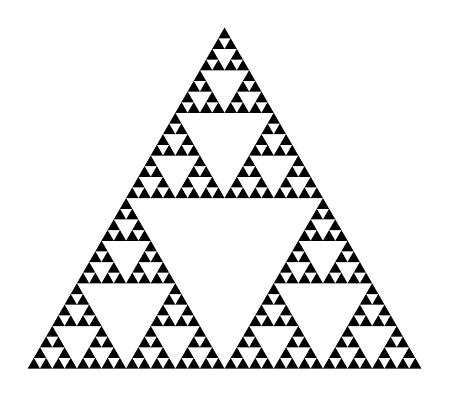
\begin{tikzpicture}[x=5cm,y=5cm]
      \fill (0.00000,0.00000) -- (0.03125,0.00000) -- (0.01562,0.02706) -- cycle;
\fill (0.03125,0.00000) -- (0.06250,0.00000) -- (0.04688,0.02706) -- cycle;
\fill (0.01562,0.02706) -- (0.04688,0.02706) -- (0.03125,0.05413) -- cycle;
\fill (0.06250,0.00000) -- (0.09375,0.00000) -- (0.07812,0.02706) -- cycle;
\fill (0.09375,0.00000) -- (0.12500,0.00000) -- (0.10938,0.02706) -- cycle;
\fill (0.07812,0.02706) -- (0.10938,0.02706) -- (0.09375,0.05413) -- cycle;
\fill (0.03125,0.05413) -- (0.06250,0.05413) -- (0.04688,0.08119) -- cycle;
\fill (0.06250,0.05413) -- (0.09375,0.05413) -- (0.07812,0.08119) -- cycle;
\fill (0.04688,0.08119) -- (0.07812,0.08119) -- (0.06250,0.10825) -- cycle;
\fill (0.12500,0.00000) -- (0.15625,0.00000) -- (0.14062,0.02706) -- cycle;
\fill (0.15625,0.00000) -- (0.18750,0.00000) -- (0.17188,0.02706) -- cycle;
\fill (0.14062,0.02706) -- (0.17188,0.02706) -- (0.15625,0.05413) -- cycle;
\fill (0.18750,0.00000) -- (0.21875,0.00000) -- (0.20312,0.02706) -- cycle;
\fill (0.21875,0.00000) -- (0.25000,0.00000) -- (0.23438,0.02706) -- cycle;
\fill (0.20312,0.02706) -- (0.23438,0.02706) -- (0.21875,0.05413) -- cycle;
\fill (0.15625,0.05413) -- (0.18750,0.05413) -- (0.17188,0.08119) -- cycle;
\fill (0.18750,0.05413) -- (0.21875,0.05413) -- (0.20312,0.08119) -- cycle;
\fill (0.17188,0.08119) -- (0.20312,0.08119) -- (0.18750,0.10825) -- cycle;
\fill (0.06250,0.10825) -- (0.09375,0.10825) -- (0.07812,0.13532) -- cycle;
\fill (0.09375,0.10825) -- (0.12500,0.10825) -- (0.10938,0.13532) -- cycle;
\fill (0.07812,0.13532) -- (0.10938,0.13532) -- (0.09375,0.16238) -- cycle;
\fill (0.12500,0.10825) -- (0.15625,0.10825) -- (0.14062,0.13532) -- cycle;
\fill (0.15625,0.10825) -- (0.18750,0.10825) -- (0.17188,0.13532) -- cycle;
\fill (0.14062,0.13532) -- (0.17188,0.13532) -- (0.15625,0.16238) -- cycle;
\fill (0.09375,0.16238) -- (0.12500,0.16238) -- (0.10938,0.18944) -- cycle;
\fill (0.12500,0.16238) -- (0.15625,0.16238) -- (0.14062,0.18944) -- cycle;
\fill (0.10938,0.18944) -- (0.14062,0.18944) -- (0.12500,0.21651) -- cycle;
\fill (0.25000,0.00000) -- (0.28125,0.00000) -- (0.26562,0.02706) -- cycle;
\fill (0.28125,0.00000) -- (0.31250,0.00000) -- (0.29688,0.02706) -- cycle;
\fill (0.26562,0.02706) -- (0.29688,0.02706) -- (0.28125,0.05413) -- cycle;
\fill (0.31250,0.00000) -- (0.34375,0.00000) -- (0.32812,0.02706) -- cycle;
\fill (0.34375,0.00000) -- (0.37500,0.00000) -- (0.35938,0.02706) -- cycle;
\fill (0.32812,0.02706) -- (0.35938,0.02706) -- (0.34375,0.05413) -- cycle;
\fill (0.28125,0.05413) -- (0.31250,0.05413) -- (0.29688,0.08119) -- cycle;
\fill (0.31250,0.05413) -- (0.34375,0.05413) -- (0.32812,0.08119) -- cycle;
\fill (0.29688,0.08119) -- (0.32812,0.08119) -- (0.31250,0.10825) -- cycle;
\fill (0.37500,0.00000) -- (0.40625,0.00000) -- (0.39062,0.02706) -- cycle;
\fill (0.40625,0.00000) -- (0.43750,0.00000) -- (0.42188,0.02706) -- cycle;
\fill (0.39062,0.02706) -- (0.42188,0.02706) -- (0.40625,0.05413) -- cycle;
\fill (0.43750,0.00000) -- (0.46875,0.00000) -- (0.45312,0.02706) -- cycle;
\fill (0.46875,0.00000) -- (0.50000,0.00000) -- (0.48438,0.02706) -- cycle;
\fill (0.45312,0.02706) -- (0.48438,0.02706) -- (0.46875,0.05413) -- cycle;
\fill (0.40625,0.05413) -- (0.43750,0.05413) -- (0.42188,0.08119) -- cycle;
\fill (0.43750,0.05413) -- (0.46875,0.05413) -- (0.45312,0.08119) -- cycle;
\fill (0.42188,0.08119) -- (0.45312,0.08119) -- (0.43750,0.10825) -- cycle;
\fill (0.31250,0.10825) -- (0.34375,0.10825) -- (0.32812,0.13532) -- cycle;
\fill (0.34375,0.10825) -- (0.37500,0.10825) -- (0.35938,0.13532) -- cycle;
\fill (0.32812,0.13532) -- (0.35938,0.13532) -- (0.34375,0.16238) -- cycle;
\fill (0.37500,0.10825) -- (0.40625,0.10825) -- (0.39062,0.13532) -- cycle;
\fill (0.40625,0.10825) -- (0.43750,0.10825) -- (0.42188,0.13532) -- cycle;
\fill (0.39062,0.13532) -- (0.42188,0.13532) -- (0.40625,0.16238) -- cycle;
\fill (0.34375,0.16238) -- (0.37500,0.16238) -- (0.35938,0.18944) -- cycle;
\fill (0.37500,0.16238) -- (0.40625,0.16238) -- (0.39062,0.18944) -- cycle;
\fill (0.35938,0.18944) -- (0.39062,0.18944) -- (0.37500,0.21651) -- cycle;
\fill (0.12500,0.21651) -- (0.15625,0.21651) -- (0.14062,0.24357) -- cycle;
\fill (0.15625,0.21651) -- (0.18750,0.21651) -- (0.17188,0.24357) -- cycle;
\fill (0.14062,0.24357) -- (0.17188,0.24357) -- (0.15625,0.27063) -- cycle;
\fill (0.18750,0.21651) -- (0.21875,0.21651) -- (0.20312,0.24357) -- cycle;
\fill (0.21875,0.21651) -- (0.25000,0.21651) -- (0.23438,0.24357) -- cycle;
\fill (0.20312,0.24357) -- (0.23438,0.24357) -- (0.21875,0.27063) -- cycle;
\fill (0.15625,0.27063) -- (0.18750,0.27063) -- (0.17188,0.29770) -- cycle;
\fill (0.18750,0.27063) -- (0.21875,0.27063) -- (0.20312,0.29770) -- cycle;
\fill (0.17188,0.29770) -- (0.20312,0.29770) -- (0.18750,0.32476) -- cycle;
\fill (0.25000,0.21651) -- (0.28125,0.21651) -- (0.26562,0.24357) -- cycle;
\fill (0.28125,0.21651) -- (0.31250,0.21651) -- (0.29688,0.24357) -- cycle;
\fill (0.26562,0.24357) -- (0.29688,0.24357) -- (0.28125,0.27063) -- cycle;
\fill (0.31250,0.21651) -- (0.34375,0.21651) -- (0.32812,0.24357) -- cycle;
\fill (0.34375,0.21651) -- (0.37500,0.21651) -- (0.35938,0.24357) -- cycle;
\fill (0.32812,0.24357) -- (0.35938,0.24357) -- (0.34375,0.27063) -- cycle;
\fill (0.28125,0.27063) -- (0.31250,0.27063) -- (0.29688,0.29770) -- cycle;
\fill (0.31250,0.27063) -- (0.34375,0.27063) -- (0.32812,0.29770) -- cycle;
\fill (0.29688,0.29770) -- (0.32812,0.29770) -- (0.31250,0.32476) -- cycle;
\fill (0.18750,0.32476) -- (0.21875,0.32476) -- (0.20312,0.35182) -- cycle;
\fill (0.21875,0.32476) -- (0.25000,0.32476) -- (0.23438,0.35182) -- cycle;
\fill (0.20312,0.35182) -- (0.23438,0.35182) -- (0.21875,0.37889) -- cycle;
\fill (0.25000,0.32476) -- (0.28125,0.32476) -- (0.26562,0.35182) -- cycle;
\fill (0.28125,0.32476) -- (0.31250,0.32476) -- (0.29688,0.35182) -- cycle;
\fill (0.26562,0.35182) -- (0.29688,0.35182) -- (0.28125,0.37889) -- cycle;
\fill (0.21875,0.37889) -- (0.25000,0.37889) -- (0.23438,0.40595) -- cycle;
\fill (0.25000,0.37889) -- (0.28125,0.37889) -- (0.26562,0.40595) -- cycle;
\fill (0.23438,0.40595) -- (0.26562,0.40595) -- (0.25000,0.43301) -- cycle;
\fill (0.50000,0.00000) -- (0.53125,0.00000) -- (0.51562,0.02706) -- cycle;
\fill (0.53125,0.00000) -- (0.56250,0.00000) -- (0.54688,0.02706) -- cycle;
\fill (0.51562,0.02706) -- (0.54688,0.02706) -- (0.53125,0.05413) -- cycle;
\fill (0.56250,0.00000) -- (0.59375,0.00000) -- (0.57812,0.02706) -- cycle;
\fill (0.59375,0.00000) -- (0.62500,0.00000) -- (0.60938,0.02706) -- cycle;
\fill (0.57812,0.02706) -- (0.60938,0.02706) -- (0.59375,0.05413) -- cycle;
\fill (0.53125,0.05413) -- (0.56250,0.05413) -- (0.54688,0.08119) -- cycle;
\fill (0.56250,0.05413) -- (0.59375,0.05413) -- (0.57812,0.08119) -- cycle;
\fill (0.54688,0.08119) -- (0.57812,0.08119) -- (0.56250,0.10825) -- cycle;
\fill (0.62500,0.00000) -- (0.65625,0.00000) -- (0.64062,0.02706) -- cycle;
\fill (0.65625,0.00000) -- (0.68750,0.00000) -- (0.67188,0.02706) -- cycle;
\fill (0.64062,0.02706) -- (0.67188,0.02706) -- (0.65625,0.05413) -- cycle;
\fill (0.68750,0.00000) -- (0.71875,0.00000) -- (0.70312,0.02706) -- cycle;
\fill (0.71875,0.00000) -- (0.75000,0.00000) -- (0.73438,0.02706) -- cycle;
\fill (0.70312,0.02706) -- (0.73438,0.02706) -- (0.71875,0.05413) -- cycle;
\fill (0.65625,0.05413) -- (0.68750,0.05413) -- (0.67188,0.08119) -- cycle;
\fill (0.68750,0.05413) -- (0.71875,0.05413) -- (0.70312,0.08119) -- cycle;
\fill (0.67188,0.08119) -- (0.70312,0.08119) -- (0.68750,0.10825) -- cycle;
\fill (0.56250,0.10825) -- (0.59375,0.10825) -- (0.57812,0.13532) -- cycle;
\fill (0.59375,0.10825) -- (0.62500,0.10825) -- (0.60938,0.13532) -- cycle;
\fill (0.57812,0.13532) -- (0.60938,0.13532) -- (0.59375,0.16238) -- cycle;
\fill (0.62500,0.10825) -- (0.65625,0.10825) -- (0.64062,0.13532) -- cycle;
\fill (0.65625,0.10825) -- (0.68750,0.10825) -- (0.67188,0.13532) -- cycle;
\fill (0.64062,0.13532) -- (0.67188,0.13532) -- (0.65625,0.16238) -- cycle;
\fill (0.59375,0.16238) -- (0.62500,0.16238) -- (0.60938,0.18944) -- cycle;
\fill (0.62500,0.16238) -- (0.65625,0.16238) -- (0.64062,0.18944) -- cycle;
\fill (0.60938,0.18944) -- (0.64062,0.18944) -- (0.62500,0.21651) -- cycle;
\fill (0.75000,0.00000) -- (0.78125,0.00000) -- (0.76562,0.02706) -- cycle;
\fill (0.78125,0.00000) -- (0.81250,0.00000) -- (0.79688,0.02706) -- cycle;
\fill (0.76562,0.02706) -- (0.79688,0.02706) -- (0.78125,0.05413) -- cycle;
\fill (0.81250,0.00000) -- (0.84375,0.00000) -- (0.82812,0.02706) -- cycle;
\fill (0.84375,0.00000) -- (0.87500,0.00000) -- (0.85938,0.02706) -- cycle;
\fill (0.82812,0.02706) -- (0.85938,0.02706) -- (0.84375,0.05413) -- cycle;
\fill (0.78125,0.05413) -- (0.81250,0.05413) -- (0.79688,0.08119) -- cycle;
\fill (0.81250,0.05413) -- (0.84375,0.05413) -- (0.82812,0.08119) -- cycle;
\fill (0.79688,0.08119) -- (0.82812,0.08119) -- (0.81250,0.10825) -- cycle;
\fill (0.87500,0.00000) -- (0.90625,0.00000) -- (0.89062,0.02706) -- cycle;
\fill (0.90625,0.00000) -- (0.93750,0.00000) -- (0.92188,0.02706) -- cycle;
\fill (0.89062,0.02706) -- (0.92188,0.02706) -- (0.90625,0.05413) -- cycle;
\fill (0.93750,0.00000) -- (0.96875,0.00000) -- (0.95312,0.02706) -- cycle;
\fill (0.96875,0.00000) -- (1.00000,0.00000) -- (0.98438,0.02706) -- cycle;
\fill (0.95312,0.02706) -- (0.98438,0.02706) -- (0.96875,0.05413) -- cycle;
\fill (0.90625,0.05413) -- (0.93750,0.05413) -- (0.92188,0.08119) -- cycle;
\fill (0.93750,0.05413) -- (0.96875,0.05413) -- (0.95312,0.08119) -- cycle;
\fill (0.92188,0.08119) -- (0.95312,0.08119) -- (0.93750,0.10825) -- cycle;
\fill (0.81250,0.10825) -- (0.84375,0.10825) -- (0.82812,0.13532) -- cycle;
\fill (0.84375,0.10825) -- (0.87500,0.10825) -- (0.85938,0.13532) -- cycle;
\fill (0.82812,0.13532) -- (0.85938,0.13532) -- (0.84375,0.16238) -- cycle;
\fill (0.87500,0.10825) -- (0.90625,0.10825) -- (0.89062,0.13532) -- cycle;
\fill (0.90625,0.10825) -- (0.93750,0.10825) -- (0.92188,0.13532) -- cycle;
\fill (0.89062,0.13532) -- (0.92188,0.13532) -- (0.90625,0.16238) -- cycle;
\fill (0.84375,0.16238) -- (0.87500,0.16238) -- (0.85938,0.18944) -- cycle;
\fill (0.87500,0.16238) -- (0.90625,0.16238) -- (0.89062,0.18944) -- cycle;
\fill (0.85938,0.18944) -- (0.89062,0.18944) -- (0.87500,0.21651) -- cycle;
\fill (0.62500,0.21651) -- (0.65625,0.21651) -- (0.64062,0.24357) -- cycle;
\fill (0.65625,0.21651) -- (0.68750,0.21651) -- (0.67188,0.24357) -- cycle;
\fill (0.64062,0.24357) -- (0.67188,0.24357) -- (0.65625,0.27063) -- cycle;
\fill (0.68750,0.21651) -- (0.71875,0.21651) -- (0.70312,0.24357) -- cycle;
\fill (0.71875,0.21651) -- (0.75000,0.21651) -- (0.73438,0.24357) -- cycle;
\fill (0.70312,0.24357) -- (0.73438,0.24357) -- (0.71875,0.27063) -- cycle;
\fill (0.65625,0.27063) -- (0.68750,0.27063) -- (0.67188,0.29770) -- cycle;
\fill (0.68750,0.27063) -- (0.71875,0.27063) -- (0.70312,0.29770) -- cycle;
\fill (0.67188,0.29770) -- (0.70312,0.29770) -- (0.68750,0.32476) -- cycle;
\fill (0.75000,0.21651) -- (0.78125,0.21651) -- (0.76562,0.24357) -- cycle;
\fill (0.78125,0.21651) -- (0.81250,0.21651) -- (0.79688,0.24357) -- cycle;
\fill (0.76562,0.24357) -- (0.79688,0.24357) -- (0.78125,0.27063) -- cycle;
\fill (0.81250,0.21651) -- (0.84375,0.21651) -- (0.82812,0.24357) -- cycle;
\fill (0.84375,0.21651) -- (0.87500,0.21651) -- (0.85938,0.24357) -- cycle;
\fill (0.82812,0.24357) -- (0.85938,0.24357) -- (0.84375,0.27063) -- cycle;
\fill (0.78125,0.27063) -- (0.81250,0.27063) -- (0.79688,0.29770) -- cycle;
\fill (0.81250,0.27063) -- (0.84375,0.27063) -- (0.82812,0.29770) -- cycle;
\fill (0.79688,0.29770) -- (0.82812,0.29770) -- (0.81250,0.32476) -- cycle;
\fill (0.68750,0.32476) -- (0.71875,0.32476) -- (0.70312,0.35182) -- cycle;
\fill (0.71875,0.32476) -- (0.75000,0.32476) -- (0.73438,0.35182) -- cycle;
\fill (0.70312,0.35182) -- (0.73438,0.35182) -- (0.71875,0.37889) -- cycle;
\fill (0.75000,0.32476) -- (0.78125,0.32476) -- (0.76562,0.35182) -- cycle;
\fill (0.78125,0.32476) -- (0.81250,0.32476) -- (0.79688,0.35182) -- cycle;
\fill (0.76562,0.35182) -- (0.79688,0.35182) -- (0.78125,0.37889) -- cycle;
\fill (0.71875,0.37889) -- (0.75000,0.37889) -- (0.73438,0.40595) -- cycle;
\fill (0.75000,0.37889) -- (0.78125,0.37889) -- (0.76562,0.40595) -- cycle;
\fill (0.73438,0.40595) -- (0.76562,0.40595) -- (0.75000,0.43301) -- cycle;
\fill (0.25000,0.43301) -- (0.28125,0.43301) -- (0.26562,0.46008) -- cycle;
\fill (0.28125,0.43301) -- (0.31250,0.43301) -- (0.29688,0.46008) -- cycle;
\fill (0.26562,0.46008) -- (0.29688,0.46008) -- (0.28125,0.48714) -- cycle;
\fill (0.31250,0.43301) -- (0.34375,0.43301) -- (0.32812,0.46008) -- cycle;
\fill (0.34375,0.43301) -- (0.37500,0.43301) -- (0.35938,0.46008) -- cycle;
\fill (0.32812,0.46008) -- (0.35938,0.46008) -- (0.34375,0.48714) -- cycle;
\fill (0.28125,0.48714) -- (0.31250,0.48714) -- (0.29688,0.51420) -- cycle;
\fill (0.31250,0.48714) -- (0.34375,0.48714) -- (0.32812,0.51420) -- cycle;
\fill (0.29688,0.51420) -- (0.32812,0.51420) -- (0.31250,0.54127) -- cycle;
\fill (0.37500,0.43301) -- (0.40625,0.43301) -- (0.39062,0.46008) -- cycle;
\fill (0.40625,0.43301) -- (0.43750,0.43301) -- (0.42188,0.46008) -- cycle;
\fill (0.39062,0.46008) -- (0.42188,0.46008) -- (0.40625,0.48714) -- cycle;
\fill (0.43750,0.43301) -- (0.46875,0.43301) -- (0.45312,0.46008) -- cycle;
\fill (0.46875,0.43301) -- (0.50000,0.43301) -- (0.48438,0.46008) -- cycle;
\fill (0.45312,0.46008) -- (0.48438,0.46008) -- (0.46875,0.48714) -- cycle;
\fill (0.40625,0.48714) -- (0.43750,0.48714) -- (0.42188,0.51420) -- cycle;
\fill (0.43750,0.48714) -- (0.46875,0.48714) -- (0.45312,0.51420) -- cycle;
\fill (0.42188,0.51420) -- (0.45312,0.51420) -- (0.43750,0.54127) -- cycle;
\fill (0.31250,0.54127) -- (0.34375,0.54127) -- (0.32812,0.56833) -- cycle;
\fill (0.34375,0.54127) -- (0.37500,0.54127) -- (0.35938,0.56833) -- cycle;
\fill (0.32812,0.56833) -- (0.35938,0.56833) -- (0.34375,0.59539) -- cycle;
\fill (0.37500,0.54127) -- (0.40625,0.54127) -- (0.39062,0.56833) -- cycle;
\fill (0.40625,0.54127) -- (0.43750,0.54127) -- (0.42188,0.56833) -- cycle;
\fill (0.39062,0.56833) -- (0.42188,0.56833) -- (0.40625,0.59539) -- cycle;
\fill (0.34375,0.59539) -- (0.37500,0.59539) -- (0.35938,0.62246) -- cycle;
\fill (0.37500,0.59539) -- (0.40625,0.59539) -- (0.39062,0.62246) -- cycle;
\fill (0.35938,0.62246) -- (0.39062,0.62246) -- (0.37500,0.64952) -- cycle;
\fill (0.50000,0.43301) -- (0.53125,0.43301) -- (0.51562,0.46008) -- cycle;
\fill (0.53125,0.43301) -- (0.56250,0.43301) -- (0.54688,0.46008) -- cycle;
\fill (0.51562,0.46008) -- (0.54688,0.46008) -- (0.53125,0.48714) -- cycle;
\fill (0.56250,0.43301) -- (0.59375,0.43301) -- (0.57812,0.46008) -- cycle;
\fill (0.59375,0.43301) -- (0.62500,0.43301) -- (0.60938,0.46008) -- cycle;
\fill (0.57812,0.46008) -- (0.60938,0.46008) -- (0.59375,0.48714) -- cycle;
\fill (0.53125,0.48714) -- (0.56250,0.48714) -- (0.54688,0.51420) -- cycle;
\fill (0.56250,0.48714) -- (0.59375,0.48714) -- (0.57812,0.51420) -- cycle;
\fill (0.54688,0.51420) -- (0.57812,0.51420) -- (0.56250,0.54127) -- cycle;
\fill (0.62500,0.43301) -- (0.65625,0.43301) -- (0.64062,0.46008) -- cycle;
\fill (0.65625,0.43301) -- (0.68750,0.43301) -- (0.67188,0.46008) -- cycle;
\fill (0.64062,0.46008) -- (0.67188,0.46008) -- (0.65625,0.48714) -- cycle;
\fill (0.68750,0.43301) -- (0.71875,0.43301) -- (0.70312,0.46008) -- cycle;
\fill (0.71875,0.43301) -- (0.75000,0.43301) -- (0.73438,0.46008) -- cycle;
\fill (0.70312,0.46008) -- (0.73438,0.46008) -- (0.71875,0.48714) -- cycle;
\fill (0.65625,0.48714) -- (0.68750,0.48714) -- (0.67188,0.51420) -- cycle;
\fill (0.68750,0.48714) -- (0.71875,0.48714) -- (0.70312,0.51420) -- cycle;
\fill (0.67188,0.51420) -- (0.70312,0.51420) -- (0.68750,0.54127) -- cycle;
\fill (0.56250,0.54127) -- (0.59375,0.54127) -- (0.57812,0.56833) -- cycle;
\fill (0.59375,0.54127) -- (0.62500,0.54127) -- (0.60938,0.56833) -- cycle;
\fill (0.57812,0.56833) -- (0.60938,0.56833) -- (0.59375,0.59539) -- cycle;
\fill (0.62500,0.54127) -- (0.65625,0.54127) -- (0.64062,0.56833) -- cycle;
\fill (0.65625,0.54127) -- (0.68750,0.54127) -- (0.67188,0.56833) -- cycle;
\fill (0.64062,0.56833) -- (0.67188,0.56833) -- (0.65625,0.59539) -- cycle;
\fill (0.59375,0.59539) -- (0.62500,0.59539) -- (0.60938,0.62246) -- cycle;
\fill (0.62500,0.59539) -- (0.65625,0.59539) -- (0.64062,0.62246) -- cycle;
\fill (0.60938,0.62246) -- (0.64062,0.62246) -- (0.62500,0.64952) -- cycle;
\fill (0.37500,0.64952) -- (0.40625,0.64952) -- (0.39062,0.67658) -- cycle;
\fill (0.40625,0.64952) -- (0.43750,0.64952) -- (0.42188,0.67658) -- cycle;
\fill (0.39062,0.67658) -- (0.42188,0.67658) -- (0.40625,0.70365) -- cycle;
\fill (0.43750,0.64952) -- (0.46875,0.64952) -- (0.45312,0.67658) -- cycle;
\fill (0.46875,0.64952) -- (0.50000,0.64952) -- (0.48438,0.67658) -- cycle;
\fill (0.45312,0.67658) -- (0.48438,0.67658) -- (0.46875,0.70365) -- cycle;
\fill (0.40625,0.70365) -- (0.43750,0.70365) -- (0.42188,0.73071) -- cycle;
\fill (0.43750,0.70365) -- (0.46875,0.70365) -- (0.45312,0.73071) -- cycle;
\fill (0.42188,0.73071) -- (0.45312,0.73071) -- (0.43750,0.75777) -- cycle;
\fill (0.50000,0.64952) -- (0.53125,0.64952) -- (0.51562,0.67658) -- cycle;
\fill (0.53125,0.64952) -- (0.56250,0.64952) -- (0.54688,0.67658) -- cycle;
\fill (0.51562,0.67658) -- (0.54688,0.67658) -- (0.53125,0.70365) -- cycle;
\fill (0.56250,0.64952) -- (0.59375,0.64952) -- (0.57812,0.67658) -- cycle;
\fill (0.59375,0.64952) -- (0.62500,0.64952) -- (0.60938,0.67658) -- cycle;
\fill (0.57812,0.67658) -- (0.60938,0.67658) -- (0.59375,0.70365) -- cycle;
\fill (0.53125,0.70365) -- (0.56250,0.70365) -- (0.54688,0.73071) -- cycle;
\fill (0.56250,0.70365) -- (0.59375,0.70365) -- (0.57812,0.73071) -- cycle;
\fill (0.54688,0.73071) -- (0.57812,0.73071) -- (0.56250,0.75777) -- cycle;
\fill (0.43750,0.75777) -- (0.46875,0.75777) -- (0.45312,0.78484) -- cycle;
\fill (0.46875,0.75777) -- (0.50000,0.75777) -- (0.48438,0.78484) -- cycle;
\fill (0.45312,0.78484) -- (0.48438,0.78484) -- (0.46875,0.81190) -- cycle;
\fill (0.50000,0.75777) -- (0.53125,0.75777) -- (0.51562,0.78484) -- cycle;
\fill (0.53125,0.75777) -- (0.56250,0.75777) -- (0.54688,0.78484) -- cycle;
\fill (0.51562,0.78484) -- (0.54688,0.78484) -- (0.53125,0.81190) -- cycle;
\fill (0.46875,0.81190) -- (0.50000,0.81190) -- (0.48438,0.83896) -- cycle;
\fill (0.50000,0.81190) -- (0.53125,0.81190) -- (0.51562,0.83896) -- cycle;
\fill (0.48438,0.83896) -- (0.51562,0.83896) -- (0.50000,0.86603) -- cycle;

    \end{tikzpicture}
    \caption{Сјерпињски троугао}
  \end{subfigure}

  \vspace{1em}

  \begin{subfigure}[b]{0.45\textwidth}
    \centering
    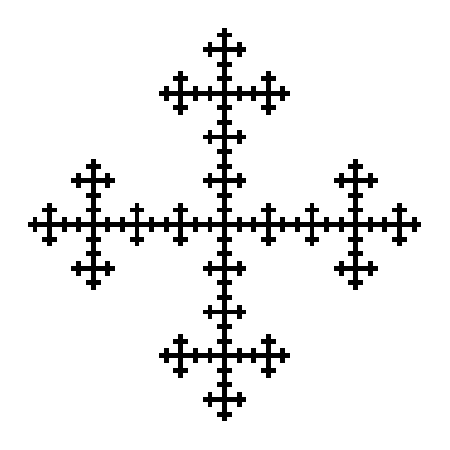
\begin{tikzpicture}[x=5cm,y=5cm]
      \fill (0.00000,0.49383) rectangle (0.01235,0.50617);
\fill (0.01235,0.50617) rectangle (0.02469,0.51852);
\fill (0.02469,0.49383) rectangle (0.03704,0.50617);
\fill (0.01235,0.48148) rectangle (0.02469,0.49383);
\fill (0.01235,0.49383) rectangle (0.02469,0.50617);
\fill (0.03704,0.53086) rectangle (0.04938,0.54321);
\fill (0.04938,0.54321) rectangle (0.06173,0.55556);
\fill (0.06173,0.53086) rectangle (0.07407,0.54321);
\fill (0.04938,0.51852) rectangle (0.06173,0.53086);
\fill (0.04938,0.53086) rectangle (0.06173,0.54321);
\fill (0.07407,0.49383) rectangle (0.08642,0.50617);
\fill (0.08642,0.50617) rectangle (0.09877,0.51852);
\fill (0.09877,0.49383) rectangle (0.11111,0.50617);
\fill (0.08642,0.48148) rectangle (0.09877,0.49383);
\fill (0.08642,0.49383) rectangle (0.09877,0.50617);
\fill (0.03704,0.45679) rectangle (0.04938,0.46914);
\fill (0.04938,0.46914) rectangle (0.06173,0.48148);
\fill (0.06173,0.45679) rectangle (0.07407,0.46914);
\fill (0.04938,0.44444) rectangle (0.06173,0.45679);
\fill (0.04938,0.45679) rectangle (0.06173,0.46914);
\fill (0.03704,0.49383) rectangle (0.04938,0.50617);
\fill (0.04938,0.50617) rectangle (0.06173,0.51852);
\fill (0.06173,0.49383) rectangle (0.07407,0.50617);
\fill (0.04938,0.48148) rectangle (0.06173,0.49383);
\fill (0.04938,0.49383) rectangle (0.06173,0.50617);
\fill (0.11111,0.60494) rectangle (0.12346,0.61728);
\fill (0.12346,0.61728) rectangle (0.13580,0.62963);
\fill (0.13580,0.60494) rectangle (0.14815,0.61728);
\fill (0.12346,0.59259) rectangle (0.13580,0.60494);
\fill (0.12346,0.60494) rectangle (0.13580,0.61728);
\fill (0.14815,0.64198) rectangle (0.16049,0.65432);
\fill (0.16049,0.65432) rectangle (0.17284,0.66667);
\fill (0.17284,0.64198) rectangle (0.18519,0.65432);
\fill (0.16049,0.62963) rectangle (0.17284,0.64198);
\fill (0.16049,0.64198) rectangle (0.17284,0.65432);
\fill (0.18519,0.60494) rectangle (0.19753,0.61728);
\fill (0.19753,0.61728) rectangle (0.20988,0.62963);
\fill (0.20988,0.60494) rectangle (0.22222,0.61728);
\fill (0.19753,0.59259) rectangle (0.20988,0.60494);
\fill (0.19753,0.60494) rectangle (0.20988,0.61728);
\fill (0.14815,0.56790) rectangle (0.16049,0.58025);
\fill (0.16049,0.58025) rectangle (0.17284,0.59259);
\fill (0.17284,0.56790) rectangle (0.18519,0.58025);
\fill (0.16049,0.55556) rectangle (0.17284,0.56790);
\fill (0.16049,0.56790) rectangle (0.17284,0.58025);
\fill (0.14815,0.60494) rectangle (0.16049,0.61728);
\fill (0.16049,0.61728) rectangle (0.17284,0.62963);
\fill (0.17284,0.60494) rectangle (0.18519,0.61728);
\fill (0.16049,0.59259) rectangle (0.17284,0.60494);
\fill (0.16049,0.60494) rectangle (0.17284,0.61728);
\fill (0.22222,0.49383) rectangle (0.23457,0.50617);
\fill (0.23457,0.50617) rectangle (0.24691,0.51852);
\fill (0.24691,0.49383) rectangle (0.25926,0.50617);
\fill (0.23457,0.48148) rectangle (0.24691,0.49383);
\fill (0.23457,0.49383) rectangle (0.24691,0.50617);
\fill (0.25926,0.53086) rectangle (0.27160,0.54321);
\fill (0.27160,0.54321) rectangle (0.28395,0.55556);
\fill (0.28395,0.53086) rectangle (0.29630,0.54321);
\fill (0.27160,0.51852) rectangle (0.28395,0.53086);
\fill (0.27160,0.53086) rectangle (0.28395,0.54321);
\fill (0.29630,0.49383) rectangle (0.30864,0.50617);
\fill (0.30864,0.50617) rectangle (0.32099,0.51852);
\fill (0.32099,0.49383) rectangle (0.33333,0.50617);
\fill (0.30864,0.48148) rectangle (0.32099,0.49383);
\fill (0.30864,0.49383) rectangle (0.32099,0.50617);
\fill (0.25926,0.45679) rectangle (0.27160,0.46914);
\fill (0.27160,0.46914) rectangle (0.28395,0.48148);
\fill (0.28395,0.45679) rectangle (0.29630,0.46914);
\fill (0.27160,0.44444) rectangle (0.28395,0.45679);
\fill (0.27160,0.45679) rectangle (0.28395,0.46914);
\fill (0.25926,0.49383) rectangle (0.27160,0.50617);
\fill (0.27160,0.50617) rectangle (0.28395,0.51852);
\fill (0.28395,0.49383) rectangle (0.29630,0.50617);
\fill (0.27160,0.48148) rectangle (0.28395,0.49383);
\fill (0.27160,0.49383) rectangle (0.28395,0.50617);
\fill (0.11111,0.38272) rectangle (0.12346,0.39506);
\fill (0.12346,0.39506) rectangle (0.13580,0.40741);
\fill (0.13580,0.38272) rectangle (0.14815,0.39506);
\fill (0.12346,0.37037) rectangle (0.13580,0.38272);
\fill (0.12346,0.38272) rectangle (0.13580,0.39506);
\fill (0.14815,0.41975) rectangle (0.16049,0.43210);
\fill (0.16049,0.43210) rectangle (0.17284,0.44444);
\fill (0.17284,0.41975) rectangle (0.18519,0.43210);
\fill (0.16049,0.40741) rectangle (0.17284,0.41975);
\fill (0.16049,0.41975) rectangle (0.17284,0.43210);
\fill (0.18519,0.38272) rectangle (0.19753,0.39506);
\fill (0.19753,0.39506) rectangle (0.20988,0.40741);
\fill (0.20988,0.38272) rectangle (0.22222,0.39506);
\fill (0.19753,0.37037) rectangle (0.20988,0.38272);
\fill (0.19753,0.38272) rectangle (0.20988,0.39506);
\fill (0.14815,0.34568) rectangle (0.16049,0.35802);
\fill (0.16049,0.35802) rectangle (0.17284,0.37037);
\fill (0.17284,0.34568) rectangle (0.18519,0.35802);
\fill (0.16049,0.33333) rectangle (0.17284,0.34568);
\fill (0.16049,0.34568) rectangle (0.17284,0.35802);
\fill (0.14815,0.38272) rectangle (0.16049,0.39506);
\fill (0.16049,0.39506) rectangle (0.17284,0.40741);
\fill (0.17284,0.38272) rectangle (0.18519,0.39506);
\fill (0.16049,0.37037) rectangle (0.17284,0.38272);
\fill (0.16049,0.38272) rectangle (0.17284,0.39506);
\fill (0.11111,0.49383) rectangle (0.12346,0.50617);
\fill (0.12346,0.50617) rectangle (0.13580,0.51852);
\fill (0.13580,0.49383) rectangle (0.14815,0.50617);
\fill (0.12346,0.48148) rectangle (0.13580,0.49383);
\fill (0.12346,0.49383) rectangle (0.13580,0.50617);
\fill (0.14815,0.53086) rectangle (0.16049,0.54321);
\fill (0.16049,0.54321) rectangle (0.17284,0.55556);
\fill (0.17284,0.53086) rectangle (0.18519,0.54321);
\fill (0.16049,0.51852) rectangle (0.17284,0.53086);
\fill (0.16049,0.53086) rectangle (0.17284,0.54321);
\fill (0.18519,0.49383) rectangle (0.19753,0.50617);
\fill (0.19753,0.50617) rectangle (0.20988,0.51852);
\fill (0.20988,0.49383) rectangle (0.22222,0.50617);
\fill (0.19753,0.48148) rectangle (0.20988,0.49383);
\fill (0.19753,0.49383) rectangle (0.20988,0.50617);
\fill (0.14815,0.45679) rectangle (0.16049,0.46914);
\fill (0.16049,0.46914) rectangle (0.17284,0.48148);
\fill (0.17284,0.45679) rectangle (0.18519,0.46914);
\fill (0.16049,0.44444) rectangle (0.17284,0.45679);
\fill (0.16049,0.45679) rectangle (0.17284,0.46914);
\fill (0.14815,0.49383) rectangle (0.16049,0.50617);
\fill (0.16049,0.50617) rectangle (0.17284,0.51852);
\fill (0.17284,0.49383) rectangle (0.18519,0.50617);
\fill (0.16049,0.48148) rectangle (0.17284,0.49383);
\fill (0.16049,0.49383) rectangle (0.17284,0.50617);
\fill (0.33333,0.82716) rectangle (0.34568,0.83951);
\fill (0.34568,0.83951) rectangle (0.35802,0.85185);
\fill (0.35802,0.82716) rectangle (0.37037,0.83951);
\fill (0.34568,0.81481) rectangle (0.35802,0.82716);
\fill (0.34568,0.82716) rectangle (0.35802,0.83951);
\fill (0.37037,0.86420) rectangle (0.38272,0.87654);
\fill (0.38272,0.87654) rectangle (0.39506,0.88889);
\fill (0.39506,0.86420) rectangle (0.40741,0.87654);
\fill (0.38272,0.85185) rectangle (0.39506,0.86420);
\fill (0.38272,0.86420) rectangle (0.39506,0.87654);
\fill (0.40741,0.82716) rectangle (0.41975,0.83951);
\fill (0.41975,0.83951) rectangle (0.43210,0.85185);
\fill (0.43210,0.82716) rectangle (0.44444,0.83951);
\fill (0.41975,0.81481) rectangle (0.43210,0.82716);
\fill (0.41975,0.82716) rectangle (0.43210,0.83951);
\fill (0.37037,0.79012) rectangle (0.38272,0.80247);
\fill (0.38272,0.80247) rectangle (0.39506,0.81481);
\fill (0.39506,0.79012) rectangle (0.40741,0.80247);
\fill (0.38272,0.77778) rectangle (0.39506,0.79012);
\fill (0.38272,0.79012) rectangle (0.39506,0.80247);
\fill (0.37037,0.82716) rectangle (0.38272,0.83951);
\fill (0.38272,0.83951) rectangle (0.39506,0.85185);
\fill (0.39506,0.82716) rectangle (0.40741,0.83951);
\fill (0.38272,0.81481) rectangle (0.39506,0.82716);
\fill (0.38272,0.82716) rectangle (0.39506,0.83951);
\fill (0.44444,0.93827) rectangle (0.45679,0.95062);
\fill (0.45679,0.95062) rectangle (0.46914,0.96296);
\fill (0.46914,0.93827) rectangle (0.48148,0.95062);
\fill (0.45679,0.92593) rectangle (0.46914,0.93827);
\fill (0.45679,0.93827) rectangle (0.46914,0.95062);
\fill (0.48148,0.97531) rectangle (0.49383,0.98765);
\fill (0.49383,0.98765) rectangle (0.50617,1.00000);
\fill (0.50617,0.97531) rectangle (0.51852,0.98765);
\fill (0.49383,0.96296) rectangle (0.50617,0.97531);
\fill (0.49383,0.97531) rectangle (0.50617,0.98765);
\fill (0.51852,0.93827) rectangle (0.53086,0.95062);
\fill (0.53086,0.95062) rectangle (0.54321,0.96296);
\fill (0.54321,0.93827) rectangle (0.55556,0.95062);
\fill (0.53086,0.92593) rectangle (0.54321,0.93827);
\fill (0.53086,0.93827) rectangle (0.54321,0.95062);
\fill (0.48148,0.90123) rectangle (0.49383,0.91358);
\fill (0.49383,0.91358) rectangle (0.50617,0.92593);
\fill (0.50617,0.90123) rectangle (0.51852,0.91358);
\fill (0.49383,0.88889) rectangle (0.50617,0.90123);
\fill (0.49383,0.90123) rectangle (0.50617,0.91358);
\fill (0.48148,0.93827) rectangle (0.49383,0.95062);
\fill (0.49383,0.95062) rectangle (0.50617,0.96296);
\fill (0.50617,0.93827) rectangle (0.51852,0.95062);
\fill (0.49383,0.92593) rectangle (0.50617,0.93827);
\fill (0.49383,0.93827) rectangle (0.50617,0.95062);
\fill (0.55556,0.82716) rectangle (0.56790,0.83951);
\fill (0.56790,0.83951) rectangle (0.58025,0.85185);
\fill (0.58025,0.82716) rectangle (0.59259,0.83951);
\fill (0.56790,0.81481) rectangle (0.58025,0.82716);
\fill (0.56790,0.82716) rectangle (0.58025,0.83951);
\fill (0.59259,0.86420) rectangle (0.60494,0.87654);
\fill (0.60494,0.87654) rectangle (0.61728,0.88889);
\fill (0.61728,0.86420) rectangle (0.62963,0.87654);
\fill (0.60494,0.85185) rectangle (0.61728,0.86420);
\fill (0.60494,0.86420) rectangle (0.61728,0.87654);
\fill (0.62963,0.82716) rectangle (0.64198,0.83951);
\fill (0.64198,0.83951) rectangle (0.65432,0.85185);
\fill (0.65432,0.82716) rectangle (0.66667,0.83951);
\fill (0.64198,0.81481) rectangle (0.65432,0.82716);
\fill (0.64198,0.82716) rectangle (0.65432,0.83951);
\fill (0.59259,0.79012) rectangle (0.60494,0.80247);
\fill (0.60494,0.80247) rectangle (0.61728,0.81481);
\fill (0.61728,0.79012) rectangle (0.62963,0.80247);
\fill (0.60494,0.77778) rectangle (0.61728,0.79012);
\fill (0.60494,0.79012) rectangle (0.61728,0.80247);
\fill (0.59259,0.82716) rectangle (0.60494,0.83951);
\fill (0.60494,0.83951) rectangle (0.61728,0.85185);
\fill (0.61728,0.82716) rectangle (0.62963,0.83951);
\fill (0.60494,0.81481) rectangle (0.61728,0.82716);
\fill (0.60494,0.82716) rectangle (0.61728,0.83951);
\fill (0.44444,0.71605) rectangle (0.45679,0.72840);
\fill (0.45679,0.72840) rectangle (0.46914,0.74074);
\fill (0.46914,0.71605) rectangle (0.48148,0.72840);
\fill (0.45679,0.70370) rectangle (0.46914,0.71605);
\fill (0.45679,0.71605) rectangle (0.46914,0.72840);
\fill (0.48148,0.75309) rectangle (0.49383,0.76543);
\fill (0.49383,0.76543) rectangle (0.50617,0.77778);
\fill (0.50617,0.75309) rectangle (0.51852,0.76543);
\fill (0.49383,0.74074) rectangle (0.50617,0.75309);
\fill (0.49383,0.75309) rectangle (0.50617,0.76543);
\fill (0.51852,0.71605) rectangle (0.53086,0.72840);
\fill (0.53086,0.72840) rectangle (0.54321,0.74074);
\fill (0.54321,0.71605) rectangle (0.55556,0.72840);
\fill (0.53086,0.70370) rectangle (0.54321,0.71605);
\fill (0.53086,0.71605) rectangle (0.54321,0.72840);
\fill (0.48148,0.67901) rectangle (0.49383,0.69136);
\fill (0.49383,0.69136) rectangle (0.50617,0.70370);
\fill (0.50617,0.67901) rectangle (0.51852,0.69136);
\fill (0.49383,0.66667) rectangle (0.50617,0.67901);
\fill (0.49383,0.67901) rectangle (0.50617,0.69136);
\fill (0.48148,0.71605) rectangle (0.49383,0.72840);
\fill (0.49383,0.72840) rectangle (0.50617,0.74074);
\fill (0.50617,0.71605) rectangle (0.51852,0.72840);
\fill (0.49383,0.70370) rectangle (0.50617,0.71605);
\fill (0.49383,0.71605) rectangle (0.50617,0.72840);
\fill (0.44444,0.82716) rectangle (0.45679,0.83951);
\fill (0.45679,0.83951) rectangle (0.46914,0.85185);
\fill (0.46914,0.82716) rectangle (0.48148,0.83951);
\fill (0.45679,0.81481) rectangle (0.46914,0.82716);
\fill (0.45679,0.82716) rectangle (0.46914,0.83951);
\fill (0.48148,0.86420) rectangle (0.49383,0.87654);
\fill (0.49383,0.87654) rectangle (0.50617,0.88889);
\fill (0.50617,0.86420) rectangle (0.51852,0.87654);
\fill (0.49383,0.85185) rectangle (0.50617,0.86420);
\fill (0.49383,0.86420) rectangle (0.50617,0.87654);
\fill (0.51852,0.82716) rectangle (0.53086,0.83951);
\fill (0.53086,0.83951) rectangle (0.54321,0.85185);
\fill (0.54321,0.82716) rectangle (0.55556,0.83951);
\fill (0.53086,0.81481) rectangle (0.54321,0.82716);
\fill (0.53086,0.82716) rectangle (0.54321,0.83951);
\fill (0.48148,0.79012) rectangle (0.49383,0.80247);
\fill (0.49383,0.80247) rectangle (0.50617,0.81481);
\fill (0.50617,0.79012) rectangle (0.51852,0.80247);
\fill (0.49383,0.77778) rectangle (0.50617,0.79012);
\fill (0.49383,0.79012) rectangle (0.50617,0.80247);
\fill (0.48148,0.82716) rectangle (0.49383,0.83951);
\fill (0.49383,0.83951) rectangle (0.50617,0.85185);
\fill (0.50617,0.82716) rectangle (0.51852,0.83951);
\fill (0.49383,0.81481) rectangle (0.50617,0.82716);
\fill (0.49383,0.82716) rectangle (0.50617,0.83951);
\fill (0.66667,0.49383) rectangle (0.67901,0.50617);
\fill (0.67901,0.50617) rectangle (0.69136,0.51852);
\fill (0.69136,0.49383) rectangle (0.70370,0.50617);
\fill (0.67901,0.48148) rectangle (0.69136,0.49383);
\fill (0.67901,0.49383) rectangle (0.69136,0.50617);
\fill (0.70370,0.53086) rectangle (0.71605,0.54321);
\fill (0.71605,0.54321) rectangle (0.72840,0.55556);
\fill (0.72840,0.53086) rectangle (0.74074,0.54321);
\fill (0.71605,0.51852) rectangle (0.72840,0.53086);
\fill (0.71605,0.53086) rectangle (0.72840,0.54321);
\fill (0.74074,0.49383) rectangle (0.75309,0.50617);
\fill (0.75309,0.50617) rectangle (0.76543,0.51852);
\fill (0.76543,0.49383) rectangle (0.77778,0.50617);
\fill (0.75309,0.48148) rectangle (0.76543,0.49383);
\fill (0.75309,0.49383) rectangle (0.76543,0.50617);
\fill (0.70370,0.45679) rectangle (0.71605,0.46914);
\fill (0.71605,0.46914) rectangle (0.72840,0.48148);
\fill (0.72840,0.45679) rectangle (0.74074,0.46914);
\fill (0.71605,0.44444) rectangle (0.72840,0.45679);
\fill (0.71605,0.45679) rectangle (0.72840,0.46914);
\fill (0.70370,0.49383) rectangle (0.71605,0.50617);
\fill (0.71605,0.50617) rectangle (0.72840,0.51852);
\fill (0.72840,0.49383) rectangle (0.74074,0.50617);
\fill (0.71605,0.48148) rectangle (0.72840,0.49383);
\fill (0.71605,0.49383) rectangle (0.72840,0.50617);
\fill (0.77778,0.60494) rectangle (0.79012,0.61728);
\fill (0.79012,0.61728) rectangle (0.80247,0.62963);
\fill (0.80247,0.60494) rectangle (0.81481,0.61728);
\fill (0.79012,0.59259) rectangle (0.80247,0.60494);
\fill (0.79012,0.60494) rectangle (0.80247,0.61728);
\fill (0.81481,0.64198) rectangle (0.82716,0.65432);
\fill (0.82716,0.65432) rectangle (0.83951,0.66667);
\fill (0.83951,0.64198) rectangle (0.85185,0.65432);
\fill (0.82716,0.62963) rectangle (0.83951,0.64198);
\fill (0.82716,0.64198) rectangle (0.83951,0.65432);
\fill (0.85185,0.60494) rectangle (0.86420,0.61728);
\fill (0.86420,0.61728) rectangle (0.87654,0.62963);
\fill (0.87654,0.60494) rectangle (0.88889,0.61728);
\fill (0.86420,0.59259) rectangle (0.87654,0.60494);
\fill (0.86420,0.60494) rectangle (0.87654,0.61728);
\fill (0.81481,0.56790) rectangle (0.82716,0.58025);
\fill (0.82716,0.58025) rectangle (0.83951,0.59259);
\fill (0.83951,0.56790) rectangle (0.85185,0.58025);
\fill (0.82716,0.55556) rectangle (0.83951,0.56790);
\fill (0.82716,0.56790) rectangle (0.83951,0.58025);
\fill (0.81481,0.60494) rectangle (0.82716,0.61728);
\fill (0.82716,0.61728) rectangle (0.83951,0.62963);
\fill (0.83951,0.60494) rectangle (0.85185,0.61728);
\fill (0.82716,0.59259) rectangle (0.83951,0.60494);
\fill (0.82716,0.60494) rectangle (0.83951,0.61728);
\fill (0.88889,0.49383) rectangle (0.90123,0.50617);
\fill (0.90123,0.50617) rectangle (0.91358,0.51852);
\fill (0.91358,0.49383) rectangle (0.92593,0.50617);
\fill (0.90123,0.48148) rectangle (0.91358,0.49383);
\fill (0.90123,0.49383) rectangle (0.91358,0.50617);
\fill (0.92593,0.53086) rectangle (0.93827,0.54321);
\fill (0.93827,0.54321) rectangle (0.95062,0.55556);
\fill (0.95062,0.53086) rectangle (0.96296,0.54321);
\fill (0.93827,0.51852) rectangle (0.95062,0.53086);
\fill (0.93827,0.53086) rectangle (0.95062,0.54321);
\fill (0.96296,0.49383) rectangle (0.97531,0.50617);
\fill (0.97531,0.50617) rectangle (0.98765,0.51852);
\fill (0.98765,0.49383) rectangle (1.00000,0.50617);
\fill (0.97531,0.48148) rectangle (0.98765,0.49383);
\fill (0.97531,0.49383) rectangle (0.98765,0.50617);
\fill (0.92593,0.45679) rectangle (0.93827,0.46914);
\fill (0.93827,0.46914) rectangle (0.95062,0.48148);
\fill (0.95062,0.45679) rectangle (0.96296,0.46914);
\fill (0.93827,0.44444) rectangle (0.95062,0.45679);
\fill (0.93827,0.45679) rectangle (0.95062,0.46914);
\fill (0.92593,0.49383) rectangle (0.93827,0.50617);
\fill (0.93827,0.50617) rectangle (0.95062,0.51852);
\fill (0.95062,0.49383) rectangle (0.96296,0.50617);
\fill (0.93827,0.48148) rectangle (0.95062,0.49383);
\fill (0.93827,0.49383) rectangle (0.95062,0.50617);
\fill (0.77778,0.38272) rectangle (0.79012,0.39506);
\fill (0.79012,0.39506) rectangle (0.80247,0.40741);
\fill (0.80247,0.38272) rectangle (0.81481,0.39506);
\fill (0.79012,0.37037) rectangle (0.80247,0.38272);
\fill (0.79012,0.38272) rectangle (0.80247,0.39506);
\fill (0.81481,0.41975) rectangle (0.82716,0.43210);
\fill (0.82716,0.43210) rectangle (0.83951,0.44444);
\fill (0.83951,0.41975) rectangle (0.85185,0.43210);
\fill (0.82716,0.40741) rectangle (0.83951,0.41975);
\fill (0.82716,0.41975) rectangle (0.83951,0.43210);
\fill (0.85185,0.38272) rectangle (0.86420,0.39506);
\fill (0.86420,0.39506) rectangle (0.87654,0.40741);
\fill (0.87654,0.38272) rectangle (0.88889,0.39506);
\fill (0.86420,0.37037) rectangle (0.87654,0.38272);
\fill (0.86420,0.38272) rectangle (0.87654,0.39506);
\fill (0.81481,0.34568) rectangle (0.82716,0.35802);
\fill (0.82716,0.35802) rectangle (0.83951,0.37037);
\fill (0.83951,0.34568) rectangle (0.85185,0.35802);
\fill (0.82716,0.33333) rectangle (0.83951,0.34568);
\fill (0.82716,0.34568) rectangle (0.83951,0.35802);
\fill (0.81481,0.38272) rectangle (0.82716,0.39506);
\fill (0.82716,0.39506) rectangle (0.83951,0.40741);
\fill (0.83951,0.38272) rectangle (0.85185,0.39506);
\fill (0.82716,0.37037) rectangle (0.83951,0.38272);
\fill (0.82716,0.38272) rectangle (0.83951,0.39506);
\fill (0.77778,0.49383) rectangle (0.79012,0.50617);
\fill (0.79012,0.50617) rectangle (0.80247,0.51852);
\fill (0.80247,0.49383) rectangle (0.81481,0.50617);
\fill (0.79012,0.48148) rectangle (0.80247,0.49383);
\fill (0.79012,0.49383) rectangle (0.80247,0.50617);
\fill (0.81481,0.53086) rectangle (0.82716,0.54321);
\fill (0.82716,0.54321) rectangle (0.83951,0.55556);
\fill (0.83951,0.53086) rectangle (0.85185,0.54321);
\fill (0.82716,0.51852) rectangle (0.83951,0.53086);
\fill (0.82716,0.53086) rectangle (0.83951,0.54321);
\fill (0.85185,0.49383) rectangle (0.86420,0.50617);
\fill (0.86420,0.50617) rectangle (0.87654,0.51852);
\fill (0.87654,0.49383) rectangle (0.88889,0.50617);
\fill (0.86420,0.48148) rectangle (0.87654,0.49383);
\fill (0.86420,0.49383) rectangle (0.87654,0.50617);
\fill (0.81481,0.45679) rectangle (0.82716,0.46914);
\fill (0.82716,0.46914) rectangle (0.83951,0.48148);
\fill (0.83951,0.45679) rectangle (0.85185,0.46914);
\fill (0.82716,0.44444) rectangle (0.83951,0.45679);
\fill (0.82716,0.45679) rectangle (0.83951,0.46914);
\fill (0.81481,0.49383) rectangle (0.82716,0.50617);
\fill (0.82716,0.50617) rectangle (0.83951,0.51852);
\fill (0.83951,0.49383) rectangle (0.85185,0.50617);
\fill (0.82716,0.48148) rectangle (0.83951,0.49383);
\fill (0.82716,0.49383) rectangle (0.83951,0.50617);
\fill (0.33333,0.16049) rectangle (0.34568,0.17284);
\fill (0.34568,0.17284) rectangle (0.35802,0.18519);
\fill (0.35802,0.16049) rectangle (0.37037,0.17284);
\fill (0.34568,0.14815) rectangle (0.35802,0.16049);
\fill (0.34568,0.16049) rectangle (0.35802,0.17284);
\fill (0.37037,0.19753) rectangle (0.38272,0.20988);
\fill (0.38272,0.20988) rectangle (0.39506,0.22222);
\fill (0.39506,0.19753) rectangle (0.40741,0.20988);
\fill (0.38272,0.18519) rectangle (0.39506,0.19753);
\fill (0.38272,0.19753) rectangle (0.39506,0.20988);
\fill (0.40741,0.16049) rectangle (0.41975,0.17284);
\fill (0.41975,0.17284) rectangle (0.43210,0.18519);
\fill (0.43210,0.16049) rectangle (0.44444,0.17284);
\fill (0.41975,0.14815) rectangle (0.43210,0.16049);
\fill (0.41975,0.16049) rectangle (0.43210,0.17284);
\fill (0.37037,0.12346) rectangle (0.38272,0.13580);
\fill (0.38272,0.13580) rectangle (0.39506,0.14815);
\fill (0.39506,0.12346) rectangle (0.40741,0.13580);
\fill (0.38272,0.11111) rectangle (0.39506,0.12346);
\fill (0.38272,0.12346) rectangle (0.39506,0.13580);
\fill (0.37037,0.16049) rectangle (0.38272,0.17284);
\fill (0.38272,0.17284) rectangle (0.39506,0.18519);
\fill (0.39506,0.16049) rectangle (0.40741,0.17284);
\fill (0.38272,0.14815) rectangle (0.39506,0.16049);
\fill (0.38272,0.16049) rectangle (0.39506,0.17284);
\fill (0.44444,0.27160) rectangle (0.45679,0.28395);
\fill (0.45679,0.28395) rectangle (0.46914,0.29630);
\fill (0.46914,0.27160) rectangle (0.48148,0.28395);
\fill (0.45679,0.25926) rectangle (0.46914,0.27160);
\fill (0.45679,0.27160) rectangle (0.46914,0.28395);
\fill (0.48148,0.30864) rectangle (0.49383,0.32099);
\fill (0.49383,0.32099) rectangle (0.50617,0.33333);
\fill (0.50617,0.30864) rectangle (0.51852,0.32099);
\fill (0.49383,0.29630) rectangle (0.50617,0.30864);
\fill (0.49383,0.30864) rectangle (0.50617,0.32099);
\fill (0.51852,0.27160) rectangle (0.53086,0.28395);
\fill (0.53086,0.28395) rectangle (0.54321,0.29630);
\fill (0.54321,0.27160) rectangle (0.55556,0.28395);
\fill (0.53086,0.25926) rectangle (0.54321,0.27160);
\fill (0.53086,0.27160) rectangle (0.54321,0.28395);
\fill (0.48148,0.23457) rectangle (0.49383,0.24691);
\fill (0.49383,0.24691) rectangle (0.50617,0.25926);
\fill (0.50617,0.23457) rectangle (0.51852,0.24691);
\fill (0.49383,0.22222) rectangle (0.50617,0.23457);
\fill (0.49383,0.23457) rectangle (0.50617,0.24691);
\fill (0.48148,0.27160) rectangle (0.49383,0.28395);
\fill (0.49383,0.28395) rectangle (0.50617,0.29630);
\fill (0.50617,0.27160) rectangle (0.51852,0.28395);
\fill (0.49383,0.25926) rectangle (0.50617,0.27160);
\fill (0.49383,0.27160) rectangle (0.50617,0.28395);
\fill (0.55556,0.16049) rectangle (0.56790,0.17284);
\fill (0.56790,0.17284) rectangle (0.58025,0.18519);
\fill (0.58025,0.16049) rectangle (0.59259,0.17284);
\fill (0.56790,0.14815) rectangle (0.58025,0.16049);
\fill (0.56790,0.16049) rectangle (0.58025,0.17284);
\fill (0.59259,0.19753) rectangle (0.60494,0.20988);
\fill (0.60494,0.20988) rectangle (0.61728,0.22222);
\fill (0.61728,0.19753) rectangle (0.62963,0.20988);
\fill (0.60494,0.18519) rectangle (0.61728,0.19753);
\fill (0.60494,0.19753) rectangle (0.61728,0.20988);
\fill (0.62963,0.16049) rectangle (0.64198,0.17284);
\fill (0.64198,0.17284) rectangle (0.65432,0.18519);
\fill (0.65432,0.16049) rectangle (0.66667,0.17284);
\fill (0.64198,0.14815) rectangle (0.65432,0.16049);
\fill (0.64198,0.16049) rectangle (0.65432,0.17284);
\fill (0.59259,0.12346) rectangle (0.60494,0.13580);
\fill (0.60494,0.13580) rectangle (0.61728,0.14815);
\fill (0.61728,0.12346) rectangle (0.62963,0.13580);
\fill (0.60494,0.11111) rectangle (0.61728,0.12346);
\fill (0.60494,0.12346) rectangle (0.61728,0.13580);
\fill (0.59259,0.16049) rectangle (0.60494,0.17284);
\fill (0.60494,0.17284) rectangle (0.61728,0.18519);
\fill (0.61728,0.16049) rectangle (0.62963,0.17284);
\fill (0.60494,0.14815) rectangle (0.61728,0.16049);
\fill (0.60494,0.16049) rectangle (0.61728,0.17284);
\fill (0.44444,0.04938) rectangle (0.45679,0.06173);
\fill (0.45679,0.06173) rectangle (0.46914,0.07407);
\fill (0.46914,0.04938) rectangle (0.48148,0.06173);
\fill (0.45679,0.03704) rectangle (0.46914,0.04938);
\fill (0.45679,0.04938) rectangle (0.46914,0.06173);
\fill (0.48148,0.08642) rectangle (0.49383,0.09877);
\fill (0.49383,0.09877) rectangle (0.50617,0.11111);
\fill (0.50617,0.08642) rectangle (0.51852,0.09877);
\fill (0.49383,0.07407) rectangle (0.50617,0.08642);
\fill (0.49383,0.08642) rectangle (0.50617,0.09877);
\fill (0.51852,0.04938) rectangle (0.53086,0.06173);
\fill (0.53086,0.06173) rectangle (0.54321,0.07407);
\fill (0.54321,0.04938) rectangle (0.55556,0.06173);
\fill (0.53086,0.03704) rectangle (0.54321,0.04938);
\fill (0.53086,0.04938) rectangle (0.54321,0.06173);
\fill (0.48148,0.01235) rectangle (0.49383,0.02469);
\fill (0.49383,0.02469) rectangle (0.50617,0.03704);
\fill (0.50617,0.01235) rectangle (0.51852,0.02469);
\fill (0.49383,0.00000) rectangle (0.50617,0.01235);
\fill (0.49383,0.01235) rectangle (0.50617,0.02469);
\fill (0.48148,0.04938) rectangle (0.49383,0.06173);
\fill (0.49383,0.06173) rectangle (0.50617,0.07407);
\fill (0.50617,0.04938) rectangle (0.51852,0.06173);
\fill (0.49383,0.03704) rectangle (0.50617,0.04938);
\fill (0.49383,0.04938) rectangle (0.50617,0.06173);
\fill (0.44444,0.16049) rectangle (0.45679,0.17284);
\fill (0.45679,0.17284) rectangle (0.46914,0.18519);
\fill (0.46914,0.16049) rectangle (0.48148,0.17284);
\fill (0.45679,0.14815) rectangle (0.46914,0.16049);
\fill (0.45679,0.16049) rectangle (0.46914,0.17284);
\fill (0.48148,0.19753) rectangle (0.49383,0.20988);
\fill (0.49383,0.20988) rectangle (0.50617,0.22222);
\fill (0.50617,0.19753) rectangle (0.51852,0.20988);
\fill (0.49383,0.18519) rectangle (0.50617,0.19753);
\fill (0.49383,0.19753) rectangle (0.50617,0.20988);
\fill (0.51852,0.16049) rectangle (0.53086,0.17284);
\fill (0.53086,0.17284) rectangle (0.54321,0.18519);
\fill (0.54321,0.16049) rectangle (0.55556,0.17284);
\fill (0.53086,0.14815) rectangle (0.54321,0.16049);
\fill (0.53086,0.16049) rectangle (0.54321,0.17284);
\fill (0.48148,0.12346) rectangle (0.49383,0.13580);
\fill (0.49383,0.13580) rectangle (0.50617,0.14815);
\fill (0.50617,0.12346) rectangle (0.51852,0.13580);
\fill (0.49383,0.11111) rectangle (0.50617,0.12346);
\fill (0.49383,0.12346) rectangle (0.50617,0.13580);
\fill (0.48148,0.16049) rectangle (0.49383,0.17284);
\fill (0.49383,0.17284) rectangle (0.50617,0.18519);
\fill (0.50617,0.16049) rectangle (0.51852,0.17284);
\fill (0.49383,0.14815) rectangle (0.50617,0.16049);
\fill (0.49383,0.16049) rectangle (0.50617,0.17284);
\fill (0.33333,0.49383) rectangle (0.34568,0.50617);
\fill (0.34568,0.50617) rectangle (0.35802,0.51852);
\fill (0.35802,0.49383) rectangle (0.37037,0.50617);
\fill (0.34568,0.48148) rectangle (0.35802,0.49383);
\fill (0.34568,0.49383) rectangle (0.35802,0.50617);
\fill (0.37037,0.53086) rectangle (0.38272,0.54321);
\fill (0.38272,0.54321) rectangle (0.39506,0.55556);
\fill (0.39506,0.53086) rectangle (0.40741,0.54321);
\fill (0.38272,0.51852) rectangle (0.39506,0.53086);
\fill (0.38272,0.53086) rectangle (0.39506,0.54321);
\fill (0.40741,0.49383) rectangle (0.41975,0.50617);
\fill (0.41975,0.50617) rectangle (0.43210,0.51852);
\fill (0.43210,0.49383) rectangle (0.44444,0.50617);
\fill (0.41975,0.48148) rectangle (0.43210,0.49383);
\fill (0.41975,0.49383) rectangle (0.43210,0.50617);
\fill (0.37037,0.45679) rectangle (0.38272,0.46914);
\fill (0.38272,0.46914) rectangle (0.39506,0.48148);
\fill (0.39506,0.45679) rectangle (0.40741,0.46914);
\fill (0.38272,0.44444) rectangle (0.39506,0.45679);
\fill (0.38272,0.45679) rectangle (0.39506,0.46914);
\fill (0.37037,0.49383) rectangle (0.38272,0.50617);
\fill (0.38272,0.50617) rectangle (0.39506,0.51852);
\fill (0.39506,0.49383) rectangle (0.40741,0.50617);
\fill (0.38272,0.48148) rectangle (0.39506,0.49383);
\fill (0.38272,0.49383) rectangle (0.39506,0.50617);
\fill (0.44444,0.60494) rectangle (0.45679,0.61728);
\fill (0.45679,0.61728) rectangle (0.46914,0.62963);
\fill (0.46914,0.60494) rectangle (0.48148,0.61728);
\fill (0.45679,0.59259) rectangle (0.46914,0.60494);
\fill (0.45679,0.60494) rectangle (0.46914,0.61728);
\fill (0.48148,0.64198) rectangle (0.49383,0.65432);
\fill (0.49383,0.65432) rectangle (0.50617,0.66667);
\fill (0.50617,0.64198) rectangle (0.51852,0.65432);
\fill (0.49383,0.62963) rectangle (0.50617,0.64198);
\fill (0.49383,0.64198) rectangle (0.50617,0.65432);
\fill (0.51852,0.60494) rectangle (0.53086,0.61728);
\fill (0.53086,0.61728) rectangle (0.54321,0.62963);
\fill (0.54321,0.60494) rectangle (0.55556,0.61728);
\fill (0.53086,0.59259) rectangle (0.54321,0.60494);
\fill (0.53086,0.60494) rectangle (0.54321,0.61728);
\fill (0.48148,0.56790) rectangle (0.49383,0.58025);
\fill (0.49383,0.58025) rectangle (0.50617,0.59259);
\fill (0.50617,0.56790) rectangle (0.51852,0.58025);
\fill (0.49383,0.55556) rectangle (0.50617,0.56790);
\fill (0.49383,0.56790) rectangle (0.50617,0.58025);
\fill (0.48148,0.60494) rectangle (0.49383,0.61728);
\fill (0.49383,0.61728) rectangle (0.50617,0.62963);
\fill (0.50617,0.60494) rectangle (0.51852,0.61728);
\fill (0.49383,0.59259) rectangle (0.50617,0.60494);
\fill (0.49383,0.60494) rectangle (0.50617,0.61728);
\fill (0.55556,0.49383) rectangle (0.56790,0.50617);
\fill (0.56790,0.50617) rectangle (0.58025,0.51852);
\fill (0.58025,0.49383) rectangle (0.59259,0.50617);
\fill (0.56790,0.48148) rectangle (0.58025,0.49383);
\fill (0.56790,0.49383) rectangle (0.58025,0.50617);
\fill (0.59259,0.53086) rectangle (0.60494,0.54321);
\fill (0.60494,0.54321) rectangle (0.61728,0.55556);
\fill (0.61728,0.53086) rectangle (0.62963,0.54321);
\fill (0.60494,0.51852) rectangle (0.61728,0.53086);
\fill (0.60494,0.53086) rectangle (0.61728,0.54321);
\fill (0.62963,0.49383) rectangle (0.64198,0.50617);
\fill (0.64198,0.50617) rectangle (0.65432,0.51852);
\fill (0.65432,0.49383) rectangle (0.66667,0.50617);
\fill (0.64198,0.48148) rectangle (0.65432,0.49383);
\fill (0.64198,0.49383) rectangle (0.65432,0.50617);
\fill (0.59259,0.45679) rectangle (0.60494,0.46914);
\fill (0.60494,0.46914) rectangle (0.61728,0.48148);
\fill (0.61728,0.45679) rectangle (0.62963,0.46914);
\fill (0.60494,0.44444) rectangle (0.61728,0.45679);
\fill (0.60494,0.45679) rectangle (0.61728,0.46914);
\fill (0.59259,0.49383) rectangle (0.60494,0.50617);
\fill (0.60494,0.50617) rectangle (0.61728,0.51852);
\fill (0.61728,0.49383) rectangle (0.62963,0.50617);
\fill (0.60494,0.48148) rectangle (0.61728,0.49383);
\fill (0.60494,0.49383) rectangle (0.61728,0.50617);
\fill (0.44444,0.38272) rectangle (0.45679,0.39506);
\fill (0.45679,0.39506) rectangle (0.46914,0.40741);
\fill (0.46914,0.38272) rectangle (0.48148,0.39506);
\fill (0.45679,0.37037) rectangle (0.46914,0.38272);
\fill (0.45679,0.38272) rectangle (0.46914,0.39506);
\fill (0.48148,0.41975) rectangle (0.49383,0.43210);
\fill (0.49383,0.43210) rectangle (0.50617,0.44444);
\fill (0.50617,0.41975) rectangle (0.51852,0.43210);
\fill (0.49383,0.40741) rectangle (0.50617,0.41975);
\fill (0.49383,0.41975) rectangle (0.50617,0.43210);
\fill (0.51852,0.38272) rectangle (0.53086,0.39506);
\fill (0.53086,0.39506) rectangle (0.54321,0.40741);
\fill (0.54321,0.38272) rectangle (0.55556,0.39506);
\fill (0.53086,0.37037) rectangle (0.54321,0.38272);
\fill (0.53086,0.38272) rectangle (0.54321,0.39506);
\fill (0.48148,0.34568) rectangle (0.49383,0.35802);
\fill (0.49383,0.35802) rectangle (0.50617,0.37037);
\fill (0.50617,0.34568) rectangle (0.51852,0.35802);
\fill (0.49383,0.33333) rectangle (0.50617,0.34568);
\fill (0.49383,0.34568) rectangle (0.50617,0.35802);
\fill (0.48148,0.38272) rectangle (0.49383,0.39506);
\fill (0.49383,0.39506) rectangle (0.50617,0.40741);
\fill (0.50617,0.38272) rectangle (0.51852,0.39506);
\fill (0.49383,0.37037) rectangle (0.50617,0.38272);
\fill (0.49383,0.38272) rectangle (0.50617,0.39506);
\fill (0.44444,0.49383) rectangle (0.45679,0.50617);
\fill (0.45679,0.50617) rectangle (0.46914,0.51852);
\fill (0.46914,0.49383) rectangle (0.48148,0.50617);
\fill (0.45679,0.48148) rectangle (0.46914,0.49383);
\fill (0.45679,0.49383) rectangle (0.46914,0.50617);
\fill (0.48148,0.53086) rectangle (0.49383,0.54321);
\fill (0.49383,0.54321) rectangle (0.50617,0.55556);
\fill (0.50617,0.53086) rectangle (0.51852,0.54321);
\fill (0.49383,0.51852) rectangle (0.50617,0.53086);
\fill (0.49383,0.53086) rectangle (0.50617,0.54321);
\fill (0.51852,0.49383) rectangle (0.53086,0.50617);
\fill (0.53086,0.50617) rectangle (0.54321,0.51852);
\fill (0.54321,0.49383) rectangle (0.55556,0.50617);
\fill (0.53086,0.48148) rectangle (0.54321,0.49383);
\fill (0.53086,0.49383) rectangle (0.54321,0.50617);
\fill (0.48148,0.45679) rectangle (0.49383,0.46914);
\fill (0.49383,0.46914) rectangle (0.50617,0.48148);
\fill (0.50617,0.45679) rectangle (0.51852,0.46914);
\fill (0.49383,0.44444) rectangle (0.50617,0.45679);
\fill (0.49383,0.45679) rectangle (0.50617,0.46914);
\fill (0.48148,0.49383) rectangle (0.49383,0.50617);
\fill (0.49383,0.50617) rectangle (0.50617,0.51852);
\fill (0.50617,0.49383) rectangle (0.51852,0.50617);
\fill (0.49383,0.48148) rectangle (0.50617,0.49383);
\fill (0.49383,0.49383) rectangle (0.50617,0.50617);

    \end{tikzpicture}
    \caption{Вицеков фрактал}
  \end{subfigure}
  \hfill
  \begin{subfigure}[b]{0.45\textwidth}
    \centering
    
\begin{tikzpicture}[x=5cm,y=5cm]
      \fill (0.00000,0.48148) rectangle (0.03704,0.51852);
\fill (0.03704,0.51852) rectangle (0.07407,0.55556);
\fill (0.07407,0.48148) rectangle (0.11111,0.51852);
\fill (0.00000,0.44444) rectangle (0.03704,0.48148);
\fill (0.07407,0.44444) rectangle (0.11111,0.48148);
\fill (0.00000,0.51852) rectangle (0.03704,0.55556);
\fill (0.07407,0.51852) rectangle (0.11111,0.55556);
\fill (0.03704,0.44444) rectangle (0.07407,0.48148);
\fill (0.11111,0.59259) rectangle (0.14815,0.62963);
\fill (0.14815,0.62963) rectangle (0.18519,0.66667);
\fill (0.18519,0.59259) rectangle (0.22222,0.62963);
\fill (0.11111,0.55556) rectangle (0.14815,0.59259);
\fill (0.18519,0.55556) rectangle (0.22222,0.59259);
\fill (0.11111,0.62963) rectangle (0.14815,0.66667);
\fill (0.18519,0.62963) rectangle (0.22222,0.66667);
\fill (0.14815,0.55556) rectangle (0.18519,0.59259);
\fill (0.22222,0.48148) rectangle (0.25926,0.51852);
\fill (0.25926,0.51852) rectangle (0.29630,0.55556);
\fill (0.29630,0.48148) rectangle (0.33333,0.51852);
\fill (0.22222,0.44444) rectangle (0.25926,0.48148);
\fill (0.29630,0.44444) rectangle (0.33333,0.48148);
\fill (0.22222,0.51852) rectangle (0.25926,0.55556);
\fill (0.29630,0.51852) rectangle (0.33333,0.55556);
\fill (0.25926,0.44444) rectangle (0.29630,0.48148);
\fill (0.00000,0.37037) rectangle (0.03704,0.40741);
\fill (0.03704,0.40741) rectangle (0.07407,0.44444);
\fill (0.07407,0.37037) rectangle (0.11111,0.40741);
\fill (0.00000,0.33333) rectangle (0.03704,0.37037);
\fill (0.07407,0.33333) rectangle (0.11111,0.37037);
\fill (0.00000,0.40741) rectangle (0.03704,0.44444);
\fill (0.07407,0.40741) rectangle (0.11111,0.44444);
\fill (0.03704,0.33333) rectangle (0.07407,0.37037);
\fill (0.22222,0.37037) rectangle (0.25926,0.40741);
\fill (0.25926,0.40741) rectangle (0.29630,0.44444);
\fill (0.29630,0.37037) rectangle (0.33333,0.40741);
\fill (0.22222,0.33333) rectangle (0.25926,0.37037);
\fill (0.29630,0.33333) rectangle (0.33333,0.37037);
\fill (0.22222,0.40741) rectangle (0.25926,0.44444);
\fill (0.29630,0.40741) rectangle (0.33333,0.44444);
\fill (0.25926,0.33333) rectangle (0.29630,0.37037);
\fill (0.00000,0.59259) rectangle (0.03704,0.62963);
\fill (0.03704,0.62963) rectangle (0.07407,0.66667);
\fill (0.07407,0.59259) rectangle (0.11111,0.62963);
\fill (0.00000,0.55556) rectangle (0.03704,0.59259);
\fill (0.07407,0.55556) rectangle (0.11111,0.59259);
\fill (0.00000,0.62963) rectangle (0.03704,0.66667);
\fill (0.07407,0.62963) rectangle (0.11111,0.66667);
\fill (0.03704,0.55556) rectangle (0.07407,0.59259);
\fill (0.22222,0.59259) rectangle (0.25926,0.62963);
\fill (0.25926,0.62963) rectangle (0.29630,0.66667);
\fill (0.29630,0.59259) rectangle (0.33333,0.62963);
\fill (0.22222,0.55556) rectangle (0.25926,0.59259);
\fill (0.29630,0.55556) rectangle (0.33333,0.59259);
\fill (0.22222,0.62963) rectangle (0.25926,0.66667);
\fill (0.29630,0.62963) rectangle (0.33333,0.66667);
\fill (0.25926,0.55556) rectangle (0.29630,0.59259);
\fill (0.11111,0.37037) rectangle (0.14815,0.40741);
\fill (0.14815,0.40741) rectangle (0.18519,0.44444);
\fill (0.18519,0.37037) rectangle (0.22222,0.40741);
\fill (0.11111,0.33333) rectangle (0.14815,0.37037);
\fill (0.18519,0.33333) rectangle (0.22222,0.37037);
\fill (0.11111,0.40741) rectangle (0.14815,0.44444);
\fill (0.18519,0.40741) rectangle (0.22222,0.44444);
\fill (0.14815,0.33333) rectangle (0.18519,0.37037);
\fill (0.33333,0.81481) rectangle (0.37037,0.85185);
\fill (0.37037,0.85185) rectangle (0.40741,0.88889);
\fill (0.40741,0.81481) rectangle (0.44444,0.85185);
\fill (0.33333,0.77778) rectangle (0.37037,0.81481);
\fill (0.40741,0.77778) rectangle (0.44444,0.81481);
\fill (0.33333,0.85185) rectangle (0.37037,0.88889);
\fill (0.40741,0.85185) rectangle (0.44444,0.88889);
\fill (0.37037,0.77778) rectangle (0.40741,0.81481);
\fill (0.44444,0.92593) rectangle (0.48148,0.96296);
\fill (0.48148,0.96296) rectangle (0.51852,1.00000);
\fill (0.51852,0.92593) rectangle (0.55556,0.96296);
\fill (0.44444,0.88889) rectangle (0.48148,0.92593);
\fill (0.51852,0.88889) rectangle (0.55556,0.92593);
\fill (0.44444,0.96296) rectangle (0.48148,1.00000);
\fill (0.51852,0.96296) rectangle (0.55556,1.00000);
\fill (0.48148,0.88889) rectangle (0.51852,0.92593);
\fill (0.55556,0.81481) rectangle (0.59259,0.85185);
\fill (0.59259,0.85185) rectangle (0.62963,0.88889);
\fill (0.62963,0.81481) rectangle (0.66667,0.85185);
\fill (0.55556,0.77778) rectangle (0.59259,0.81481);
\fill (0.62963,0.77778) rectangle (0.66667,0.81481);
\fill (0.55556,0.85185) rectangle (0.59259,0.88889);
\fill (0.62963,0.85185) rectangle (0.66667,0.88889);
\fill (0.59259,0.77778) rectangle (0.62963,0.81481);
\fill (0.33333,0.70370) rectangle (0.37037,0.74074);
\fill (0.37037,0.74074) rectangle (0.40741,0.77778);
\fill (0.40741,0.70370) rectangle (0.44444,0.74074);
\fill (0.33333,0.66667) rectangle (0.37037,0.70370);
\fill (0.40741,0.66667) rectangle (0.44444,0.70370);
\fill (0.33333,0.74074) rectangle (0.37037,0.77778);
\fill (0.40741,0.74074) rectangle (0.44444,0.77778);
\fill (0.37037,0.66667) rectangle (0.40741,0.70370);
\fill (0.55556,0.70370) rectangle (0.59259,0.74074);
\fill (0.59259,0.74074) rectangle (0.62963,0.77778);
\fill (0.62963,0.70370) rectangle (0.66667,0.74074);
\fill (0.55556,0.66667) rectangle (0.59259,0.70370);
\fill (0.62963,0.66667) rectangle (0.66667,0.70370);
\fill (0.55556,0.74074) rectangle (0.59259,0.77778);
\fill (0.62963,0.74074) rectangle (0.66667,0.77778);
\fill (0.59259,0.66667) rectangle (0.62963,0.70370);
\fill (0.33333,0.92593) rectangle (0.37037,0.96296);
\fill (0.37037,0.96296) rectangle (0.40741,1.00000);
\fill (0.40741,0.92593) rectangle (0.44444,0.96296);
\fill (0.33333,0.88889) rectangle (0.37037,0.92593);
\fill (0.40741,0.88889) rectangle (0.44444,0.92593);
\fill (0.33333,0.96296) rectangle (0.37037,1.00000);
\fill (0.40741,0.96296) rectangle (0.44444,1.00000);
\fill (0.37037,0.88889) rectangle (0.40741,0.92593);
\fill (0.55556,0.92593) rectangle (0.59259,0.96296);
\fill (0.59259,0.96296) rectangle (0.62963,1.00000);
\fill (0.62963,0.92593) rectangle (0.66667,0.96296);
\fill (0.55556,0.88889) rectangle (0.59259,0.92593);
\fill (0.62963,0.88889) rectangle (0.66667,0.92593);
\fill (0.55556,0.96296) rectangle (0.59259,1.00000);
\fill (0.62963,0.96296) rectangle (0.66667,1.00000);
\fill (0.59259,0.88889) rectangle (0.62963,0.92593);
\fill (0.44444,0.70370) rectangle (0.48148,0.74074);
\fill (0.48148,0.74074) rectangle (0.51852,0.77778);
\fill (0.51852,0.70370) rectangle (0.55556,0.74074);
\fill (0.44444,0.66667) rectangle (0.48148,0.70370);
\fill (0.51852,0.66667) rectangle (0.55556,0.70370);
\fill (0.44444,0.74074) rectangle (0.48148,0.77778);
\fill (0.51852,0.74074) rectangle (0.55556,0.77778);
\fill (0.48148,0.66667) rectangle (0.51852,0.70370);
\fill (0.66667,0.48148) rectangle (0.70370,0.51852);
\fill (0.70370,0.51852) rectangle (0.74074,0.55556);
\fill (0.74074,0.48148) rectangle (0.77778,0.51852);
\fill (0.66667,0.44444) rectangle (0.70370,0.48148);
\fill (0.74074,0.44444) rectangle (0.77778,0.48148);
\fill (0.66667,0.51852) rectangle (0.70370,0.55556);
\fill (0.74074,0.51852) rectangle (0.77778,0.55556);
\fill (0.70370,0.44444) rectangle (0.74074,0.48148);
\fill (0.77778,0.59259) rectangle (0.81481,0.62963);
\fill (0.81481,0.62963) rectangle (0.85185,0.66667);
\fill (0.85185,0.59259) rectangle (0.88889,0.62963);
\fill (0.77778,0.55556) rectangle (0.81481,0.59259);
\fill (0.85185,0.55556) rectangle (0.88889,0.59259);
\fill (0.77778,0.62963) rectangle (0.81481,0.66667);
\fill (0.85185,0.62963) rectangle (0.88889,0.66667);
\fill (0.81481,0.55556) rectangle (0.85185,0.59259);
\fill (0.88889,0.48148) rectangle (0.92593,0.51852);
\fill (0.92593,0.51852) rectangle (0.96296,0.55556);
\fill (0.96296,0.48148) rectangle (1.00000,0.51852);
\fill (0.88889,0.44444) rectangle (0.92593,0.48148);
\fill (0.96296,0.44444) rectangle (1.00000,0.48148);
\fill (0.88889,0.51852) rectangle (0.92593,0.55556);
\fill (0.96296,0.51852) rectangle (1.00000,0.55556);
\fill (0.92593,0.44444) rectangle (0.96296,0.48148);
\fill (0.66667,0.37037) rectangle (0.70370,0.40741);
\fill (0.70370,0.40741) rectangle (0.74074,0.44444);
\fill (0.74074,0.37037) rectangle (0.77778,0.40741);
\fill (0.66667,0.33333) rectangle (0.70370,0.37037);
\fill (0.74074,0.33333) rectangle (0.77778,0.37037);
\fill (0.66667,0.40741) rectangle (0.70370,0.44444);
\fill (0.74074,0.40741) rectangle (0.77778,0.44444);
\fill (0.70370,0.33333) rectangle (0.74074,0.37037);
\fill (0.88889,0.37037) rectangle (0.92593,0.40741);
\fill (0.92593,0.40741) rectangle (0.96296,0.44444);
\fill (0.96296,0.37037) rectangle (1.00000,0.40741);
\fill (0.88889,0.33333) rectangle (0.92593,0.37037);
\fill (0.96296,0.33333) rectangle (1.00000,0.37037);
\fill (0.88889,0.40741) rectangle (0.92593,0.44444);
\fill (0.96296,0.40741) rectangle (1.00000,0.44444);
\fill (0.92593,0.33333) rectangle (0.96296,0.37037);
\fill (0.66667,0.59259) rectangle (0.70370,0.62963);
\fill (0.70370,0.62963) rectangle (0.74074,0.66667);
\fill (0.74074,0.59259) rectangle (0.77778,0.62963);
\fill (0.66667,0.55556) rectangle (0.70370,0.59259);
\fill (0.74074,0.55556) rectangle (0.77778,0.59259);
\fill (0.66667,0.62963) rectangle (0.70370,0.66667);
\fill (0.74074,0.62963) rectangle (0.77778,0.66667);
\fill (0.70370,0.55556) rectangle (0.74074,0.59259);
\fill (0.88889,0.59259) rectangle (0.92593,0.62963);
\fill (0.92593,0.62963) rectangle (0.96296,0.66667);
\fill (0.96296,0.59259) rectangle (1.00000,0.62963);
\fill (0.88889,0.55556) rectangle (0.92593,0.59259);
\fill (0.96296,0.55556) rectangle (1.00000,0.59259);
\fill (0.88889,0.62963) rectangle (0.92593,0.66667);
\fill (0.96296,0.62963) rectangle (1.00000,0.66667);
\fill (0.92593,0.55556) rectangle (0.96296,0.59259);
\fill (0.77778,0.37037) rectangle (0.81481,0.40741);
\fill (0.81481,0.40741) rectangle (0.85185,0.44444);
\fill (0.85185,0.37037) rectangle (0.88889,0.40741);
\fill (0.77778,0.33333) rectangle (0.81481,0.37037);
\fill (0.85185,0.33333) rectangle (0.88889,0.37037);
\fill (0.77778,0.40741) rectangle (0.81481,0.44444);
\fill (0.85185,0.40741) rectangle (0.88889,0.44444);
\fill (0.81481,0.33333) rectangle (0.85185,0.37037);
\fill (0.00000,0.14815) rectangle (0.03704,0.18519);
\fill (0.03704,0.18519) rectangle (0.07407,0.22222);
\fill (0.07407,0.14815) rectangle (0.11111,0.18519);
\fill (0.00000,0.11111) rectangle (0.03704,0.14815);
\fill (0.07407,0.11111) rectangle (0.11111,0.14815);
\fill (0.00000,0.18519) rectangle (0.03704,0.22222);
\fill (0.07407,0.18519) rectangle (0.11111,0.22222);
\fill (0.03704,0.11111) rectangle (0.07407,0.14815);
\fill (0.11111,0.25926) rectangle (0.14815,0.29630);
\fill (0.14815,0.29630) rectangle (0.18519,0.33333);
\fill (0.18519,0.25926) rectangle (0.22222,0.29630);
\fill (0.11111,0.22222) rectangle (0.14815,0.25926);
\fill (0.18519,0.22222) rectangle (0.22222,0.25926);
\fill (0.11111,0.29630) rectangle (0.14815,0.33333);
\fill (0.18519,0.29630) rectangle (0.22222,0.33333);
\fill (0.14815,0.22222) rectangle (0.18519,0.25926);
\fill (0.22222,0.14815) rectangle (0.25926,0.18519);
\fill (0.25926,0.18519) rectangle (0.29630,0.22222);
\fill (0.29630,0.14815) rectangle (0.33333,0.18519);
\fill (0.22222,0.11111) rectangle (0.25926,0.14815);
\fill (0.29630,0.11111) rectangle (0.33333,0.14815);
\fill (0.22222,0.18519) rectangle (0.25926,0.22222);
\fill (0.29630,0.18519) rectangle (0.33333,0.22222);
\fill (0.25926,0.11111) rectangle (0.29630,0.14815);
\fill (0.00000,0.03704) rectangle (0.03704,0.07407);
\fill (0.03704,0.07407) rectangle (0.07407,0.11111);
\fill (0.07407,0.03704) rectangle (0.11111,0.07407);
\fill (0.00000,0.00000) rectangle (0.03704,0.03704);
\fill (0.07407,0.00000) rectangle (0.11111,0.03704);
\fill (0.00000,0.07407) rectangle (0.03704,0.11111);
\fill (0.07407,0.07407) rectangle (0.11111,0.11111);
\fill (0.03704,0.00000) rectangle (0.07407,0.03704);
\fill (0.22222,0.03704) rectangle (0.25926,0.07407);
\fill (0.25926,0.07407) rectangle (0.29630,0.11111);
\fill (0.29630,0.03704) rectangle (0.33333,0.07407);
\fill (0.22222,0.00000) rectangle (0.25926,0.03704);
\fill (0.29630,0.00000) rectangle (0.33333,0.03704);
\fill (0.22222,0.07407) rectangle (0.25926,0.11111);
\fill (0.29630,0.07407) rectangle (0.33333,0.11111);
\fill (0.25926,0.00000) rectangle (0.29630,0.03704);
\fill (0.00000,0.25926) rectangle (0.03704,0.29630);
\fill (0.03704,0.29630) rectangle (0.07407,0.33333);
\fill (0.07407,0.25926) rectangle (0.11111,0.29630);
\fill (0.00000,0.22222) rectangle (0.03704,0.25926);
\fill (0.07407,0.22222) rectangle (0.11111,0.25926);
\fill (0.00000,0.29630) rectangle (0.03704,0.33333);
\fill (0.07407,0.29630) rectangle (0.11111,0.33333);
\fill (0.03704,0.22222) rectangle (0.07407,0.25926);
\fill (0.22222,0.25926) rectangle (0.25926,0.29630);
\fill (0.25926,0.29630) rectangle (0.29630,0.33333);
\fill (0.29630,0.25926) rectangle (0.33333,0.29630);
\fill (0.22222,0.22222) rectangle (0.25926,0.25926);
\fill (0.29630,0.22222) rectangle (0.33333,0.25926);
\fill (0.22222,0.29630) rectangle (0.25926,0.33333);
\fill (0.29630,0.29630) rectangle (0.33333,0.33333);
\fill (0.25926,0.22222) rectangle (0.29630,0.25926);
\fill (0.11111,0.03704) rectangle (0.14815,0.07407);
\fill (0.14815,0.07407) rectangle (0.18519,0.11111);
\fill (0.18519,0.03704) rectangle (0.22222,0.07407);
\fill (0.11111,0.00000) rectangle (0.14815,0.03704);
\fill (0.18519,0.00000) rectangle (0.22222,0.03704);
\fill (0.11111,0.07407) rectangle (0.14815,0.11111);
\fill (0.18519,0.07407) rectangle (0.22222,0.11111);
\fill (0.14815,0.00000) rectangle (0.18519,0.03704);
\fill (0.66667,0.14815) rectangle (0.70370,0.18519);
\fill (0.70370,0.18519) rectangle (0.74074,0.22222);
\fill (0.74074,0.14815) rectangle (0.77778,0.18519);
\fill (0.66667,0.11111) rectangle (0.70370,0.14815);
\fill (0.74074,0.11111) rectangle (0.77778,0.14815);
\fill (0.66667,0.18519) rectangle (0.70370,0.22222);
\fill (0.74074,0.18519) rectangle (0.77778,0.22222);
\fill (0.70370,0.11111) rectangle (0.74074,0.14815);
\fill (0.77778,0.25926) rectangle (0.81481,0.29630);
\fill (0.81481,0.29630) rectangle (0.85185,0.33333);
\fill (0.85185,0.25926) rectangle (0.88889,0.29630);
\fill (0.77778,0.22222) rectangle (0.81481,0.25926);
\fill (0.85185,0.22222) rectangle (0.88889,0.25926);
\fill (0.77778,0.29630) rectangle (0.81481,0.33333);
\fill (0.85185,0.29630) rectangle (0.88889,0.33333);
\fill (0.81481,0.22222) rectangle (0.85185,0.25926);
\fill (0.88889,0.14815) rectangle (0.92593,0.18519);
\fill (0.92593,0.18519) rectangle (0.96296,0.22222);
\fill (0.96296,0.14815) rectangle (1.00000,0.18519);
\fill (0.88889,0.11111) rectangle (0.92593,0.14815);
\fill (0.96296,0.11111) rectangle (1.00000,0.14815);
\fill (0.88889,0.18519) rectangle (0.92593,0.22222);
\fill (0.96296,0.18519) rectangle (1.00000,0.22222);
\fill (0.92593,0.11111) rectangle (0.96296,0.14815);
\fill (0.66667,0.03704) rectangle (0.70370,0.07407);
\fill (0.70370,0.07407) rectangle (0.74074,0.11111);
\fill (0.74074,0.03704) rectangle (0.77778,0.07407);
\fill (0.66667,0.00000) rectangle (0.70370,0.03704);
\fill (0.74074,0.00000) rectangle (0.77778,0.03704);
\fill (0.66667,0.07407) rectangle (0.70370,0.11111);
\fill (0.74074,0.07407) rectangle (0.77778,0.11111);
\fill (0.70370,0.00000) rectangle (0.74074,0.03704);
\fill (0.88889,0.03704) rectangle (0.92593,0.07407);
\fill (0.92593,0.07407) rectangle (0.96296,0.11111);
\fill (0.96296,0.03704) rectangle (1.00000,0.07407);
\fill (0.88889,0.00000) rectangle (0.92593,0.03704);
\fill (0.96296,0.00000) rectangle (1.00000,0.03704);
\fill (0.88889,0.07407) rectangle (0.92593,0.11111);
\fill (0.96296,0.07407) rectangle (1.00000,0.11111);
\fill (0.92593,0.00000) rectangle (0.96296,0.03704);
\fill (0.66667,0.25926) rectangle (0.70370,0.29630);
\fill (0.70370,0.29630) rectangle (0.74074,0.33333);
\fill (0.74074,0.25926) rectangle (0.77778,0.29630);
\fill (0.66667,0.22222) rectangle (0.70370,0.25926);
\fill (0.74074,0.22222) rectangle (0.77778,0.25926);
\fill (0.66667,0.29630) rectangle (0.70370,0.33333);
\fill (0.74074,0.29630) rectangle (0.77778,0.33333);
\fill (0.70370,0.22222) rectangle (0.74074,0.25926);
\fill (0.88889,0.25926) rectangle (0.92593,0.29630);
\fill (0.92593,0.29630) rectangle (0.96296,0.33333);
\fill (0.96296,0.25926) rectangle (1.00000,0.29630);
\fill (0.88889,0.22222) rectangle (0.92593,0.25926);
\fill (0.96296,0.22222) rectangle (1.00000,0.25926);
\fill (0.88889,0.29630) rectangle (0.92593,0.33333);
\fill (0.96296,0.29630) rectangle (1.00000,0.33333);
\fill (0.92593,0.22222) rectangle (0.96296,0.25926);
\fill (0.77778,0.03704) rectangle (0.81481,0.07407);
\fill (0.81481,0.07407) rectangle (0.85185,0.11111);
\fill (0.85185,0.03704) rectangle (0.88889,0.07407);
\fill (0.77778,0.00000) rectangle (0.81481,0.03704);
\fill (0.85185,0.00000) rectangle (0.88889,0.03704);
\fill (0.77778,0.07407) rectangle (0.81481,0.11111);
\fill (0.85185,0.07407) rectangle (0.88889,0.11111);
\fill (0.81481,0.00000) rectangle (0.85185,0.03704);
\fill (0.00000,0.81481) rectangle (0.03704,0.85185);
\fill (0.03704,0.85185) rectangle (0.07407,0.88889);
\fill (0.07407,0.81481) rectangle (0.11111,0.85185);
\fill (0.00000,0.77778) rectangle (0.03704,0.81481);
\fill (0.07407,0.77778) rectangle (0.11111,0.81481);
\fill (0.00000,0.85185) rectangle (0.03704,0.88889);
\fill (0.07407,0.85185) rectangle (0.11111,0.88889);
\fill (0.03704,0.77778) rectangle (0.07407,0.81481);
\fill (0.11111,0.92593) rectangle (0.14815,0.96296);
\fill (0.14815,0.96296) rectangle (0.18519,1.00000);
\fill (0.18519,0.92593) rectangle (0.22222,0.96296);
\fill (0.11111,0.88889) rectangle (0.14815,0.92593);
\fill (0.18519,0.88889) rectangle (0.22222,0.92593);
\fill (0.11111,0.96296) rectangle (0.14815,1.00000);
\fill (0.18519,0.96296) rectangle (0.22222,1.00000);
\fill (0.14815,0.88889) rectangle (0.18519,0.92593);
\fill (0.22222,0.81481) rectangle (0.25926,0.85185);
\fill (0.25926,0.85185) rectangle (0.29630,0.88889);
\fill (0.29630,0.81481) rectangle (0.33333,0.85185);
\fill (0.22222,0.77778) rectangle (0.25926,0.81481);
\fill (0.29630,0.77778) rectangle (0.33333,0.81481);
\fill (0.22222,0.85185) rectangle (0.25926,0.88889);
\fill (0.29630,0.85185) rectangle (0.33333,0.88889);
\fill (0.25926,0.77778) rectangle (0.29630,0.81481);
\fill (0.00000,0.70370) rectangle (0.03704,0.74074);
\fill (0.03704,0.74074) rectangle (0.07407,0.77778);
\fill (0.07407,0.70370) rectangle (0.11111,0.74074);
\fill (0.00000,0.66667) rectangle (0.03704,0.70370);
\fill (0.07407,0.66667) rectangle (0.11111,0.70370);
\fill (0.00000,0.74074) rectangle (0.03704,0.77778);
\fill (0.07407,0.74074) rectangle (0.11111,0.77778);
\fill (0.03704,0.66667) rectangle (0.07407,0.70370);
\fill (0.22222,0.70370) rectangle (0.25926,0.74074);
\fill (0.25926,0.74074) rectangle (0.29630,0.77778);
\fill (0.29630,0.70370) rectangle (0.33333,0.74074);
\fill (0.22222,0.66667) rectangle (0.25926,0.70370);
\fill (0.29630,0.66667) rectangle (0.33333,0.70370);
\fill (0.22222,0.74074) rectangle (0.25926,0.77778);
\fill (0.29630,0.74074) rectangle (0.33333,0.77778);
\fill (0.25926,0.66667) rectangle (0.29630,0.70370);
\fill (0.00000,0.92593) rectangle (0.03704,0.96296);
\fill (0.03704,0.96296) rectangle (0.07407,1.00000);
\fill (0.07407,0.92593) rectangle (0.11111,0.96296);
\fill (0.00000,0.88889) rectangle (0.03704,0.92593);
\fill (0.07407,0.88889) rectangle (0.11111,0.92593);
\fill (0.00000,0.96296) rectangle (0.03704,1.00000);
\fill (0.07407,0.96296) rectangle (0.11111,1.00000);
\fill (0.03704,0.88889) rectangle (0.07407,0.92593);
\fill (0.22222,0.92593) rectangle (0.25926,0.96296);
\fill (0.25926,0.96296) rectangle (0.29630,1.00000);
\fill (0.29630,0.92593) rectangle (0.33333,0.96296);
\fill (0.22222,0.88889) rectangle (0.25926,0.92593);
\fill (0.29630,0.88889) rectangle (0.33333,0.92593);
\fill (0.22222,0.96296) rectangle (0.25926,1.00000);
\fill (0.29630,0.96296) rectangle (0.33333,1.00000);
\fill (0.25926,0.88889) rectangle (0.29630,0.92593);
\fill (0.11111,0.70370) rectangle (0.14815,0.74074);
\fill (0.14815,0.74074) rectangle (0.18519,0.77778);
\fill (0.18519,0.70370) rectangle (0.22222,0.74074);
\fill (0.11111,0.66667) rectangle (0.14815,0.70370);
\fill (0.18519,0.66667) rectangle (0.22222,0.70370);
\fill (0.11111,0.74074) rectangle (0.14815,0.77778);
\fill (0.18519,0.74074) rectangle (0.22222,0.77778);
\fill (0.14815,0.66667) rectangle (0.18519,0.70370);
\fill (0.66667,0.81481) rectangle (0.70370,0.85185);
\fill (0.70370,0.85185) rectangle (0.74074,0.88889);
\fill (0.74074,0.81481) rectangle (0.77778,0.85185);
\fill (0.66667,0.77778) rectangle (0.70370,0.81481);
\fill (0.74074,0.77778) rectangle (0.77778,0.81481);
\fill (0.66667,0.85185) rectangle (0.70370,0.88889);
\fill (0.74074,0.85185) rectangle (0.77778,0.88889);
\fill (0.70370,0.77778) rectangle (0.74074,0.81481);
\fill (0.77778,0.92593) rectangle (0.81481,0.96296);
\fill (0.81481,0.96296) rectangle (0.85185,1.00000);
\fill (0.85185,0.92593) rectangle (0.88889,0.96296);
\fill (0.77778,0.88889) rectangle (0.81481,0.92593);
\fill (0.85185,0.88889) rectangle (0.88889,0.92593);
\fill (0.77778,0.96296) rectangle (0.81481,1.00000);
\fill (0.85185,0.96296) rectangle (0.88889,1.00000);
\fill (0.81481,0.88889) rectangle (0.85185,0.92593);
\fill (0.88889,0.81481) rectangle (0.92593,0.85185);
\fill (0.92593,0.85185) rectangle (0.96296,0.88889);
\fill (0.96296,0.81481) rectangle (1.00000,0.85185);
\fill (0.88889,0.77778) rectangle (0.92593,0.81481);
\fill (0.96296,0.77778) rectangle (1.00000,0.81481);
\fill (0.88889,0.85185) rectangle (0.92593,0.88889);
\fill (0.96296,0.85185) rectangle (1.00000,0.88889);
\fill (0.92593,0.77778) rectangle (0.96296,0.81481);
\fill (0.66667,0.70370) rectangle (0.70370,0.74074);
\fill (0.70370,0.74074) rectangle (0.74074,0.77778);
\fill (0.74074,0.70370) rectangle (0.77778,0.74074);
\fill (0.66667,0.66667) rectangle (0.70370,0.70370);
\fill (0.74074,0.66667) rectangle (0.77778,0.70370);
\fill (0.66667,0.74074) rectangle (0.70370,0.77778);
\fill (0.74074,0.74074) rectangle (0.77778,0.77778);
\fill (0.70370,0.66667) rectangle (0.74074,0.70370);
\fill (0.88889,0.70370) rectangle (0.92593,0.74074);
\fill (0.92593,0.74074) rectangle (0.96296,0.77778);
\fill (0.96296,0.70370) rectangle (1.00000,0.74074);
\fill (0.88889,0.66667) rectangle (0.92593,0.70370);
\fill (0.96296,0.66667) rectangle (1.00000,0.70370);
\fill (0.88889,0.74074) rectangle (0.92593,0.77778);
\fill (0.96296,0.74074) rectangle (1.00000,0.77778);
\fill (0.92593,0.66667) rectangle (0.96296,0.70370);
\fill (0.66667,0.92593) rectangle (0.70370,0.96296);
\fill (0.70370,0.96296) rectangle (0.74074,1.00000);
\fill (0.74074,0.92593) rectangle (0.77778,0.96296);
\fill (0.66667,0.88889) rectangle (0.70370,0.92593);
\fill (0.74074,0.88889) rectangle (0.77778,0.92593);
\fill (0.66667,0.96296) rectangle (0.70370,1.00000);
\fill (0.74074,0.96296) rectangle (0.77778,1.00000);
\fill (0.70370,0.88889) rectangle (0.74074,0.92593);
\fill (0.88889,0.92593) rectangle (0.92593,0.96296);
\fill (0.92593,0.96296) rectangle (0.96296,1.00000);
\fill (0.96296,0.92593) rectangle (1.00000,0.96296);
\fill (0.88889,0.88889) rectangle (0.92593,0.92593);
\fill (0.96296,0.88889) rectangle (1.00000,0.92593);
\fill (0.88889,0.96296) rectangle (0.92593,1.00000);
\fill (0.96296,0.96296) rectangle (1.00000,1.00000);
\fill (0.92593,0.88889) rectangle (0.96296,0.92593);
\fill (0.77778,0.70370) rectangle (0.81481,0.74074);
\fill (0.81481,0.74074) rectangle (0.85185,0.77778);
\fill (0.85185,0.70370) rectangle (0.88889,0.74074);
\fill (0.77778,0.66667) rectangle (0.81481,0.70370);
\fill (0.85185,0.66667) rectangle (0.88889,0.70370);
\fill (0.77778,0.74074) rectangle (0.81481,0.77778);
\fill (0.85185,0.74074) rectangle (0.88889,0.77778);
\fill (0.81481,0.66667) rectangle (0.85185,0.70370);
\fill (0.33333,0.14815) rectangle (0.37037,0.18519);
\fill (0.37037,0.18519) rectangle (0.40741,0.22222);
\fill (0.40741,0.14815) rectangle (0.44444,0.18519);
\fill (0.33333,0.11111) rectangle (0.37037,0.14815);
\fill (0.40741,0.11111) rectangle (0.44444,0.14815);
\fill (0.33333,0.18519) rectangle (0.37037,0.22222);
\fill (0.40741,0.18519) rectangle (0.44444,0.22222);
\fill (0.37037,0.11111) rectangle (0.40741,0.14815);
\fill (0.44444,0.25926) rectangle (0.48148,0.29630);
\fill (0.48148,0.29630) rectangle (0.51852,0.33333);
\fill (0.51852,0.25926) rectangle (0.55556,0.29630);
\fill (0.44444,0.22222) rectangle (0.48148,0.25926);
\fill (0.51852,0.22222) rectangle (0.55556,0.25926);
\fill (0.44444,0.29630) rectangle (0.48148,0.33333);
\fill (0.51852,0.29630) rectangle (0.55556,0.33333);
\fill (0.48148,0.22222) rectangle (0.51852,0.25926);
\fill (0.55556,0.14815) rectangle (0.59259,0.18519);
\fill (0.59259,0.18519) rectangle (0.62963,0.22222);
\fill (0.62963,0.14815) rectangle (0.66667,0.18519);
\fill (0.55556,0.11111) rectangle (0.59259,0.14815);
\fill (0.62963,0.11111) rectangle (0.66667,0.14815);
\fill (0.55556,0.18519) rectangle (0.59259,0.22222);
\fill (0.62963,0.18519) rectangle (0.66667,0.22222);
\fill (0.59259,0.11111) rectangle (0.62963,0.14815);
\fill (0.33333,0.03704) rectangle (0.37037,0.07407);
\fill (0.37037,0.07407) rectangle (0.40741,0.11111);
\fill (0.40741,0.03704) rectangle (0.44444,0.07407);
\fill (0.33333,0.00000) rectangle (0.37037,0.03704);
\fill (0.40741,0.00000) rectangle (0.44444,0.03704);
\fill (0.33333,0.07407) rectangle (0.37037,0.11111);
\fill (0.40741,0.07407) rectangle (0.44444,0.11111);
\fill (0.37037,0.00000) rectangle (0.40741,0.03704);
\fill (0.55556,0.03704) rectangle (0.59259,0.07407);
\fill (0.59259,0.07407) rectangle (0.62963,0.11111);
\fill (0.62963,0.03704) rectangle (0.66667,0.07407);
\fill (0.55556,0.00000) rectangle (0.59259,0.03704);
\fill (0.62963,0.00000) rectangle (0.66667,0.03704);
\fill (0.55556,0.07407) rectangle (0.59259,0.11111);
\fill (0.62963,0.07407) rectangle (0.66667,0.11111);
\fill (0.59259,0.00000) rectangle (0.62963,0.03704);
\fill (0.33333,0.25926) rectangle (0.37037,0.29630);
\fill (0.37037,0.29630) rectangle (0.40741,0.33333);
\fill (0.40741,0.25926) rectangle (0.44444,0.29630);
\fill (0.33333,0.22222) rectangle (0.37037,0.25926);
\fill (0.40741,0.22222) rectangle (0.44444,0.25926);
\fill (0.33333,0.29630) rectangle (0.37037,0.33333);
\fill (0.40741,0.29630) rectangle (0.44444,0.33333);
\fill (0.37037,0.22222) rectangle (0.40741,0.25926);
\fill (0.55556,0.25926) rectangle (0.59259,0.29630);
\fill (0.59259,0.29630) rectangle (0.62963,0.33333);
\fill (0.62963,0.25926) rectangle (0.66667,0.29630);
\fill (0.55556,0.22222) rectangle (0.59259,0.25926);
\fill (0.62963,0.22222) rectangle (0.66667,0.25926);
\fill (0.55556,0.29630) rectangle (0.59259,0.33333);
\fill (0.62963,0.29630) rectangle (0.66667,0.33333);
\fill (0.59259,0.22222) rectangle (0.62963,0.25926);
\fill (0.44444,0.03704) rectangle (0.48148,0.07407);
\fill (0.48148,0.07407) rectangle (0.51852,0.11111);
\fill (0.51852,0.03704) rectangle (0.55556,0.07407);
\fill (0.44444,0.00000) rectangle (0.48148,0.03704);
\fill (0.51852,0.00000) rectangle (0.55556,0.03704);
\fill (0.44444,0.07407) rectangle (0.48148,0.11111);
\fill (0.51852,0.07407) rectangle (0.55556,0.11111);
\fill (0.48148,0.00000) rectangle (0.51852,0.03704);

    \end{tikzpicture}
    \caption{Сјерпињски тепих}
  \end{subfigure}
  \caption{Четири фрактала настала понављањем једноставног правила замене над почетним
    обликом. Сва четири приказана су након коначно много корака. Прави фрактал
    представља границу овог процеса понављаног бесконачно.}
  \label{fig:fractal-examples}
\end{figure}

Оваква поновљена конструкција фракталима даје њихово најкарактеристичније математичко
својство: димензију која није цео број, названу Хаусдорфова димензија. За облик састављен од $N$ примерака самог
себе, при чему је сваки умањен фактором $r$, димензија сличности износи
\begin{equation}
  \label{eq:similarity-dimension}
  D = \frac{\log N}{\log(1/r)}.
\end{equation}
Кохова крива сваку дуж замењује са $N=4$ дела размере $r=1/3$, што даје $D = \log 4 /
\log 3 \approx 1.26$. Сјерпињски троугао користи $N=3$ дела размере $r=1/2$, што даје
$D = \log 3 / \log 2 \approx 1.58$. Вицеков фрактал задржава средишње и четири суседна
ивична поља мреже $3\times3$ ($N=5$, $r=1/3$), што даје $D \approx 1.46$, а Сјерпињски
тепих задржава осам спољашњих поља исте мреже и одбацује средишње ($N=8$, $r=1/3$), што
даје $D \approx 1.89$. Све четири вредности налазе се строго између $1$ и $2$. Ови
облици су грубљи од линије, а ипак се никада не задебљају у попуњену површину, и управо
тај јаз између фракталне димензије облика и његове уобичајене тополошке димензије је,
неформално речено, оно што облик уопште чини фракталом \cite{falconer2014}. Мало
природно насталих фрактала настаје по тачном правилу понављања попут ова четири.
Већина њих, укључујући и Манделбротов скуп, самослична је само у лабавијем,
статистичком смислу, а не тачном, разлика на коју се одељак~\ref{sec:mandelbrot-definition}
касније враћа.

Фрактална геометрија није само математичка занимљивост. Манделбротова полазна тачка
била је практично запажање: измерена дужина обалске линије расте што се прецизније
мери, јер се обала понаша као фрактална крива, а не глатка. Уобичајена еуклидска
геометрија нема добар начин да то опише \cite{mandelbrot1982}. Иста врста гранајуће,
самосличне структуре јавља се широм природе из функционалног разлога, а не случајно.
Речне мреже, планински венци и облачне границе имају то својство, као и људско тело,
где се плућа и крвни судови гранају фрактално како би сместили велику површину размене
у малу запремину. Практичне примене директно следе из ових запажања. Барнслијев оквир
итерираних функцијских система (енг. \emph{iterated function system}) иста је математика
која стоји иза самосличних облика попут Сјерпињског троугла. Он је такође био основа за
рану шему компресије фракталних слика која слику чува као мали скуп трансформација, а
не као сирове пикселе \cite{barnsley1988}. Фрактални дизајн антена сажима самосличну
геометрију у мали физички простор како би резонирала на неколико фреквенција
истовремено, због чега се такве антене налазе у компактним мобилним уређајима.
Рачунарска графика користи фрактални шум за процедурално генерисање терена, облака и
текстура уместо ручне израде. Фрактална димензија користи се и као дијагностичка мера у
медицини, где се неправилност ткива или крвних судова, изражена као фрактална
димензија, мерљиво разликује између здравог и оболелог ткива. Манделбротов скуп,
конкретан фрактал који овај рад рендерује, припада истој широј породици, али настаје из
динамичког система, а не из фиксног геометријског правила замене.

\section{Претходни радови}
\label{sec:related-work}

Постојећи рендерери фрактала грубо се деле у три групе, у зависности од тога колико од
доступног хардвера заиста користе.

Прва група рендерује искључиво на процесору, а брзину постиже паметним алгоритмима, а
не додатним хардвером. Ова група такође обухвата четири рендерера са којима се овај рад
директно пореди у глави~\ref{ch:results}. XaoS \cite{xaos2026} је интерактивни
увеличавач у реалном времену који остаје течан тако што поново користи пикселе
израчунате за претходни кадар и рачуна само оно што се променило, уместо да сваки кадар
рачуна све пикселе изнова. Данас ради и као веб апликација, али и даље без коришћења
графичког процесора за саму фракталну математику. FractalNow \cite{fractalnow2017} је
вишенитан и додаје хеуристике попут адаптивног анти-алијасинга, али такође задржава сво
израчунавање на процесору. FractalRendererCpp \cite{fractalrenderercpp2021} је C++
рендерер са интерактивном навигацијом мишем и тастатуром, а Fractals-rs
\cite{fractalsrs2026} је Rust истраживач фрактала са SIMD подршком на процесору. Сва
четири су рендерери са једном позадином, искључиво на процесору, без пута ка графичком
процесору, што их чини корисном основом за то колико далеко може да се стигне само
оптимизацијом на страни процесора. Пети рендерер искључиво на процесору, Fraqtive
\cite{fraqtive2023}, није део тог скупа за поређење, али заслужује да се посебно
помене. Он већ векторизује свој кернел на процесору помоћу SSE2, поред вишејезгарне
паралелизације, што је управо врста оптимизације на страни процесора коју овај рад
такође примењује. Његова употреба OpenGL-а, ипак, ограничена је на приказ 3Д мапе
висина већ израчунате слике, а не на израчунавање самог фрактала.

Друга група циља на дубоко увећање, а не на сирову брзину, и по нужности је углавном
ограничена процесором. Kalles Fraktaler и његов огранак Nanobrot \cite{nanobrot2020}
имплементирају теорију пертурбације. Једна референтна орбита високе прецизности рачуна
се једном по кадру, а сваки пиксел се затим рендерује у односу на ту референцу помоћу
јефтине аритметике двоструке тачности, што уопште омогућава практичну употребу нивоа
увећања далеко изван обичне двоструке тачности \cite{heilandallen2021deepzoom}. Ова
нумеричка техника је ортогонална паралелизацији, а одељак~\ref{sec:perturbation} се на
њу директно враћа за рендерер изграђен у овом раду.

Изван рендеровања фрактала, општи проблем поделе податковно-паралелног посла између
процесора и графичког процесора има сопствену литературу. Ли и др.\ \cite{lee2010debunking}
показују да су тада уобичајене тврдње да је „графички процесор до 100 пута бржи''
углавном биле последица поређења оптимизованог кода за графички процесор са
неоптимизованим, једнонитним кодом за процесор. Они такође показују да правилно
подешена имплементација на процесору затвара већи део те разлике. Ово је аргумент
коришћен у одељку~\ref{sec:motivation} за то зашто је страна процесора у овом раду
захтевала стварну оптимизацију пре него што било какво поређење процесора и графичког
процесора може бити поуздано. Qilin \cite{luk2009qilin} се бави комплементарним
проблемом: како поделити посао између процесора и графичког процесора када су оба
довољно брза. У реалном времену профилише мали узорак посла на сваком уређају и
адаптивно распоређује остатак на основу измерене пропусности, иста општа идеја коју
глава~\ref{ch:scheduler} примењује конкретно на плочице фракталне слике.

Ниједан од горе прегледаних рендерера не комбинује SIMD-оптимизовано рендеровање на
процесору, позадинско решење израчунавања на графичком процесору и распоређивач вођен
повратном спрегом у реалном времену између њих на нивоу плочица пиксела. Управо ту
комбинацију остатак овог рада гради и вреднује.

\section{Манделбротов скуп, дефиниција и својства}
\label{sec:mandelbrot-definition}

За комплексан број $c$, посматрајмо низ добијен итерирањем квадратног пресликавања
\begin{equation}
  \label{eq:mandelbrot-iteration}
  z_0 = 0, \qquad z_{n+1} = z_n^2 + c.
\end{equation}
Манделбротов скуп $M$ је скуп свих $c \in \mathbb{C}$ за које овај низ остаје
ограничен, односно не тежи бесконачности када $n \to \infty$ \cite{mandelbrot1982}.
Свака тачка комплексне равни или припада $M$ или му не припада, и управо тај
једноставан тест припадности, примењен на сваки пиксел слике, заправо производи слику
скупа. Детаљи тог теста су тема одељка~\ref{sec:escape-time-basics}.

\begin{figure}[H]
  \centering
  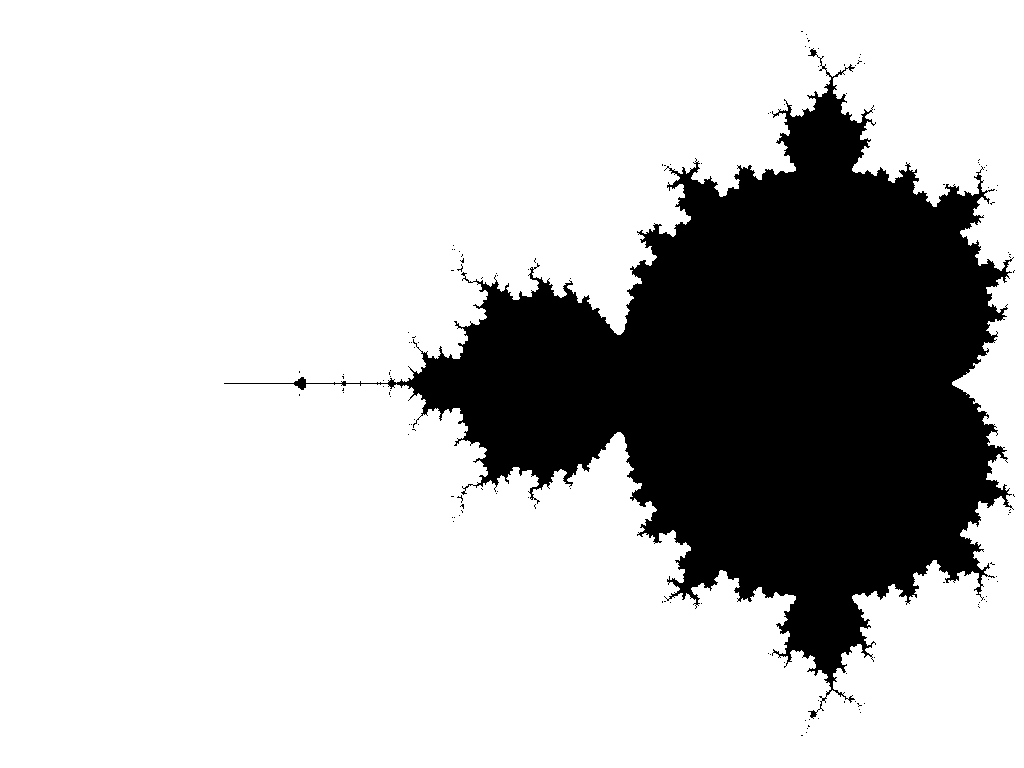
\includegraphics[width=0.7\textwidth]{figures/Mandelbrot_black.png}
  \caption{Манделбротов скуп над $c_r \in [-2.5, 1.0]$, $c_i \in [-1.25, 1.25]$}
  \label{fig:mandelbrot-set}
\end{figure}

$M$ поседује неколико својстава која су директно важна за његово рендеровање, сва
видљива на слици~\ref{fig:mandelbrot-set}. Прво, ограничен је. Ако је $|c| > 2$, низ из
једначине~\ref{eq:mandelbrot-iteration} гарантовано дивергира, тако да $M$ у целости
лежи унутар диска $|c| \leq 2$. Ово следи јер, чим постане $|z_n| > 2$ и $|z_n| \geq
|c|$, сваки наредни корак удаљеност од координатног почетка умножава фактором већим од
$1$, тако да $|z_n|$ неограничено расте. Исти аргумент оправдава рано заустављање
итерације за било који пиксел чим $|z_n|$ пређе тај праг, уместо бесконачног
итерирања. Друго, $M$ је повезан. Упркос томе што визуелно делује као скуп неповезаних
„острва'', свака тачка скупа може се повезати са сваком другом тачком путем који остаје
унутар $M$, што су Дуади и Хабард доказали кроз униформизацију скупа спољашњим
зрацима. Треће, $M$ је самосличан у лабавом смислу. Његова граница садржи бесконачно
много малих, изобличених копија целог скупа, на сваком нивоу увећања, познатих као
сателитске или „мини-Манделброт'' копије. Управо због тога увећавање границе стално
открива нови детаљ, уместо да конвергира ка једноставној кривој. То је такође разлог
зашто је рендеровање дубоког увећања, одељак~\ref{sec:perturbation}, уопште занимљив
проблем, а не само рачунање исте слике на мањој размери. Најзад, иако је $M$
дводимензиона област равни, његова граница је фрактална крива Хаусдорфове димензије
тачно $2$. То што је крива толико „испуњавајућа'' у простору је, неформално речено,
разлог зашто је тест бекства близу границе нумерички деликатан и зашто су пиксели чија
класификација траје најдуже концентрисани управо тамо где слика има највише визуелног
детаља.

\section{Основе рендеровања алгоритмом бекства}
\label{sec:escape-time-basics}

Једначина~\ref{eq:mandelbrot-iteration} се на стварном рачунару не може итерирати
бесконачно, па рендерер мора тачан тест припадности да претвори у две практичне
апроксимације.

Прва је праг излаза (енг. \emph{bailout}). Уместо да се чека да $|z_n| \to \infty$,
итерација стаје чим $|z_n|$ пређе фиксни радијус бекства. Радијус од $2$ већ је
довољан да се гарантује да ће тачка дивергирати, истим аргументом коришћеним у
одељку~\ref{sec:mandelbrot-definition}, па је сваки већи радијус безбедан, мада
понекад непотребан, избор. Рендерери који желе глађе бојење често намерно користе
већи радијус бекства, по цену неколико додатних итерација по пикселу који побегне.
Друга апроксимација је максималан број итерација. Пиксел који не побегне до достизања
тог ограничења третира се као да припада скупу, иако би нешто виши лимит на крају можда
показао да и он бежи. Подизање тог ограничења чини слику тачнијом, посебно близу
границе и на дубоком увећању, али и сваки пиксел који никада не побегне, типично
већина слике при великом увећању, чини сразмерно скупљим за рендеровање. Број
извршених итерација стога је веома неуједначен по слици. Пиксели далеко од $M$ бегају
готово тренутно, пиксели дубоко унутар скупа извршавају пуно ограничење итерација, а
пиксели близу границе могу непредвидиво учинити и једно и друго. Ова неуравнотеженост
оптерећења главни је разлог зашто наивна паралелизација по пикселу лоше ради, и то је
основни проблем који оптимизације у глави~\ref{ch:algorithms} и распоређивач у
глави~\ref{ch:scheduler} заобилазе.

Претварање сировог броја итерација у слику такође захтева пажњу. Директно мапирање
целобројног броја итерација у боју ствара видљиво пругање, оштре прстенове тамо где
се број мења за један, уместо глатког прелаза. Стандардно решење је глатко, или
„нормализовано'', бојење, које користи вредност $z_n$ у тренутку бекства за
израчунавање разломљеног броја итерација
\begin{equation}
  \label{eq:smooth-coloring}
  \nu = n + 1 - \frac{\log \log |z_n|}{\log 2},
\end{equation}
тако да суседни пиксели који су побегли, рецимо, након $41{,}3$ и $41{,}7$ итерација
добију видљиво различите, интерполиране боје, уместо да буду сврстани у исту траку.
Опсег вредности $\nu$ присутних у кадру потпуно се мења са нивоом увећања и локацијом.
Добро мапирање $\nu$ у палету боја обично такође захтева корак нормализације, на
пример изједначавање хистограма. Тиме се обезбеђује да се доступни унос палете троше
тамо где слика заиста има детаље, а не на бројеве итерација који се у том конкретном
кадру једва јављају.

\begin{figure}[H]
  \centering
  
\includegraphics[width=\textwidth]{figures/sr/escape-time-banding.png}
  \caption{Иста гранична област обојена сировим целобројним бројем итерација и глатким
  бројем из једначине~\ref{eq:smooth-coloring}. Прстенови на левој слици настају
  понављањем палете једном по целој итерацији. Десна слика пролази кроз исту палету,
  али интерполира унутар сваког прстена.}
  \label{fig:escape-time-banding}
\end{figure}

\chapter{Алгоритми рендеровања}
\label{ch:algorithms}

\section{Основна скаларна варијанта алгоритма бекства}
\label{sec:baseline-scalar}

Основна варијанта рендерера директна је, невекторизована имплементација итерације из
једначине~\ref{eq:mandelbrot-iteration}: један комплексан број типа \kod{f64} по
пикселу, један пиксел у једном тренутку. Две ствари је разликују од уџбеничке петље, и
обе су важне за то шта „основна варијанта'' значи у остатку ове главе. Прво, пре него
што уопште почне итерирање, извршавају се аналитички тестови раног изласка из
одељка~\ref{sec:early-exit}, тако да основна варијанта већ искључује два највећа
унутрашња дела скупа из петље итерације. Свака касније описана оптимизација у овој
глави мери се у односу на основну варијанту која већ садржи овај тест, а не у односу на
наивну петљу без икаквих пречица. Друго, корак ажурирања $z_{n+1} = z_n^2 + c$ записан
је као једна спојена инструкција множења и сабирања (енг. \emph{fused multiply-add}), а не
као одвојено множење и сабирање, тако да хардвер извршава један корак заокруживања
уместо два.

Сам тест бекства користи радијус успостављен у одељку~\ref{sec:escape-time-basics},
$|z_n|^2 > 4$, проверен као поређење квадрата како би се избегло вађење квадратног
корена у свакој итерацији. Поред прага излаза, рендерер извршава детекцију циклуса у
Брентовом стилу \cite{brent1980}. На сваких неколико итерација чува тренутну вредност
$z_n$, а у каснијим итерацијама је пореди са том сачуваном вредношћу. Ако се орбита
врати на удаљеност мању од $10^{-20}$ од ње, тачка се сматра периодичном и одмах се
класификује као да припада скупу, без чекања на \kod{max\_iter}. Интервал поређења
почиње на $8$ итерација и удвостручује се после сваке провере, до горње границе од
$512$. На овај начин провера се често извршава док постоји велика шанса да се исплати
рано, а ретко касније, када је мало вероватно да ће се активирати и када би иначе само
додавала непотребан трошак по итерацији. Ово хвата циклусе које кардиоидни и балонски
тестови пропуштају. Ти тестови су затворени облик за два највећа дела скупа. Граница,
међутим, садржи бесконачно много мањих периодичних делова, видљивих мањих балона и
ситних сателитских копија из одељка~\ref{sec:mandelbrot-definition}, које Брентов
метод и даље може генерички да ухвати, без унапред познатог облика.

Посао се дели по језгрима процесора у податковно-паралелним блоковима редова, а сама
петља по пикселима не садржи ниједно дељење или тригонометријску операцију по пикселу.
Пресликавање координата пиксела у комплексан број своди се, једном по кадру, на четири
константе, почетак и корак за реални и имагинарни део, тако да је координата сваког
пиксела удаљена један корак спој-множи-сабери од претходне. На референтној машини
коришћеној кроз цео овај рад, глава~\ref{ch:methodology}, ова основна варијанта
одржава пропусност од отприлике $195$ до $239$ милиона пиксела у секунди, за
резолуције од $800\times600$ до $3840\times2160$, за Манделбротов скуп при $1000$
итерација. Пропусност је практично константна у односу на резолуцију, што се и очекује
за посао чија цена по пикселу не зависи од величине слике око њега.

Листинг~\ref{lst:mandelbrot-scalar} показује ово језгро: позив теста затвореног
облика на самом почетку, а затим петљу итерације са Брентовом детекцијом циклуса,
описаном текстуално изнад.

\noindent\begin{minipage}{\linewidth}
\lstinputlisting[language=Rust, numbers=none,
  caption={Скаларна \kod{f64} итерација Манделбротовог скупа, референтна
  имплементација из које су SIMD, CUDA и WGSL кернели алгебарски изведени
  (\kod{src/fractal/kernels/mandelbrot.rs}).},
  label={lst:mandelbrot-scalar}]{listings/mandelbrot_scalar.rs}
\end{minipage}

\section{SIMD векторизација}
\label{sec:simd}

Скаларна петља из одељка~\ref{sec:baseline-scalar} рачуна итерацију једног пиксела у
једном тренутку, иако модерни процесори могу применити исту аритметичку операцију на
неколико вредности у једној инструкцији. SIMD кернели рендерера замењују скаларно
ажурирање $z_{n+1}=z_n^2+c$ истим ажурирањем примењеним на неколико пиксела
истовремено, спакованих у један векторски регистар: \kod{f64x4} са четири \kod{f64}
траке (енг. \emph{lanes}) и \kod{f32x8} са осам \kod{f32} трака. Који ће се користити
зависи од дубине увећања, преко истог прага од $10^6$ који се кроз цео овај рад
користи за избор између \kod{f32} и \kod{f64}. Испод те границе рендерер користи шири
и јефтинији \kod{f32x8} кернел. Изнад ње, приближно седам децималних цифара
прецизности које нуди \kod{f32} више нису довољне да разликују суседне пикселе, па се
прелази на \kod{f64x4}.

Векторизација петље алгоритма бекства уводи проблем ког скаларна петља нема. Различите
траке беже при различитом броју итерација, али SIMD инструкција примењује исту
операцију на све траке истовремено, тако да ниједна трака сама по себи не може рано да
стане. Кернели ово решавају маском активних трака, бит-узорком по траци, свих
јединица или свих нула, која се са ажурирањем комбинује бит-по-бит операцијом И
(AND). Чим $|z_n|^2$ одређене траке пређе радијус бекства, бележе се њена итерација
бекства и вредност $z_n$, а маска ту траку искључује, тако да даља ажурирања за њу
постају без ефекта, док остале траке настављају. Петља стаје тек када све траке побегну
или се достигне \kod{max\_iter}.

Трећи кернел, коришћен само за Манделбротов скуп, иде корак даље тако што покреће два
независна ланца \kod{f32x8} упоредо, шеснаест пиксела по кораку уместо осам. Два ланца
су иначе идентична. Поента је паралелизам на нивоу инструкција, а не додатна ширина
вектора. Модерни процесори могу имати неколико спојених инструкција множења и сабирања
у лету истовремено, ако постоји други, независан ланац посла који попуњава цевовод док
се резултат првог ланца још увек рачуна. Измерено на резолуцији $1920\times1080$ за
Манделбротов скуп при $1000$ итерација, кернел са два ланца рендерује кадар за
$4.25\,\mathrm{ms}$, наспрам $4.62\,\mathrm{ms}$ за једноструки \kod{f32x8} кернел,
$6.04\,\mathrm{ms}$ за \kod{f64x4} и $8.17\,\mathrm{ms}$ за скаларну основну варијанту,
што је убрзање од $1.92\times$ у односу на скаларну варијанту, од чега само око $8\%$
потиче од самог другог ланца. То што је додатни добитак од паралелизма на нивоу
инструкција мали није изненађење када се узме у обзир одељак~\ref{sec:early-exit}.
Кардиоидни и балонски тестови већ уклањају велики део унутрашњих пиксела пре него што
„врућа'' петља уопште крене, остављајући мање кашњења које би други ланац могао да
сакрије. Једно мерење током бенчмаркинга такође је показало да се два наизглед
идентична, поновљена мерења истог кернела разликују за више од половине.
Глава~\ref{ch:methodology} се на ово враћа као подсетник да је једно мерење бенчмарка
само шум све док се не понови.

Листинг~\ref{lst:mandelbrot-simd} показује маску \kod{active} из \kod{f32x8}
кернела описану изнад: провера \kod{just\_escaped} бележи која поља су управо
побегла бит-по-бит операцијом И, а ажурирање \kod{active} одмах затим искључује та
поља из маске тако да их даља ажурирања више не дотичу, иако цео вектор наставља
да се рачуна до краја петље.

\noindent\begin{minipage}{\linewidth}
\lstinputlisting[language=Rust, numbers=none,
  caption={Маска активних трака у \kod{f32x8} Манделбротовом кернелу
  (\kod{src/fractal/kernels/mandelbrot.rs}).},
  label={lst:mandelbrot-simd}]{listings/mandelbrot_simd.rs}
\end{minipage}

\section{Геометријски тестови раног изласка}
\label{sec:early-exit}

Две области Манделбротовог скупа довољно су велике и довољно једноставног облика да се
припадност може директно тестирати из $c$, без икаквог итерирања, стандардно убрзање
описано у \cite{peitgensaupe1988}. Главна кардиоида, највећа компонента, представља
слику јединичне кружнице под пресликавањем $c = \tfrac{1}{2}e^{i\theta} -
\tfrac{1}{4}e^{2i\theta}$. Еквивалентно, уз ознаку $q = (c_r - 0.25)^2 + c_i^2$, тачка
припада кардиоиди тачно када
\begin{equation}
  \label{eq:cardioid-test}
  q \, (q + c_r - 0.25) < 0.25 \, c_i^2 .
\end{equation}
Балон периода 2, велика кружна компонента прикачена на леву страну кардиоиде, тачан је
диск, $(c_r + 1)^2 + c_i^2 < 0.0625$, полупречника $0.25$ са центром у $c = -1$. Оба
теста су тачни алгебарски идентитети, а не апроксимације, тако да свака тачка коју они
класификују као унутрашњу то заиста и јесте, и може јој се директно доделити
\kod{max\_iter}, без икакве итерације.

Рендерер такође тестира два балона периода 3, следеће по величини унутрашње
компоненте, прикачене на кардиоиду изнад и испод балона периода 2. Они немају тако чист
затворени облик као кардиоида, али је сваки од њих ипак добро апроксимиран диском, са
центром близу $c \approx (-0.122561, \pm0.744862)$ и полупречником $\approx 0.073715$.
Поређење квадрата растојања са квадратом полупречника поново избегава вађење квадратног
корена. После периода $3$, граница наставља без краја да производи мање балоне и
сателитске копије, одељак~\ref{sec:mandelbrot-definition}, па више нема смисла ручно
изводити затворени тест за сваки од њих. Мање периодичне компоненте уместо тога хвата
генерички механизам детекције циклуса, већ уграђен у основну варијанту,
одељак~\ref{sec:baseline-scalar}.

Ова три теста извршавају се прво, пре петље итерације, за сваки пиксел у сваком
кернелу у овој глави, скаларном и SIMD подједнако. Тестови за кардиоиду и период 2
директно се векторизују, пошто су то само аритметичке операције над SIMD тракама. Тест
за период 3, чији се центри дискова не векторизују тако чисто, уместо тога се
процењује по траци у скаларној прецизности, и то само за пикселе које прва два теста
нису већ разрешила. Главна кардиоида и балон периода 2 два су највеће области скупа по
површини. Само овај тест стога обухвата велики удео пиксела који би иначе трчали до
\kod{max\_iter} не радећи ништа корисно, управо оних „тешких'' пиксела
идентификованих као главни извор неуравнотежености оптерећења у
одељку~\ref{sec:escape-time-basics}.

\begin{figure}[H]
  \centering
  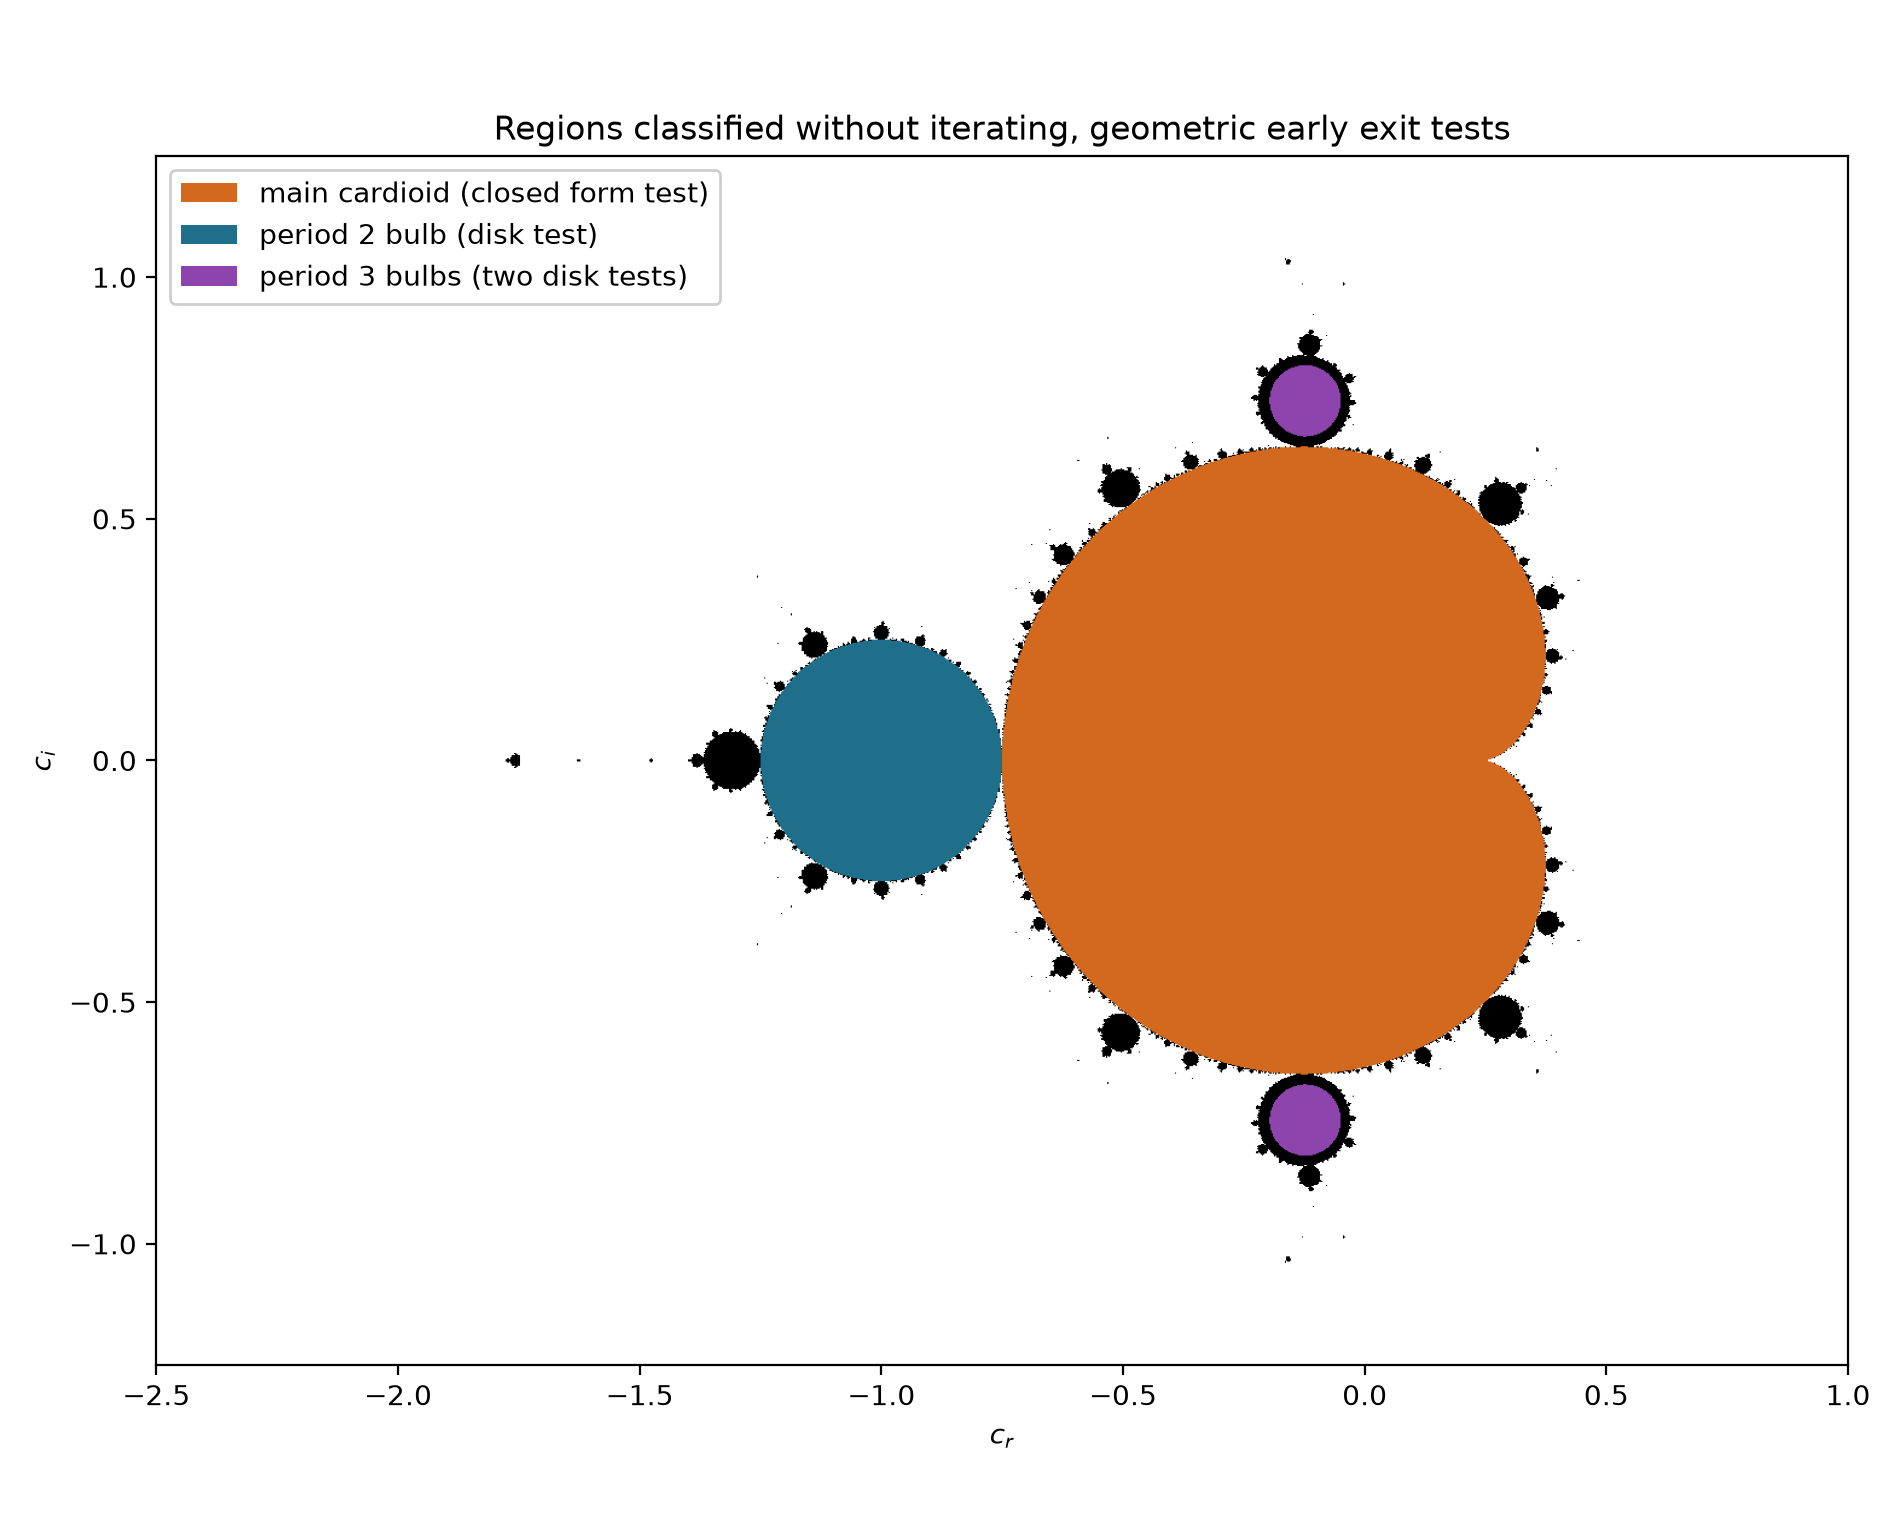
\includegraphics[width=0.85\textwidth]{figures/alg-early-exit-regions.png}
  \caption{Три области затвореног облика приказане на рендеру целог кадра
  Манделбротовог скупа: главна кардиоида, балон периода 2 и два балона периода 3.
  Сваком пикселу унутар осенчене области директно се додељује \kod{max\_iter}, без
  икакве итерације. Свуда другде, укључујући и мање сателитске балоне видљиве дуж
  границе, и даље се извршава пуна петља.}
  \label{fig:early-exit-regions}
\end{figure}

\section{Мариани-Силвер подела границе}
\label{sec:mariani-silver}

Тестови из одељка~\ref{sec:early-exit} у затвореном облику класификују појединачне
пикселе као унутрашње. Мариани-Силвер подела \cite{peitgensaupe1988} уместо тога
користи чињеницу да велике области \emph{спољашњости} скупа, далеко од границе, такође
деле исти број итерација бекства са својим суседима. Алгоритам затим покушава да
открије и попуни такве области без израчунавања сваког пиксела унутар њих.

За дати правоугаоник слике, алгоритам рендерује само његову ивицу: горњи и доњи ред и
леву и десну колону. Ако сви пиксели ивице имају исту вредност, правоугаоник се сматра
униформним и цела његова унутрашњост попуњава се том вредношћу, без икаквог
додиривања пиксела унутар ње. Ако ивица није униформна, правоугаоник је премали да би
та претпоставка била безбедна. Уместо тога, дели се на два дела дуж своје дуже осе,
тако да оба дела остану ближа квадрату него да настану дуге, издужене траке, и исти
тест се рекурзивно примењује на сваки од њих. Ово се наставља све до минималне
величине од $2\times2$ пиксела, испод које подела више не исплати сама себе, па се
преостали пиксели једноставно рачунају директно. Суседни правоугаоници деле ивицу, па
се бафер кадра унапред попуни сигналном (енг. \emph{sentinel}) вредношћу, а пиксел ивице
који је већ израчунат од стране суседног правоугаоника никада се не рачуна поново.

\begin{figure}[H]
  \centering
  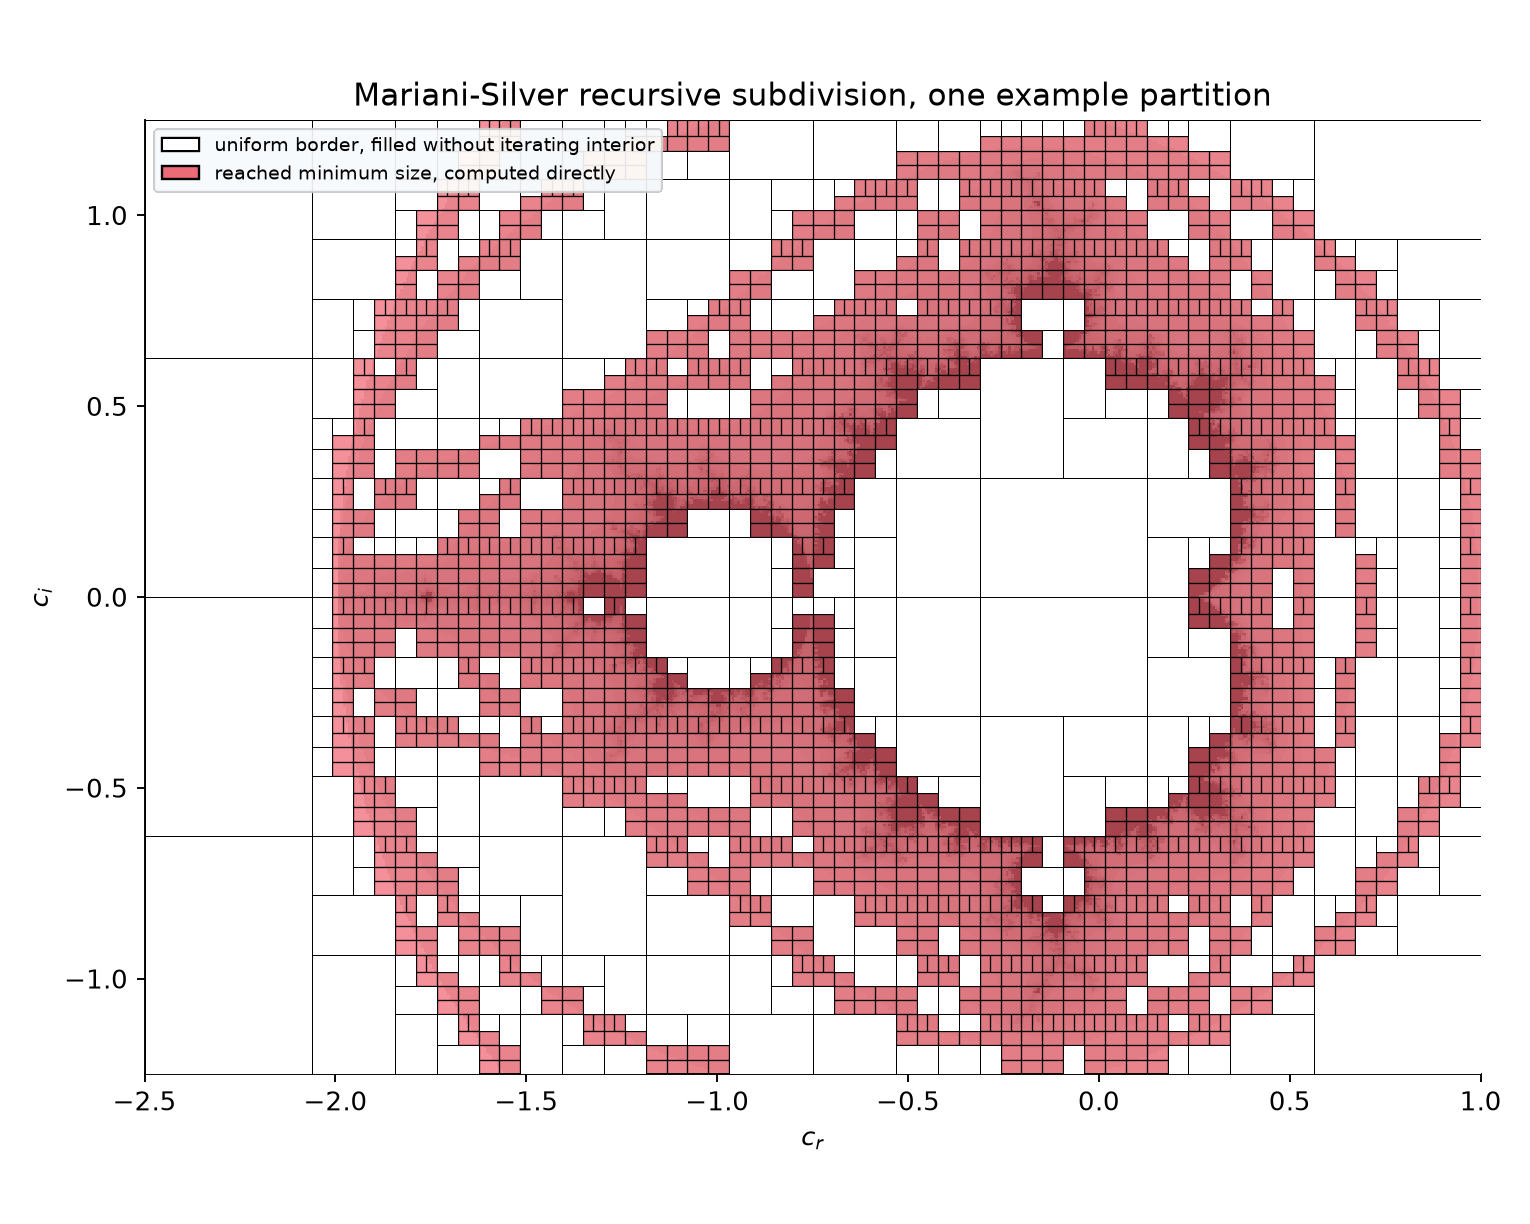
\includegraphics[width=0.85\textwidth]{figures/alg-mariani-silver-example.png}
  \caption{Пример поделе приказан на рендеру целог кадра Манделбротовог скупа;
  минимална величина овде је ради видљивости подигнута на $6\times6$ пиксела, док сам
  рендерер стаје на $2\times2$. Бели правоугаоници имали су униформну ивицу и попуњени
  су без додиривања своје унутрашњости. Црвени правоугаоници достигли су минималну
  величину и израчунати су директно.}
  \label{fig:mariani-silver-example}
\end{figure}

Претпоставка о униформној ивици није строго загарантована. У принципу, танак нит
пиксела различите вредности могао би да прође кроз унутрашњост правоугаоника, а да
никада не додирне његову ивицу, у ком случају би корак попуњавања преко њега прешао
бојом. У пракси је ово довољно ретко, а визуелна цена довољно мала, да алгоритам ово
прихвата као познату, ограничену апроксимацију ризика, уместо да се експлицитно штити
од ње.

Друга варијанта укључује и процену растојања из одељка~\ref{sec:dem}. Уместо да само
проверава да ли је ивица униформна, она такође проверава да ли је свако теме
правоугаоника даље од границе скупа него што износи сопствена дијагонала
правоугаоника, скалирана подесивим сигурносним фактором $k$. Ако јесте, зна се да је
цео правоугаоник довољно далеко од сваког граничног детаља да је билинеарна
интерполација између четири вредности у теменима визуелно неразлучива од израчунавања
сваког пиксела. Правоугаоник се тада тако попуњава, уз проверу исправности да се
глатки бројеви итерација у теменима не разликују за више од $2.0$. Ова провера је
важна јер би билинеарно попуњавање преко области у којој се основна функција брзо
мења видљиво погрешно рендеровало ту област.

\section{Метод процене растојања}
\label{sec:dem}

Метод процене растојања \cite{peitgensaupe1988} одговара на другачије питање од теста
бекства: не колико итерација треба да $c$ побегне, већ колико је $c$ удаљено од
границе скупа. Строго математичко оправдање ове величине долази из теорије потенцијала
спољашњости скупа \cite{milnor2006}. Процена следи из праћења, паралелно са обичном
орбитом $z_{n+1} = z_n^2 + c$, њеног извода по $c$.
\begin{equation}
  \label{eq:dem-derivative}
  z_0 = 0, \quad \frac{dz_0}{dc} = 0, \qquad
  z_{n+1} = z_n^2 + c, \quad \frac{dz_{n+1}}{dc} = 2 z_n \frac{dz_n}{dc} + 1,
\end{equation}
добијеног диференцирањем саме итерације члан по члан. Ако орбита побегне у итерацији
$n$, растојање од $c$ до најближе тачке границе приближно износи
\begin{equation}
  \label{eq:dem-distance}
  d \approx \frac{|z_n| \, \ln |z_n|}{|dz_n/dc|} .
\end{equation}

Ово је стандардан резултат за процену спољашњег растојања код фрактала заснованог на
алгоритму бекства, не нешто специфично за овај рендерер. Оно што јесте специфично за
овај рендерер јесте начин на који се та вредност користи. Уместо да покреће посебан
режим анти-алијасинга или контурног рендеровања, $d$ се користи тачно једном: као
тест одсецања унутар DEM-проширене Мариани-Силвер варијанте из
одељка~\ref{sec:mariani-silver}. За правоугаоник чија су сва четири темена даља од
границе него што износи сопствена дијагонала правоугаоника гарантовано је да не садржи
ниједан фини гранични детаљ, па се безбедно може попунити интерполацијом уместо
итерирањем пиксел по пиксел. Пошто се $dz_n/dc$ акумулира кроз једну додатну
комплексну операцију спој-множи-сабери по итерацији, поред обичне орбите, процена
растојања готово да се добија бесплатно уз извршавање теста бекства који би се
свакако десио. Стварна уштеда долази од тога колико посла пиксел-по-пиксел тест
одсецања омогућава Мариани-Силвер алгоритму да прескочи, а не од тога што је сама
процена јефтина посматрана изоловано.

\section{Теорија пертурбације}
\label{sec:perturbation}

Сваки до сада описани кернел директно итерира $c$ у типу \kod{f64} или \kod{f32}, што
престаје да функционише чим је увећање толико дубоко да се вредности $c$ суседних
пиксела разликују мање него што аритметика двоструке тачности може да разлучи. Та
граница се достиже далеко пре режима дубоког увећања који самослична граница из
одељка~\ref{sec:mandelbrot-definition} чини занимљивим. Теорија пертурбације
\cite{martin2013superfractalthing} ово заобилази итерирањем \emph{разлике}, а не
апсолутне вредности. Једна референтна орбита високе прецизности $Z_n$ рачуна се
једном, за једну референтну тачку близу центра приказа. Сваки други пиксел $c =
c_{\mathrm{ref}} + \delta c$ затим се рендерује директним итерирањем много мање
величине $\delta_n = z_n - Z_n$.
\begin{equation}
  \label{eq:perturbation}
  \delta_{n+1} = 2 Z_n \delta_n + \delta_n^2 + \delta c ,
\end{equation}
добијене одузимањем рекурзије саме референтне орбите од рекурзије пиксела. Пошто
$\delta_n$ остаје мало за већину пиксела близу референтне тачке, оно се може итерирати
у обичном \kod{f64} чак и тамо где би за представљање одговарајућег $z_n$ била
потребна далеко већа прецизност. Ово значи да се скупи посао високе прецизности из
одељка~\ref{sec:precision} плаћа једном по кадру, а не једном по пикселу.

\begin{figure}[H]
  \centering
  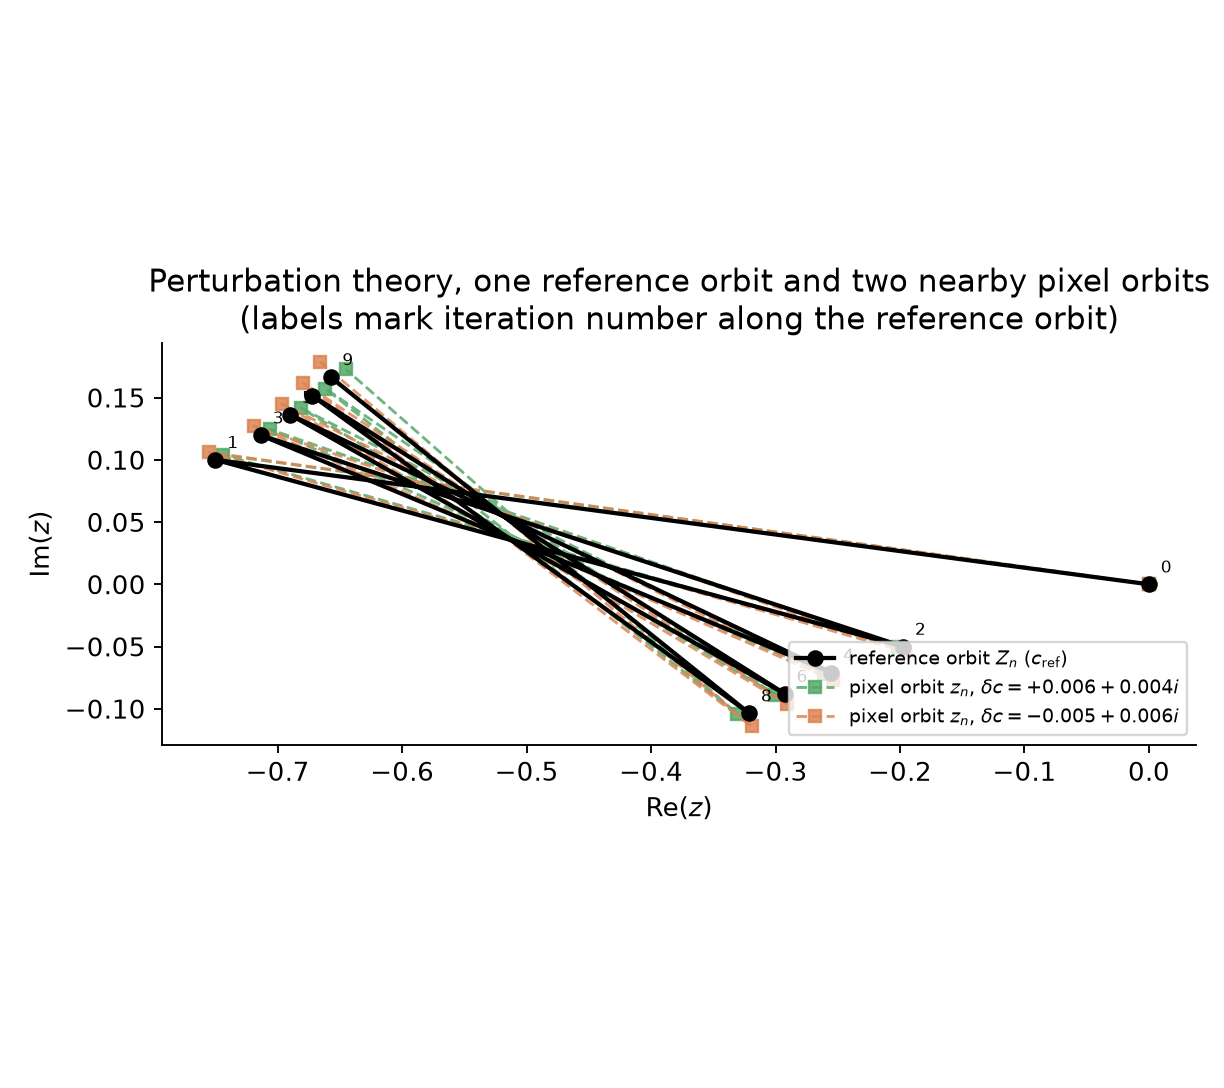
\includegraphics[width=0.7\textwidth]{figures/perturbation-schematic.png}
  \caption{Стварна референтна орбита у $c_{\mathrm{ref}}=-0.75+0.1i$, тачки „долине
  морских коњица'' коју користи и одељак~\ref{sec:bench-viewports}, заједно са две
  орбите пиксела удаљене за мало $\delta c$. Све три орбите остају близу једна другој
  за приказане итерације, што је управо оно што омогућава да $\delta_n$ буде
  представљено у обичном \kod{f64}, док сама $Z_n$ носи проширену прецизност.}
  \label{fig:perturbation-schematic}
\end{figure}

Ово не важи за пикселе чија орбита превише одлута од референце. Чим $|\delta_n|$
нарасте до незанемарљивог дела $|Z_n|$, апроксимација на коју се метод ослања престаје
да важи, догађај обично назван \emph{глич} (енг. \emph{glitch}). Рендерер ово открива
поређењем $|\delta_n|^2$ са малим фиксним делом $|Z_n|^2$ и означава пиксел чим се та
граница пређе. Обична варијанта за сваки означени пиксел једноставно прелази на тачан
скаларни кернел из одељка~\ref{sec:baseline-scalar}, што је увек тачно, али поново
плаћа пуну цену по пикселу управо за оне пикселе које је пертурбација требало да
избегне директно рачунати. \emph{Ребазирање} (енг. \emph{rebasing}) \cite{heilandallen2021deepzoom}
избегава већину тог прелаза без потребе за другом референтном орбитом. Кад год орбита
пиксела поново прође близу координатног почетка, чим $|z_n|^2$ падне испод
$|\delta_n|^2$, или кад сачувана референтна орбита истекне, тренутна вредност $z_n$
једноставно се усваја као нова, локална делта од $0$, и итерација се од те тачке даље
наставља у односу на исту референтну орбиту, поново користећи једну унапред
израчунату орбиту као да је ту бесплатно израчуната свежа референца. Рендеровање са
\emph{више референци} (енг. \emph{multi-reference}) иде и корак даље. Оно рендерује цео
кадар у односу на једну референцу, обележава сваки глич-пиксел, а затим рачуна нову
референцу центрирану на први још увек глич-пиксел, пошто се гличеви просторно групишу,
суседни пиксели теже да заједно одлутају од дате референце, понављајући овај
поступак до $8$ референтних орбита пре него што одустане и пређе на тачан кернел за
све што остане нерешено.

Директним мерењем, рендеровање пертурбацијом не доноси добитак у пропусности. У
испитаном опсегу увећања оно рендерује спорије од директног кернела који замењује, јер
тај опсег никада не достиже дубину на којој \kod{f64} стварно постаје недовољан, тако
да је машинерија пертурбације чист додатни трошак изнад аритметике коју би директни
кернел ионако сам могао да обави.

Листинг~\ref{lst:perturb-rebase} показује \kod{perturb\_mandelbrot\_rebase}, варијанту
са ребазирањем. Ажурирање \kod{er}/\kod{ei} је директан код рекурзије из
једначине~\ref{eq:perturbation}, а провера \kod{if zn\_sq < er * er + ei * ei || m ==
orbit.len} је сам услов ребазирања: чим квадрат модула тренутне позиције орбите
падне испод квадрата модула саме делте, или чим се референтна орбита потроши,
тренутна позиција $(az, bz)$ постаје нова делта, а $m$ се враћа на нулу.

\noindent\begin{minipage}{\linewidth}
\lstinputlisting[language=Rust, numbers=none,
  caption={Итерација пертурбације са ребазирањем
  (\kod{src/fractal/perturbation/perturbation\_theory.rs}).},
  label={lst:perturb-rebase}]{listings/perturb_rebase.rs}
\end{minipage}

\section{Апроксимација степеним редом}
\label{sec:series-approximation}

Итерација пертурбације из одељка~\ref{sec:perturbation} и даље извршава по једно
ажурирање $\delta_n$ по пикселу по итерацији. Апроксимација степеним редом
\cite{martin2013superfractalthing, heilandallen2021deepzoom} покушава у потпуности да
прескочи првих неколико стотина итерација тог посла, за пикселе довољно блиске
референтној орбити да је њихово рано понашање предвидиво у затвореном облику.

Уврштавањем претпоставке степеног реда $\delta_n \approx A_n \delta c + B_n \delta c^2
+ C_n \delta c^3 + D_n \delta c^4$ у рекурзију пертурбације, једначина~\ref{eq:perturbation},
и изједначавањем степена $\delta c$ добија се рекурзија за саме коефицијенте,
израчуната једном, заједно са референтном орбитом.
\begin{align}
  \label{eq:sa-coefficients}
  A_{n+1} &= 2 Z_n A_n + 1, &
  B_{n+1} &= 2 Z_n B_n + A_n^2, \\
  C_{n+1} &= 2 Z_n C_n + 2 A_n B_n, &
  D_{n+1} &= 2 Z_n D_n + \left(2 A_n C_n + B_n^2\right).
\end{align}
Све док чланови трећег и четвртог реда остају занемарљиви у односу на водећи члан за
најгори случај $\delta c$ у кадру, теме приказа најудаљеније од референтне тачке,
ред је ваљана замена за директну итерацију. Рендерер прати последњу итерацију у којој
то још важи, за сваки пиксел директно процењује ред у тој итерацији, а затим наставља
обичну итерацију пертурбације од те тачке, уместо од нулте итерације.

На сцени за бенчмарк коришћеној изнад за пертурбацију, испоставља се да је прескочиви
префикс кратак. Он износи свега неколико десетина итерација од хиљаду, предност од
један до три процента, а не велики почетни прескок који апроксимација степеним редом
омогућава на већим дубинама.

\section{Нумеричка прецизност за дубоко увећање}
\label{sec:precision}

Теорија пертурбације, одељак~\ref{sec:perturbation}, помера проблем прецизности
уместо да га уклања. Делте пиксела могу остати у \kod{f64}, али једна референтна
орбита у односу на коју се оне рачунају и даље мора да прати апсолутну позицију у
комплексној равни, а на екстремном увећању тој позицији је потребно више од приближно
$53$ бита мантисе које нуди \kod{f64} да би се разликовала од суседних. Уместо
увођења библиотеке за аритметику произвољне прецизности, рендерер представља реалан
број проширене прецизности на начин Декерове класичне „double-double'' технике
\cite{dekker1971}: као неевалуирани пар обичних вредности типа \kod{f64}, $(hi,
lo)$, уз инваријанту да је $|lo|$ највише пола јединице последњег места у $hi$.
Стварна вредност је тачан збир $hi + lo$, који се никада заправо не рачуна као један
број покретног зареза. Ова „double-double'' репрезентација даје приближно $106$ бита
мантисе, двоструко више него \kod{f64}, док се свака појединачна операција над њом и
даље извршава као обична хардверска аритметика покретног зареза.

Два градивна елемента су Кнутов \kod{TwoSum} \cite{knuth1997seminumerical}, кратак
низ операција без гранања који рачуна $a+b$ заједно са тачном грешком заокруживања у
другом броју, и \kod{TwoProduct} \cite{ogitarumpoishi2005}, који исту тачну
декомпозицију грешке за множење добија директно из спојене инструкције множења и
сабирања. Он рачуна $p = a \times b$, а затим члан грешке као $a \times b - p$ у једној
спојеној инструкцији множења и сабирања, без потребе за посредним резултатом двоструке
ширине. Сабирање над типом пара сабира горње делове помоћу \kod{TwoSum}, увија оба
доња дела у резултујући члан грешке и поново нормализује другим позивом \kod{TwoSum}.
Множење рачуна тачан производ горњих делова помоћу \kod{TwoProduct}, додаје унакрсне
чланове $hi_a \cdot lo_b$ и $lo_a \cdot hi_b$ као обичне \kod{f64} производе, који су
већ довољно мали да им није потребан сопствени члан грешке, и на исти начин поново
нормализује.

Ова проширена прецизност користи се на тачно једном месту, при рачунању саме
референтне орбите, чим тражено увећање пређе фиксни праг од $10^{12}$, изнад ког
обичан \kod{f64} више није поуздан за ту орбиту. Свако ажурирање $\delta_n$ по пикселу
и даље се извршава у обичном \kod{f64} у односу на ту орбиту, скраћено назад из
репрезентације пара приликом чувања, пошто самим делтама никада није ни била потребна
додатна прецизност, само дељеној референци. Пошто се референтна орбита рачуна једном
по кадру, а не једном по пикселу, приближно двоструко већи аритметички трошак
double-double операција у односу на обичан \kod{f64} остаје занемарљив у односу на
укупно време кадра, чак и када је активан.

\section{Обилазак и локалност}
\label{sec:traversal-locality}

Сваки до сада описан алгоритам одлучује \emph{шта} да се израчуна за пиксел. Овај
одељак бави се редоследом \emph{којим} се пиксели посећују, као и потпуним избегавањем
поновног рачунања када претходни кадар већ садржи већи део одговора.

Рендерер дели кадар на квадратне плочице од $64 \times 64$ пиксела и расподељује траке
плочица по радним нитима процесора. Ова фиксна величина плочице уједно је и јединица
посла коју хибридни распоређивач из главе~\ref{ch:scheduler} шаље процесору и
графичком процесору. Унутар плочице, пиксели се могу посећивати у обичном редоследу по
редовима, или дуж Хилбертове криве \cite{hilbert1891}, рекурзивно дефинисане путање
која увек прелази на геометријски суседан пиксел и, за разлику од редоследа по
редовима, никада на крају реда не скаче назад преко целе ширине плочице. Хилбертов
редослед посете за плочицу генерише се једном преплитањем битова и ротирањем
квадраната, и поново се користи непромењен за сваку плочицу у кадру, тако да је цена
по пикселу само провера у табели, а не поновно рачунање криве.

\begin{figure}[H]
  \centering
  
\includegraphics[width=\textwidth]{figures/traversal-hilbert-vs-rowmajor.png}
  \caption{Редослед посете пиксела унутар једне плочице, редослед по редовима наспрам
  Хилбертове криве. Редослед по редовима на крају сваког реда скаче назад преко целе
  ширине плочице. Хилбертова крива никада не прави корак који није ка геометријски
  суседном пољу.}
  \label{fig:traversal-hilbert}
\end{figure}

Мотивација за испробавање Хилбертовог редоследа уопште јесте локалност кеша.
Узастопни пиксели дуж криве такође су просторно блиски на слици, па би, ако цео бафер
кадра не стане у кеш, то требало да значи мање избацивања него код обиласка по
редовима, који поново посећује околину реда тек након што прође кроз све остале редове
између. На хардверу за бенчмарк коришћеном у овом раду, тај очекивани добитак се не
јавља. Хилбертов обилазак мерљиво спорије рендерује од обичног редоследа по редовима
на свакој испитаној резолуцији, а стопа промашаја кеша последњег нивоа му је виша, а
не нижа. Најизгледније објашњење, испитано у глави~\ref{ch:results}, јесте да бафер
кадра на испитаним резолуцијама већ удобно стаје у кеш последњег нивоа процесора, уз
хардверско унапред дохватање (енг. \emph{prefetching}) које успешно ради на приступном
обрасцу по редовима, тако да преплитање битова по пикселу код Хилбертове криве постаје
чист додатни трошак, без преосталог проблема локалности који би требало да реши.
Другачији редослед обиласка, Мортоново или Z-индексирање \cite{morton1966}, користи се
на другом месту у овом рендереру, али на графичком процесору, а не на овде описаној
путањи плочица на процесору. Одељак~\ref{sec:gpu-traversal} описује како он одржава да
нити унутар једног GPU „warp''-а приступају блиској меморији.

Померање приказа (енг. \emph{panning}) уопште не мора да утиче на редослед обиласка, већ
само на количину обављеног посла. Када се приказ помери дуж једне осе, већина пиксела
претходног кадра поново се јавља на помереној позицији, уместо да их треба поново
рачунати. Рендерер копира део старог бафера који се може поново искористити на његову
нову позицију једним масовним копирањем меморије и рачуна само новооткривену траку
дуж ивице ка којој се приказ померио. Ово претвара поновно рачунање целог кадра у копирање плус рачунање сразмерно
растојању померања, не површини кадра, али само за померање дуж једне осе.
Истовремено хоризонтално и вертикално померање захтевало би преклапајуће копирање
поново искоришћених и новооткривених области, што масовно копирање не омогућава,
па се дијагонално померање рачуна директно, пошто делимично поновно коришћење
ионако не би уштедело посао.

\chapter{Имплементација на графичком процесору}
\label{ch:gpu}

\section{WebGPU кернели}
\label{sec:webgpu}

WebGPU је преносиво од два позадинска решења рендерера за графички процесор. Исти
компајлирани шејдер извршава се на сваком графичком процесору са Vulkan, Metal или
DirectX драјвером, по цену једног строгог ограничења. WGSL, шејдерски језик у који се
WebGPU компајлира, уопште нема тип \kod{f64}, тако да је сваки кернел у овом
позадинском решењу искључиво \kod{f32}. За разлику од позадинских решења за процесор и
CUDA, ово позадинско решење нема сопствени резервни механизам за дубоко увећање.
Остаје унутар истог прага увећања од $10^6$ који се кроз цео рад користи за брзу
путању \kod{f32}, а све изнад тог прага рендерује се на потпуно другом позадинском
решењу.

Унутар тог ограничења, WebGPU кернел блиско прати сопствене \kod{f32} кернеле
процесора. Извршава исте тестове за кардиоиду, период 2 и период 3 из
одељка~\ref{sec:early-exit}, уграђене директно у шејдер, и прескаче детекцију
периодичности на исти начин као SIMD кернели процесора, из истог разлога: Брентова
провера циклуса се не исплати уз додатно гранање на \kod{f32} гранулацији. Кернел за
Манделбротов скуп дели своју шејдерску датотеку са осталим типовима фрактала у
рендереру, које се бирају у реалном времену помоћу целобројног поља у малом
униформном баферу параметара приказа и рендеровања, отпремљеном једном по кадру. Две
улазне тачке деле овај код кернела. Једна покреће по једну нит по пикселу за цео кадар
у редоследу по редовима, у радним групама од $16 \times 16$. Друга уместо тога чита
отпремљени низ дескриптора плочица и користи позицију сваке радне групе у
распоређивању да изабере једну, проверавајући границе локалне позиције сваке нити у
односу на ширину и висину те плочице пре уписивања на њену стварну позицију у баферу
кадра. Кроз ову другу улазну тачку шаље своје позиве GPU радник хетерогеног
распоређивача (глава~\ref{ch:scheduler}), пошто му је потребно да у једном позиву
рендерује произвољан скуп плочица које бира распоређивач, а не цео кадар.

Посебан шејдер обрађује рендеровање пертурбацијом. Он отпрема референтну орбиту
(одељак~\ref{sec:perturbation}) као два \kod{f32} низа за реални и имагинарни део,
заједно са њеним центром, и итерира исту рекурзију делте, једначина~\ref{eq:perturbation},
коју користе и кернели на процесору, прелазећи на директну \kod{f32} евалуацију
Манделбротовог скупа при гличу или када отпремљена орбита истекне. Не врши ребазирање и
не покушава поново са другом референцом. За разлику од три варијанте на процесору,
WebGPU пертурбација користи само једну референцу. Ребазирање и вишеструке референце
додале би контролни ток који мора идентично да се извршава кроз сваку нит у радној
групи да би остао јефтин на графичком процесору, а процењено је да то није вредно за
позадинско решење чији је домет ионако ограничен на \kod{f32}.

Враћање резултата хосту кошта више него његово израчунавање. Кернел уписује у
складишни бафер на страни графичког процесора. Копирање са уређаја на уређај затим га
премешта у други бафер означен за мапирање ка хосту, који се асинхроно мапира и чека,
пре него што се његов садржај копира у свеже алоциран бафер на хосту. При резолуцији
$1920\times1080$, увећању $1$, \kod{max\_iter}~$=1000$, сам кернел се извршава за
$0.29\,\mathrm{ms}$, али цео кадар траје $2.26\,\mathrm{ms}$. Читање назад чини
отприлике $90\%$ тога.

\section{CUDA позадинско решење}
\label{sec:cuda}

CUDA позадинско решење директно циља дискретни NVIDIA графички процесор, уместо да
пролази кроз слој преносивости. Кернел се унапред компајлира помоћу \kod{nvcc},
циљајући архитектуру \kod{sm\_86}, која одговара RTX 3050 генерације Ampere на којој
се овај рад бенчмаркује, а резултујући PTX уграђује се у компајлирани извршни фајл,
тако да ништа не мора да се компајлира у реалном времену. Две компајлерске опције
вреди посебно истаћи. Једна задржава денормализоване бројеве покретног зареза,
\kod{--ftz=false}, пошто их формула глатког бојења, одељак~\ref{sec:escape-time-basics},
захтева ради тачности близу прага бекства. Друга у потпуности искључује сажимање
спојеног множења и сабирања, \kod{--fmad=false}. Тај други избор је слика у огледалу
кернела на процесору из одељка~\ref{sec:baseline-scalar}, који FMA \emph{укључује}
ради брзине и прихвата разлику од једног корака заокруживања у односу на одвојено
множење и сабирање. Овде је искључен како би CUDA-ина аритметика заокруживала потпуно
исто као и аритметика процесора, жртвујући мало пропусности графичког процесора за
слике које су бит-по-бит идентичне између позадинских решења, што је важно када се та
два директно пореде (глава~\ref{ch:results}).

За разлику од WebGPU позадинског решења, ово задржава своје подразумеване кернеле у
\kod{f64}, чиме постиже потпуни паритет са основном варијантом на процесору. Извршава
исте тестове за кардиоиду, период 2 и период 3, као и исту детекцију циклуса у
Брентовом стилу из одељка~\ref{sec:baseline-scalar}. Испод истог прага увећања од
$10^6$, коришћеног свуда другде у овом раду, преузимају посебни \kod{f32} кернели,
огледајући сопствено распоређивање прецизности процесора. Посебан кернел обрађује
пертурбацију, чувајући референтну орбиту и сваку делту по пикселу у \kod{f64}, за
разлику од искључиво \kod{f32} путање WebGPU позадинског решења. Он чак ни не прима
координате референтне тачке као аргумент. Пошто се орбита увек рачуна за сопствени
средишњи пиксел кадра, кернел реконструише $c_{\mathrm{ref}}$ директно из геометрије
самог кадра. Као и WebGPU позадинско решење, нема ребазирање нити поновни покушај са
другом референцом, а ниједно од два позадинска решења не користи double-double
аритметику из одељка~\ref{sec:precision}. Нивои увећања довољно дубоки да им је она
потребна у овој имплементацији и даље се рендерују искључиво на процесору.

Погрешно постављене заставице и погрешна политика прецизности нису хипотетички ризик.
Тест периода 3 у \kod{f32} кернелу за Манделбротов скуп некада је позивао \kod{f64}
верзију функције \kod{in\_period3\_bulb}, по логици да и сопствени \kod{f32} кернел
процесора на исти начин позива своју \kod{f64} проверу балона, а да се та провера
извршава само једном по пикселу, а не једном по итерацији, па не би требало да буде
важна. То резоновање важи на процесору, где \kod{f64} и \kod{f32} аритметика коштају
приближно исто. На овом графичком процесору не важи. Ampere извршава \kod{f64} на
отприлике $1/64$ пропусности \kod{f32}, тако да осам \kod{f64} операција, извршених
једном по пикселу, кошта колико и пропусност издавања инструкција за целу петљу од
хиљаду итерација у \kod{f32} која их следи. Аблациони тест који је мерио само кернел,
без преноса ка хосту, показао је да верзија са \kod{f64} провером ради за
$0.910\,\mathrm{ms}$, наспрам $0.452\,\mathrm{ms}$ након замене правим \kod{f32}
тестом балона, фактор два, потврђен директним прегледом компајлираног PTX-а. Осам
\kod{f64} инструкција преживело је у старом кернелу, а нула у новом. Исправка је
проверена као бит-по-бит идентична оригиналу, не само визуелно слична, рендеровањем
седам приказа изабраних да оптерете управо ону границу коју провера штити, укључујући
приказе центриране директно на луку периода 3 при нивоима увећања до прага прецизности
$10^6$, и поређењем сваког од $2{,}073{,}600$ пиксела. Ниједан се није разликовао, ни
у једном приказу. Остварени ефекат на потпуно рендерован кадар, укључујући пренос ка
хосту који доминира временом, био је смањење од $15$ до $19\%$ на свакој испитаној
резолуцији, од $800\times600$ до $3840\times2160$, а иста исправка, будући да је у
дељеном коду кернела, бесплатно се применила и на распоређивачево плочичасто слање
посла графичком процесору.

Листинг~\ref{lst:period3-before} је позив теста пре исправке, унутар \kod{mandelbrot\_f32}
кернела: \kod{cr}/\kod{ci} се проширују на \kod{double} само зато да би позвале
\kod{f64} верзију теста. Листинг~\ref{lst:period3-after} је функција која ју је
заменила на позивном месту, аритметички идентична осим што остаје у \kod{float} од
почетка до краја.

\noindent\begin{minipage}{\linewidth}
\lstinputlisting[language=C++, numbers=none,
  caption={Позив теста периода 3 пре исправке, унутар \kod{mandelbrot\_f32}:
  провера у \kod{double} унутар иначе \kod{float} кернела.},
  label={lst:period3-before}]{listings/period3_before.cu}
\end{minipage}

\noindent\begin{minipage}{\linewidth}
\lstinputlisting[language=C++, numbers=none,
  caption={\kod{in\_period3\_bulb\_f32}, \kod{float} верзија истог теста која је
  заменила позив изнад (\kod{src/gpu/cuda/fractal.cu}).},
  label={lst:period3-after}]{listings/period3_after.cu}
\end{minipage}

Као и код WebGPU позадинског решења, пренос назад ка хосту кошта више него сам
кернел. При истој конфигурацији $1920\times1080$, кернел троши $0.28\,\mathrm{ms}$, а
читање на страни хоста траје $1.33\,\mathrm{ms}$, отприлике $82\%$ укупног кадра од
$1.61\,\mathrm{ms}$. Регистровање одредишног бафера на хосту као меморије закључане на
страници (енг. \emph{page locked}), преко позива CUDA драјвера \kod{cuMemHostRegister},
омогућава да пренос директно врши DMA у меморију у власништву позиваоца, уместо да
прво пролази кроз интерни закачени (енг. \emph{pinned}) бафер драјвера, на шта би га
незакачено одредиште иначе приморало. Ако то регистровање буде одбијено, код се враћа
на обичну меморију уместо да потпуно откаже. Ово је, на крају, објашњење зашто
CUDA-ин кадар од $1.61\,\mathrm{ms}$ побеђује WebGPU-ов кадар од $2.36\,\mathrm{ms}$.
Када се примени горња исправка, кернели два позадинска решења разликују се за мање од
$5\%$, а готово цела преостала разлика долази од додатног међукопирања тог позадинског
решења.

CUDA-ino убрзање у односу на процесор у великој мери зависи од тога у односу на коју
бројку процесора се мери. У односу на скаларну \kod{f64} основну варијанту из
одељка~\ref{sec:baseline-scalar}, CUDA рендерује сцену за бенчмарк из овог рада
отприлике $5.4\times$ брже. У односу на најбољи сопствени кернел процесора, кернел
SIMD са два ланца \kod{f32x8} из одељка~\ref{sec:simd}, та разлика пада на $2.64\times$,
а када се у мерење укључи и корак \kod{colorize()}, извршен на процесору за обе
стране, поново пада на $2.09\times$. Кернел графичког процесора и хардвер идентични су
у све три бројке. Мења се само страна процесора у поређењу. Та вредност од $2.09\times$
претходи премештању CUDA-иног сопственог корака бојења на уређај
(одељак~\ref{sec:gpu-traversal}). Одељак~\ref{sec:results-pipeline} поново отвара то
поређење са применом те промене. То је управо поента коју је одељак~\ref{sec:motivation}
извео из литературе \cite{lee2010debunking}, сада измерена директно на рендереру из
овог рада. Неоптимизована основна варијанта на процесору чини да графички процесор
изгледа неколико пута бржи него што то показује правилно оптимизована варијанта.

\section{Обилазак на графичком процесору и распоред меморије}
\label{sec:gpu-traversal}

CUDA позадинско решење своје кернеле за цео кадар покреће у Мортоновом редоследу,
познатом и као Z-редослед, уместо у редоследу по редовима \cite{morton1966}. Равни
индекс сваке нити декодира се назад у позицију пиксела $(x, y)$ преплитањем битова два
одвојена 16-битна броја у један 32-битни код, тако да индекси који су блиски у
покретању одговарају пикселима који су на слици блиски по обе осе истовремено, а не
само дуж једног реда. Сама мрежа покретања попуњена је до најмањег обухватног
квадрата чија је страница степен двојке око веће димензије кадра, а затим прекривена
блоковима нити од $16 \times 16$. Нит чија декодирана позиција падне ван стварног
кадра једноставно се враћа без икаквог уписа. Наведено образложење за овакво
покретање, уместо покретања по редовима, јесте да је цена алгоритма бекства просторно
корелисана (одељак~\ref{sec:escape-time-basics}), па би задржавање просторне
блискости нити унутар једног „warp''-а требало да учини њихове бројеве итерација
уједначенијим и смањи колико дуго нити „warp''-а које брже заврше чекају најспорију.

\begin{figure}[H]
  \centering
  
\includegraphics[width=\textwidth]{figures/sr/gpu-traversal-order.png}
  \caption{Редослед покретања нити преко плочице $8\times8$. Редослед по редовима на
  крају сваког реда скаче назад преко целе ширине плочице, тако да узастопни индекси
  нити на тим границама завршавају далеко једни од других по оси $y$. Мортонов
  редослед много чешће задржава узастопне индексе унутар истог квадранта $2\times2$
  или $4\times4$, својство локалности за које одељак~\ref{sec:gpu-traversal} тврди
  да би требало да помогне да бројеви итерација унутар једног „warp''-а остану
  уједначени.}
  \label{fig:gpu-traversal-order}
\end{figure}

Директним мерењем, ово образложење се не исплати на овом хардверу. Упарено поређење у
истом процесу са обичном мрежом по редовима, помоћу исте математике кернела, само
покренуте кроз распоређивачеву плочичасту улазну тачку, показује да Мортоново
покретање издаје нешто више од двоструко више нити него што има пиксела,
$4{,}194{,}304$ наспрам $2{,}073{,}600$ за кадар $1920\times1080$, пошто попуњавање
до квадрата отприлике удвостручи мрежу. Медијана трошка кроз седам поновљених
извршавања износила је око $+1{,}9\%$, при чему су два од седам извршавања заправо
ишла у прилог Мортоновом покретању. То је неразлучиво од шума. Вишак нити завршава у
једној непрекидној области иза стварне ивице кадра, тако да се цели блокови одмах
повлаче, без икаквог узалудног посла по пикселу, због чега удвостручавање броја
покренутих нити у сваком случају готово ништа не кошта. Попуњавање је готово
бесплатно, али, према овом мерењу, то важи и за редослед који је требало да омогући.
Ово је исти закључак до ког је одељак~\ref{sec:traversal-locality} дошао тестирајући
Хилбертову криву на процесору, редослед обиласка који испуњава простор, изабран из
разлога локалности, директно упоређен са обичном алтернативом, за који се показало да
не помера бројку на хардверу који је стварно мерен.

Хетерогени распоређивач уопште не користи Мортонову путању за плочице које шаље
графичком процесору. Уместо тога, покреће их кроз плочица-кернел, по један блок по
плочици, изабран индексом $z$ блока, при чему се за сваку нит проверавају границе у
односу на ширину и висину њене плочице. Друга варијанта тог плочица-кернела
додатно носи одредишни померај по плочици, за упис у један густо запакован излазни
бафер, уместо на сопствену позицију сваке плочице у целом кадру, коришћен када
распоређивач графичком процесору додели расути подскуп слике, а не непрекидну област
слике (глава~\ref{ch:scheduler}).

Испод оба редоследа обиласка, оба позадинска решења уписују у исту врсту бафера:
равни низ по редовима, са по једним \kod{f32} по пикселу, који садржи сирову, могуће
разломљену вредност бекства из једначине~\ref{eq:smooth-coloring}, а не боју, уз $4$
бајта по пикселу. То износи $8.29\,\mathrm{MB}$ за кадар $1920\times1080$ мерен кроз
ову главу. Претварање тога у приказану слику, хистограм, кумулативну расподелу и
очитавање из палете, посебан је пролаз преко истог бафера, извршен као сопствени
пар кернела на CUDA страни, огледајући двостепену поделу рендер-па-обоји коју већ
користи цевовод на процесору.

И одељак~\ref{sec:webgpu} и одељак~\ref{sec:cuda} измерили су читање на страни хоста
на $80$ до $90\%$ укупног времена кадра, за читав ред величине више него што су
избори редоследа обиласка у овом одељку помакли ту бројку. Хибридни распоређивач из
главе~\ref{ch:scheduler} изграђен је управо око тог трошка читања.

\chapter{Хибридни распоређивач за процесор и графички процесор}
\label{ch:scheduler}

\section{Мотивација и дизајн}
\label{sec:scheduler-motivation}

Глава~\ref{ch:gpu} завршила се једном бројком. Читање на страни хоста чини $80$ до
$90\%$ кадра на графичком процесору, код оба позадинска решења, и ниједна оптимизација
на нивоу кернела не дотиче тај удео. Ништа у алгоритмима рендеровања из овог рада не
смањује тај трошак, јер он нема никакве везе са алгоритмом. То је једноставно цена
преноса готовог бафера преко PCIe магистрале. Оно што алгоритам по пикселу
\emph{може} да промени јесте који уређај уопште рачуна пикселе тог бафера, а два
уређаја нису подједнако добра за сваки пиксел. Нити графичког процесора извршавају се
у „warp''-овима од $32$, у лок-кораку (енг. \emph{lockstep}), па ако једна нит у
„warp''-у достигне граничну итерацију док друга побегне после десет итерација, цео
„warp'' наставља да ради док се не заврши његов најспорији члан. То је исти трошак
маскираних трака који SIMD кернели из одељка~\ref{sec:simd} плаћају при ширини од осам,
осим што заглављени „warp'' на графичком процесору не може усред лета да преузме
други посао онако како то може слободно језгро процесора. Језгро процесора нема такво
ограничење. Свака његова нит независно обрађује своје пикселе, тако да хаотична област
са високим бројем итерација то језгро кошта време сразмерно само сопственим
пикселима, и ништа више. Области слике близу границе скупа, где се бројеви бекства
суседних пиксела нагло разилазе, стога су јефтине на процесору, а упоредно скупе на
графичком процесору. Униформне области, дубоко у скупу или далеко изван њега, јефтине
су на оба уређаја, пошто лок-корак извршавање графичког процесора тамо нема преостале
казне за дивергенцију коју би платило. Распоређивач у овој глави управо ту асиметрију
искоришћава. Он сваки део слике усмерава ка ономе уређају који мање кошта за \emph{тај}
део, у духу адаптивног хетерогеног мапирања између процесора и графичког процесора
\cite{luk2009qilin}, уместо да цео кадар рендерује на једном уређају или га дели по
фиксном правилу које занемарује садржај.

Дизајн има четири покретна дела. Прво, пре него што се рендерује иједан пиксел, кадар
се распарчава на плочице и свака плочица се јефтино класификује као погодна за
графички процесор или за процесор, узорковањем само њена четири темена
(одељак~\ref{sec:tile-decomposition}). Друго, та класификација се претвара у стваран
посао. Плочице класификоване за графички процесор шаљу се њему, док скуп радника на
процесору истовремено празни плочице класификоване за процесор из дељеног реда, при
чему оба уређаја раде истовремено кроз цео кадар, уместо да један чека на другог
(одељак~\ref{sec:work-distribution}). Треће, подела одлучена пре него што иједан
уређај рендерује иједан пиксел не може у реалном времену да зна оптерећење ниједног од
њих, па се део плочица графичког процесора задржава као посао који свако слободно
језгро процесора може да „украде'' чим му се сопствени ред испразни, чиме се
исправља привремено спор графички процесор унутар истог кадра
(одељак~\ref{sec:work-distribution}). Четврто, исправка само унутар кадра није
довољна ако је један уређај \emph{доследно} бржи или спорији него што претпоставља
статички праг класификатора, пошто интерактивно рендеровање изнова рендерује кадар при
сваком померању и увећању. Стога измерено GPU и CPU време сваког кадра храни PI
регулатор који поново подешава праг класификатора за наредни кадар, затварајући петљу
између кадрова, а не унутар једног (одељак~\ref{sec:load-balancing}).

\begin{figure}[H]
  \centering
  \resizebox{\textwidth}{!}{%
  \begin{tikzpicture}[
    font=\small,
    box/.style={rectangle, rounded corners, draw=black, thick, minimum width=3.4cm,
      minimum height=1cm, align=center, inner sep=4pt},
    classify/.style={box, fill=yellow!15},
    gpubox/.style={box, fill=blue!12},
    cpubox/.style={box, fill=green!12},
    mergebox/.style={box, fill=gray!15},
    ctrlbox/.style={box, fill=orange!18},
    startbox/.style={ellipse, draw=black, thick, fill=white, minimum width=2.6cm,
      minimum height=0.7cm, align=center},
    arrow/.style={-{Stealth[length=2.2mm]}, thick},
  ]
  \node[startbox]  (start)       at (0,0)       {захтеван нов кадар};
  \node[classify]  (classify)    at (0,-2)      {декомпозиција на плочице\\и класификатор по\\теменима (одељак~\ref{sec:tile-decomposition})};

  \node[gpubox]    (gputiles)    at (-4,-4.2)   {плочице за GPU};
  \node[cpubox]    (cputiles)    at (4.6,-4.2)  {плочице за CPU};

  \node[gpubox]    (split)       at (-4,-6.4)   {подела резерве\\(предато / крадљиво)};
  \node[gpubox]    (gpudispatch) at (-6.4,-8.6) {слање на GPU\\(предате плочице)};
  \node[gpubox]    (reserve)     at (-2.4,-8.6) {резервни базен\\(крадљиво)};
  \node[cpubox]    (cpuworkers)  at (4.6,-8.6)  {базен радника CPU\\(rayon, $N$ нити)};

  \node[mergebox]  (merge)       at (0,-11.0)   {спајање у излазни бафер};

  \node[ctrlbox]   (measure)     at (-2.2,-13.2) {измерено\\GPU време, CPU време};
  \node[ctrlbox]   (pi)          at (2.2,-13.2)  {PI регулатор\\(ажурирање прага,\\одељак~\ref{sec:load-balancing})};

  \draw[arrow] (start) -- (classify);
  \draw[arrow] (classify) -| (gputiles);
  \draw[arrow] (classify) -| (cputiles);
  \draw[arrow] (gputiles) -- (split);
  \draw[arrow] (split) -| (gpudispatch);
  \draw[arrow] (split) -| (reserve);
  \draw[arrow] (cputiles) -- (cpuworkers);
  \draw[arrow] (reserve) -- (cpuworkers)
    node[midway, above, font=\tiny, align=center] {украдено када се\\ред CPU испразни};
  \draw[arrow] (gpudispatch) |- (merge);
  \draw[arrow] (cpuworkers) |- (merge);
  \draw[arrow] (merge) -| (measure);
  \draw[arrow] (measure) -- (pi);
  \draw[arrow, dashed] (pi.south) -- ++(0,-0.8) -| (-9.2,-2) -- (classify.west)
    node[midway, above, font=\tiny, align=left] {праг утиче на следећи кадар};
  \end{tikzpicture}%
  }
  \caption{Ток података хибридног распоређивача по кадру. Жута боја означава
  класификатор, плава путању графичког процесора, зелена путању процесора, сива корак
  спајања, а наранџаста повратну петљу између кадрова која се затвара кроз PI
  регулатор. Испрекидана стрелица једина је грана која прелази границу кадра; свака
  пуна стрелица се дешава унутар кадра који се тренутно рендерује.}
  \label{fig:scheduler-diagram}
\end{figure}

\section{Декомпозиција плочица и класификација}
\label{sec:tile-decomposition}

Задатак класификатора је да за област кадра чији ниједан пиксел још није рендерован
одлучи да ли та област припада графичком процесору или процесору, и то без трошења ни
приближно онолико времена колико би заправо коштало њено рендеровање. Ради тако што
узоркује темена. Кернел алгоритма бекства се процењује само на четири темена плочице,
а степен у ком се те четири вредности разилазе служи као замена за то колико
дивергентни ће вероватно бити пиксели унутар ње. Кадар је прво прекривен мрежом
ћелија једнаке величине у редоследу по редовима ($128 \times 128$ пиксела
подразумевано), класификованих независно и паралелно, пошто класификација једне
ћелије не дотиче ниједно дељено стање и не зависи од исхода ниједне друге ћелије.

Унутар ћелије, четири вредности темена дају нормализовани распон,
\begin{equation}
  \label{eq:corner-spread}
  s = \frac{\max(i_1,i_2,i_3,i_4) - \min(i_1,i_2,i_3,i_4)}{N},
\end{equation}
где су $i_1,\dots,i_4$ бројеви итерација бекства четири темена, а $N$ је граница
итерација, што чини вредност упоредивом између различитих граница итерација, пошто
представља део буџета итерација, а не сирови број итерација. Ако $s$ падне испод
прага, плочица се класификује за графички процесор, пошто се њена темена довољно
добро слажу да се пиксели између њих претпостављају униформним. То је иста
претпоставка о локалности коју Мариани-Силвер тест ивице (одељак~\ref{sec:mariani-silver})
прави о унутрашњости правоугаоника, овде примењена да усмери посао између уређаја,
уместо да га потпуно прескочи. Ако је $s$ једнако прагу или изнад њега, плочица се
дели на два дела дуж своје дуже осе, иста подела по дужој оси коју користи и
Мариани-Силвер тест ивице, на две плочице од којих се свака рекурзивно
класификује, поново користећи два узорка темена на дељеној ивици од родитеља и
процењујући само два заиста нова темена настала поделом, уместо поновног узорковања
сва четири за сваку половину. Рекурзија се зауставља на минималној величини плочице
($16 \times 16$ пиксела подразумевано). Плочица те величине класификује се за
процесор без обзира на свој распон, пошто даља подела престаје да се исплати без
обзира колико дивергентна плочица и даље изгледа. Сам праг није фиксан.
Одељак~\ref{sec:load-balancing} објашњава одакле долази.

Листинг~\ref{lst:corner-spread} су функције иза једначине~\ref{eq:corner-spread}.
\kod{sample\_corners} је једини пиксел-по-пиксел рад који класификатор уопште
обавља, тачно четири позива кернела по ћелији или подплочици.

\noindent\begin{minipage}{\linewidth}
\lstinputlisting[language=Rust, numbers=none,
  caption={Узорковање темена и нормализовани распон
  (\kod{src/scheduler/classifier.rs}).},
  label={lst:corner-spread}]{listings/classifier_corners.rs}
\end{minipage}

Излаз класификатора су две одвојене листе правоугаоника плочица, једна намењена
графичком процесору, а друга процесору, из којих одељак~\ref{sec:work-distribution}
директно шаље посао. Директним мерењем, цео овај пролаз кошта $0.03$ до
$0.32\,\mathrm{ms}$ у опсегу од плитког до умереног увећања, занемарљиво у односу на
времена кадрова која му следе, а која трају по неколико милисекунди. Узорковање само
четири темена по плочици, уместо сваког пиксела, чини да трошак одлучивања где
рендеровати остане мали у односу на трошак стварног рендеровања. Подела коју ово
производи такође прати садржај сцене, уместо да примењује неки фиксни однос. На сцени
за бенчмарк из овог рада, удео пиксела на процесору расте са отприлике $3\%$ при
увећању $1$ на отприлике $14\%$ при увећању $100$, како граница скупа, једина
област довољно дивергентна да не прође тест темена, почиње да испуњава већи део
кадра.

\begin{figure}[H]
  \centering
  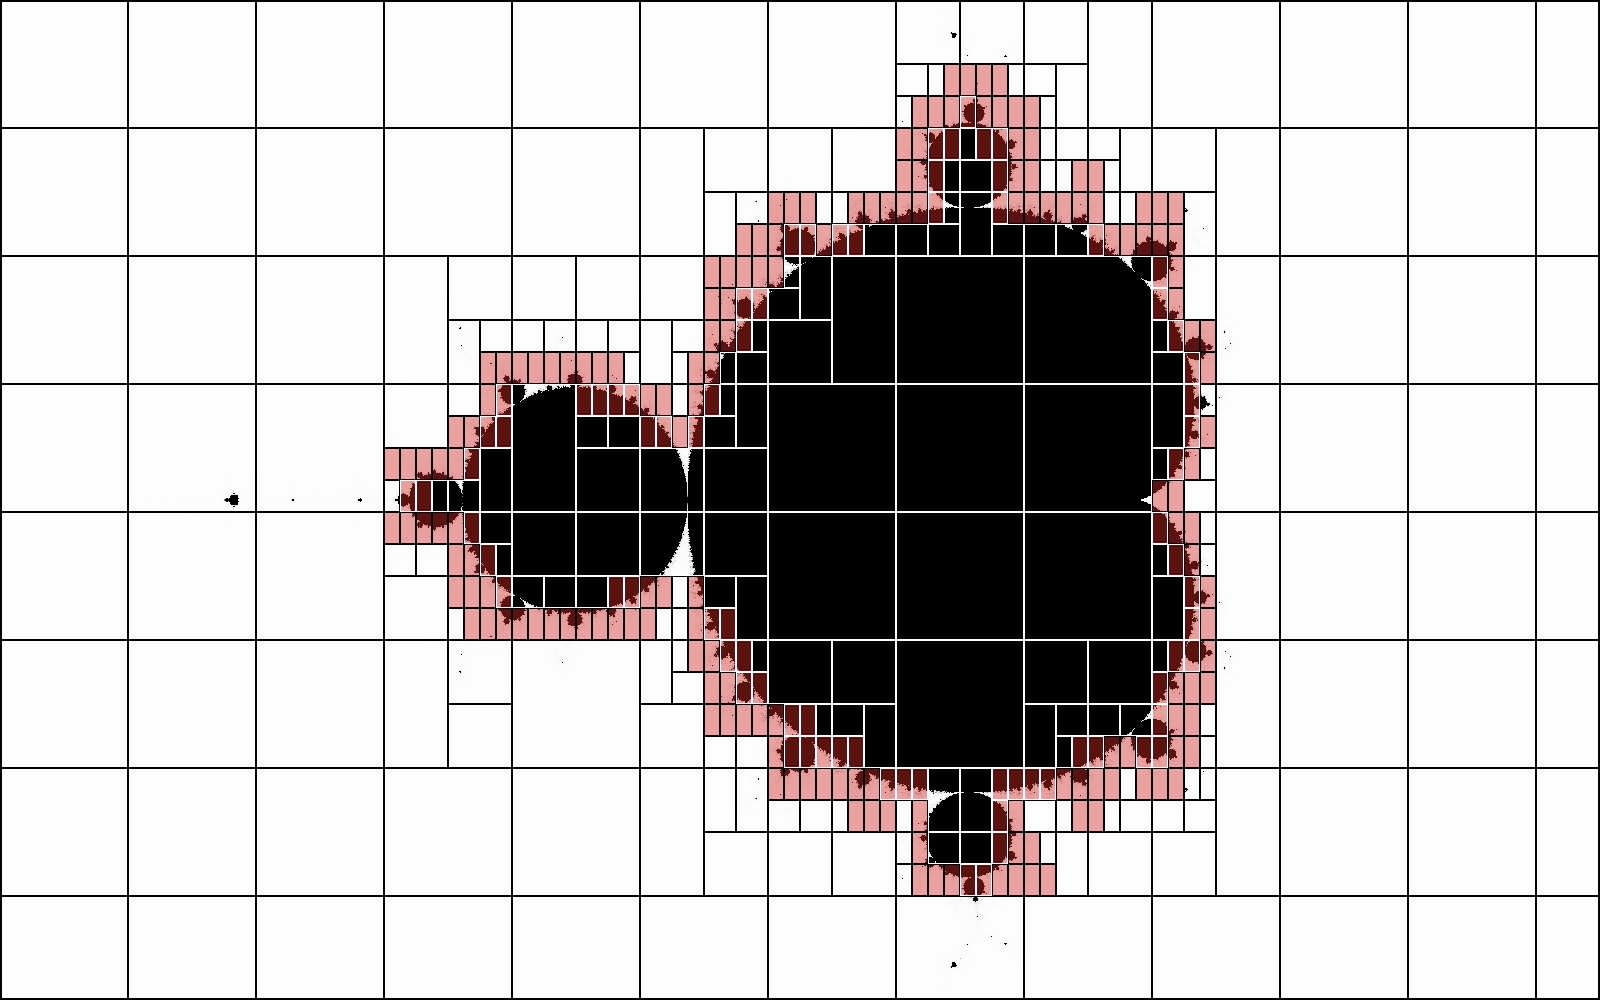
\includegraphics[width=0.8\textwidth]{figures/sched-tiling.png}
  \caption{Подела на плочице класификатора приказана на рендеру целог кадра
  Манделбротовог скупа. Плочице класификоване за графички процесор остављене су
  необојене. Плочице класификоване за процесор осенчене су црвено.}
  \label{fig:sched-tiling}
\end{figure}

Слика~\ref{fig:sched-tiling} чини ту концентрацију видљивом. Плочице процесора
формирају танку траку која прати сам облик границе, а не чврсту масу, а рекурзија иде
најдубље управо тамо где тај облик најмање личи на праву линију. Шпицеви на местима
где се главна кардиоида спаја са пратећим балонима издвајају се као мале групе
плочица минималне величине унутар шире траке. То је исти ефекат који стоји иза удела
процесора од $3\%$ до $14\%$ наведеног изнад. Колико год се фино граница набира на
размерама испод једног пиксела, мрежа плочица је у стању да је разложи само до
резолуције минималне плочице, тако да удео процесора остаје везан за то колико од
видљивог кадра граница пресеца, а не за то колико је та крива заправо сложена.

\section{Расподела посла и синхронизација}
\label{sec:work-distribution}

Листа графичког процесора коју производи класификатор не предаје се графичком
процесору у целости. Завршни део те листе, подразумевано $20\%$, уместо тога се
издваја у посебан резервни базен, а остатак, предате плочице, је оно што се
заиста одмах шаље графичком процесору. И резервни базен и листа за процесор, сада
сопствени ред посла, представљају дељено стање о које се боре нити, из којег свака
радна нит процесора може да узима.

По једна радна нит извршава се по доступном језгру процесора, а свака радна нит ради
у петљи. Прво преузима плочицу из свог сопственог реда за процесор, и тек кад се тај
ред испразни посеже у резервни базен, тако да се резервисани посао графичког
процесора дотиче тек након што се потроши сопствени, додељени удео радне нити. Док те
радне нити раде истовремено, графички процесор се покреће на предатим плочицама у
једном пакету, тако да ниједан уређај не чека другог за већи део кадра. Када се то
покретање заврши, распоређивач проверава колико је плочица још увек непреузето у
резервном базену. Ако их остане бар $64$, радници на процесору очигледно до њих још
нису дошли, још увек заузети сопственим редом, па се исплати још једно покретање
графичког процесора да заврши остатак, уместо да се чека да их процесор на крају
испразни. У супротном, остатак је довољно мали да сопствени трошак другог покретања
графичког процесора не би вредео, па се једноставно оставља радницима на процесору да
га настављају да краду. Читање с графичког процесора које следи копира цео бафер
кадра без обзира на то који је удео графички процесор заиста рендеровао, пошто би
смањивање тог копирања захтевало да удео графичког процесора буде један непрекидан
опсег редова, а не расути скуп плочица.

Када и сваки радник на процесору и покретање графичког процесора заврше, рендероване
плочице сваког уређаја копирају се на своју стварну позицију у дељени излазни бафер.
Током самог рендеровања није потребно ниједно закључавање по пикселу или по плочици,
само кратак тренутак у ком радник преузима плочицу из реда. Плочице које рендерују
графички процесор и радник на процесору увек су дисјунктне, тако да корак спајања
који следи нема ниједан сукоб да разрешава.

\section{Адаптивно балансирање оптерећења помоћу PI регулатора}
\label{sec:load-balancing}

Праг класификатора (одељак~\ref{sec:tile-decomposition}) замена је за то колико
дивергентна ће вероватно бити унутрашњост плочице, а не директно мерење тога који
уређај ту плочицу рендерује брже, а права вредност те замене зависи од садржаја сцене
и од релативног оптерећења два уређаја на начине које ништа пре самог рендеровања не
може унапред знати. Регулатор повратне спреге уместо тога затвара петљу споља. Он
посматра стварно измерено GPU и CPU време сваког кадра и благо помера праг тако да
оба уређаја остану уравнотежена у наредном кадру.

Регулатор прати једну означену грешку по кадру, $\mathrm{error} = t_{\mathrm{gpu}} -
t_{\mathrm{cpu}}$, разлику између измереног времена рендеровања на графичком
процесору и на процесору за тај кадар, и ажурира праг као
\begin{equation}
  \label{eq:pi-controller}
  \mathrm{threshold} \mathrel{-}= K_P \cdot \mathrm{error} + K_I \cdot \overline{\mathrm{error}},
\end{equation}
уз $K_P = 0.0005$ и $K_I = 0.00005$, а затим се резултат ограничава на опсег $[0.001,
0.5]$. Позитивна грешка значи да је графички процесор тог кадра био спорији од
процесора, а једначина~\ref{eq:pi-controller} на то одговара снижавањем прага. Пошто
је сам тест класификатора $\mathrm{spread} < \mathrm{threshold}$, нижи праг је строжи
захтев за униформношћу, па мање плочица пролази тест, а више их се усмерава ка
процесору у наредном кадру, растерећујући уређај који је заостајао. Негативна грешка
помера праг у супротном смеру. Само пропорционални члан реагује искључиво на
тренутни кадар и оставио би устаљену пристрасност некоригованом ако је један уређај
\emph{доследно} бржи, а не само шумно бржи од кадра до кадра. Интегрални члан
$\overline{\mathrm{error}}$, покретни просек преко последњих $16$ кадрова, а не
неограничена текућа сума, исправља ту преосталу пристрасност, а истовремено дозвољава
да утицај једног шумног кадра избледи после шеснаест ажурирања, уместо да траје
заувек. Пропорционално појачање десет је пута веће од интегралног, тако да регулатор
најбрже реагује на кадар који је управо измерен, а на интегрални члан се ослања само
за оно што пропорционални сам не исправи. Ограничење на $[0.001, 0.5]$ спречава да
велика, устаљена неравнотежа, попут застоја драјвера графичког процесора, одвуче праг
у крајност у којој се класификатор своди на усмеравање свега ка једном уређају без
обзира на садржај, чиме би се одбацила управо она свест о садржају коју је
одељак~\ref{sec:tile-decomposition} и изграђен да пружи.

\begin{figure}[H]
  \centering
  
\includegraphics[width=0.75\textwidth]{figures/sr/pi-controller-response.png}
  \caption{Симулација једначине~\ref{eq:pi-controller} кроз $70$ синтетичких кадрова,
  са привременим застојем графичког процесора убаченим између кадрова $25$ и $50$.
  Праг пада док застој траје, усмеравајући већи део кадра ка процесору, а прозор
  интеграла од шеснаест кадрова наставља да га вуче надоле још неколико кадрова након
  што застој престане, пре него што се пропорционални члан поново стабилизује на
  шуму средње вредности нула. Ово извршавање случајно достиже доњу границу од
  $0.001$, илуструјући управо случај за који је горње ограничење и постављено.}
  \label{fig:pi-controller-response}
\end{figure}

Листинг~\ref{lst:pi-controller} је цео регулатор, свега двадесетак линија.
Ажурирање \kod{self.\allowbreak integral} рачуна покретни просек преко \kod{history}, кружног
бафера последњих $16$ грешака, а последње две линије тела \kod{update} су директно
једначина~\ref{eq:pi-controller}, укључујући ограничење опсега.

\noindent\begin{minipage}{\linewidth}
\lstinputlisting[language=Rust, numbers=none,
  caption={PI регулатор прага класификатора
  (\kod{src/scheduler/controller.rs}).},
  label={lst:pi-controller}]{listings/pi_controller.rs}
\end{minipage}

Пошто интерактивно рендеровање изнова рендерује кадар при сваком померању и увећању,
ова повратна спрега ради непрекидно, а не као једнократни корак калибрације.
Ажурирање се извршава на крају сваког хетерогеног рендеровања, а праг који оставља за
собом тачно је оно што класификатор из одељка~\ref{sec:tile-decomposition} чита на
почетку самог следећег. Заједно са крађом унутар кадра из
одељка~\ref{sec:work-distribution}, распоређивач исправља неравнотежу оптерећења на
две временске скале истовремено. Крађа апсорбује графички процесор који заостаје
унутар једног кадра, а регулатор апсорбује графички процесор који заостаје
\emph{кроз} кадрове, преобликујући саму класификацију. Глава~\ref{ch:results} мери
колико од трошка читања с којим је ова глава почела та комбинација заиста надокнади,
и где су два уређаја довољно блиска по брзини да исправка уопште буде важна.

\chapter{Експериментална методологија}
\label{ch:methodology}

Глава~\ref{ch:results} извештава о времену кадра, пропусности и понашању при
скалирању за свако позадинско решење изграђено у главама~\ref{ch:algorithms},
\ref{ch:gpu} и~\ref{ch:scheduler}. Ова глава дефинише услове под којима су те бројке
добијене. Одељак~\ref{sec:technology-stack} обрађује софтверски стек и начин на који
је конфигурисан и мерен. Одељак~\ref{sec:hardware} обрађује машину.
Одељак~\ref{sec:benchmarks} обрађује коришћене фрактале, резолуције и приказе, а
одељак~\ref{sec:metrics} обрађује извештаване величине.

\section{Технолошки стек}
\label{sec:technology-stack}

\subsection{Rust}
\label{sec:rust}

Rust је компајлирани системски језик без сакупљача отпадака (енг. \emph{garbage
collector}). Безбедност меморије и одсуство трка над подацима спроводе се у време
компајлирања, кроз проверу власништва и позајмљивања, а не путем сакупљача који ради
у реалном времену. Та гаранција је важна за рендерер чија је извештавана јединица
време кадра у милисекундама. Имплементација са сакупљачем отпадака захтевала би да се
свако мерење раздвоји на паузе сакупљања и алгоритамски трошак пре него што иједна
бројка у глави~\ref{ch:results} нешто значи, а овај рендерер нема такво раздвајање да
прави. Компајлер своди код на нативни машински код кроз LLVM, тако да се генерички и
итераторски заснован Rust код компајлира у исти машински код као и еквивалентна ручно
написана петља. Блокови \kod{unsafe}, коришћени само за позиве CUDA драјвера, једини
су излаз из провера компајлера.

Пројекат циља издање 2024 и гради се кроз две конфигурације у време компајлирања,
примењене уједначено на сваку бројку у овом раду.
\begin{itemize}
  \item release профил, \kod{opt-level = 3}, \kod{lto = "thin"}, „танка''
  оптимизација у време линковања кроз читав граф зависности, и
  \kod{codegen-units = 1}, једна јединица генерисања кода, чиме се време
  компајлирања жртвује за потпуну видљивост оптимизатора у програм. Ниједно мерење у
  овом раду не потиче из debug верзије, која је за читав ред величине спорија и није
  употребљива основа за поређење, и
  \item \kod{-C target-cpu=native}, постављено преко \kod{rustflags}, што компајлеру
  дозвољава да циља сваки скуп инструкција који процесор референтне машине
  (одељак~\ref{sec:hardware}) заиста поседује, укључујући AVX2 инструкције у које се
  компајлирају SIMD кернели \kod{f32x8}/\kod{f64x4}. Конзервативан подразумевани циљ
  уопште не би генерисао те инструкције.
\end{itemize}

Четири крејта носе имплементацију на страни процесора. Овде се наводи за шта се сваки
од њих користи, а не како, пошто одељак~\ref{sec:baseline-scalar} и
одељак~\ref{sec:simd} већ обрађују саме кернеле.
\begin{itemize}
  \item \kod{rayon}, базен нити са крађом посла (енг. \emph{work stealing}) иза сваког
  кернела на процесору, скаларног и SIMD подједнако,
  \item \kod{wide}, преносиви SIMD векторски типови \kod{f64x4}/\kod{f32x8},
  \item \kod{num-complex}, аритметика комплексних бројева коју итерирају кернели
  алгоритма бекства, и
  \item \kod{image}, за упис рендерованих кадрова у PNG ради провере излаза.
\end{itemize}

\subsection{GPU технологије}
\label{sec:gpu-tech}

Две технологије графичког процесора стоје иза два GPU кернела упоређена у овом раду, а
разликују се по томе шта овом раду дозвољавају да контролише у време компајлирања.
WebGPU је преносив API за израчунавање и графику, стандардизован независно од било
ког појединачног произвођача. Драјвер га пресликава на било који нативни API који
платформа изложи, на референтној машини Vulkan. Његови шејдери су написани у WGSL-у и
компајлирани у реалном времену од стране драјвера, тако да један изворни код кернела
ради непромењен на сваком уређају способном за WebGPU, по цени изостанка контроле у
време компајлирања над машинским кодом који на крају производи сопствени компајлер
драјвера. Овај рад приступа WebGPU-у преко \kod{wgpu} (верзија~22), Rust
имплементације коју такође користе Firefox и Deno.

CUDA је затворена платформа компаније NVIDIA за израчунавање. Кернели се унапред
компајлирају помоћу \kod{nvcc} у PTX, NVIDIA-ину стабилну посредну репрезентацију,
уграђену у компајлирани извршни фајл, тако да ништа не мора да се компајлира у
реалном времену. Пет заставица конфигурише то компајлирање, примењених идентично на
сваки CUDA кернел у овом раду.
\begin{itemize}
  \item \kod{--gpu-architecture=sm\_86}, директно циљајући генерацију Ampere
  референтног графичког процесора (одељак~\ref{sec:hardware}), уместо генеричког
  циља који би драјвер морао да преводи при учитавању,
  \item \kod{-O3}, највиши ниво оптимизације алата \kod{nvcc},
  \item \kod{--ftz=false}, чиме се задржавају денормализовани бројеви покретног
  зареза, потребни за тачност формуле глатког бојења близу прага бекства,
  \item \kod{--prec-div=true}, дељење пуне прецизности, и
  \item \kod{--fmad=false}, чиме се искључује сажимање спојеног множења и сабирања,
  тако да CUDA-ина аритметика заокружује потпуно исто као и кернели на процесору, уз
  измерени трошак испод $1\%$ пропусности кернела када се уклоне остали трошкови
  прецизности (одељак~\ref{sec:cuda}).
\end{itemize}
Овај рад приступа CUDA~12 преко \kod{cudarc}, Rust везивног слоја (енг. \emph{binding}) за
API CUDA драјвера.

\subsection{Технологија бенчмаркинга}
\label{sec:benchmarking-tech}

Три алата мере рендерер, сваки прилагођен другачијој намени.
\begin{itemize}
  \item \kod{criterion}, статистички крејт за бенчмаркинг, извршава главни пакет
  (\kod{fractal\_\allowbreak bench}). Свака група добија двосекундно загревање, које се
  одбацује, а затим пет секунди мерења, и извештава средњу вредност са интервалом
  поверења од $95\%$, а не једним узорком. Поновљена извршавања номинално
  идентичног кернела разликовала су се за више од $50\%$ унутар једног позива алата
  \kod{criterion}.
  \item \kod{bench\_\allowbreak runner}, наменски израђен извршни фајл који детерминистички
  рендерује једну фиксну конфигурацију, за упаривање са \kod{perf stat} или за
  издавање машински читљивог JSON-а, и
  \item скуп самосталних извршних фајлова-сонди (\kod{gpu\_probe},
  \kod{ptx\_variants}, \kod{sched\_probe}, \kod{sched\_\allowbreak overhead},
  \kod{sched\_\allowbreak deepzoom}, \kod{tiled\_dispatch\_\allowbreak probe}, \kod{adapters}), од којих сваки
  изолује једну фазу или једну хипотезу коју једна бројка времена кадра сама по себи
  не може раздвојити: на пример време кернела од времена читања на страни хоста,
  ефекат једне компајлерске заставице од ефекта друге, или трошак распоређивача од
  квалитета његових одлука.
\end{itemize}
\kod{perf stat} обезбеђује бројаче кеша и грана на процесору, NVIDIA Nsight Compute
обезбеђује бројаче заузетости и ефикасности „warp''-ова на графичком процесору, а
RAPL (енг. \emph{Running Average Power Limit}) бројачи потрошње енергије пакета, заједно са потрошњом снаге коју извештава
\kod{nvidia-smi}, обезбеђују бројке о енергији у одељку~\ref{sec:scaling-energy}.

Четири постојећа рендерера прегледана у одељку~\ref{sec:related-work} не деле ништа
од овог алата. Сваки је за потребе овог рада опремљен еквивалентним двослојним
оквиром за мерење, циљем \kod{criterion\_bench} заснованим на Google Benchmark-у и
CLI позивом \kod{bench\_runner} који директно позива сопствени компајлирани кернел
тог пројекта, тако да свих пет рендерера ради из једне командне линије и производи
упоредив JSON. Сопствени модел рада са нитима сваког рендерера мери се онакав какав је
изграђен, а не нормализован на базен алата \kod{rayon}. Поређење циља алгоритамску
пропусност по стварно израчунатом пикселу, па се свака пречица коју пројекат користи
да избегне директно израчунавање пиксела, попут XaoS-овог праћења границе
(енг. \emph{boundary tracing}) или FractalNow-ове интерполације по четворкама
(енг. \emph{quad interpolation}), искључује. Обе замењују израчунавање интерполацијом на
делу слике, што би мерило колико добро пројекат нагађа, а не колико брзо ради његов
кернел.

\section{Хардвер}
\label{sec:hardware}

Сва мерења у овом раду, кроз рад називана референтном машином, потичу са једног
лаптопа, изграђеног око следећег.
\begin{itemize}
  \item процесора AMD Ryzen~7 5800H, осам језгара Zen~3, шеснаест нити преко
  двоструког SMT-а,
  \item графичког процесора NVIDIA GeForce RTX 3050 Laptop GPU, Ampere (\kod{sm\_86}),
  CUDA 12.0, драјвер 580.173.02, PCIe~3.0 x8 (теоријски $8\,\mathrm{GB/s}$), и
  \item интегрисаног графичког процесора AMD Radeon Vega, кодног имена Renoir.
\end{itemize}

Слика~\ref{fig:hardware-topology} приказује како су ове компоненте заправо повезане.
Чип Ryzen носи интегрисани графички процесор Radeon Vega на истом паковању, тако да
оба деле исту двоканалну DDR4 системску RAM меморију преко једног контролера меморије
на чипу, потпуно без PCIe преноса између њих. RTX 3050 је посебан, дискретан део,
доступан само преко PCIe~3.0 x8, са сопственом наменском GDDR6 VRAM меморијом коју
процесор не може директно да адресира, управо она веза чији трошак
одељак~\ref{sec:gpu-traversal} и глава~\ref{ch:scheduler} у великој мери настоје да
заобиђу у овом раду.

\begin{figure}[H]
  \centering
  \begin{tikzpicture}[
    font=\small,
    comp/.style={rectangle, rounded corners, draw=black, thick, minimum width=3.6cm,
      minimum height=1.1cm, align=center, inner sep=4pt, fill=blue!10},
    gpucomp/.style={comp, fill=green!12},
    memcomp/.style={comp, fill=gray!12},
    pkg/.style={rectangle, rounded corners, draw=black, thick, dashed, inner sep=10pt},
    arrow/.style={{Stealth[length=2.2mm]}-{Stealth[length=2.2mm]}, thick},
  ]
  \node[comp]     (cpu)  at (0,0)   {AMD Ryzen~7 5800H\\8 језгара / 16 нити};
  \node[gpucomp]  (igpu) at (0,-1.7) {AMD Radeon Vega (Renoir)\\интегрисани GPU};

  \node[pkg, fit=(cpu)(igpu), label={[font=\scriptsize]above:паковање процесора (један чип)}] (pkgbox) {};

  \node[memcomp]  (ram)  at (-6.2,-0.85) {системска RAM\\двоканална DDR4};

  \node[gpucomp]  (dgpu) at (6.4,-0.85) {NVIDIA GeForce RTX 3050\\Laptop GPU (дискретни)};
  \node[memcomp, minimum width=3cm]  (vram) at (6.4,-2.7) {наменска GDDR6 VRAM};

  \draw[arrow] (ram) -- (pkgbox.west|-ram)
    node[midway, above, font=\tiny, align=center] {контролер меморије\\на чипу};
  \draw[arrow] (pkgbox.east|-dgpu) -- (dgpu)
    node[midway, above, font=\tiny, align=center] {PCIe 3.0 x8\\$\sim$7.9 GB/s};
  \draw[arrow] (dgpu) -- (vram)
    node[midway, right, font=\tiny, align=left] {магистрала меморије\\на плочи};
  \end{tikzpicture}
  \caption{Топологија компоненти референтне машине. Интегрисани графички процесор
  дели паковање процесора и системску RAM меморију без икаквог трошка преноса.
  Дискретни графички процесор доступан је само преко PCIe магистрале, са сопственом
  одвојеном VRAM меморијом.}
  \label{fig:hardware-topology}
\end{figure}

Избор адаптера алата \kod{wgpu} тихо се враћа на интегрисани графички процесор када
није инсталиран NVIDIA Vulkan драјвер, чиме потцењује трошак читања с графичког
процесора, пошто интегрисани део дели меморију са процесором и уопште не плаћа PCIe
пренос. Свака сесија бенчмарка бележи изабрани адаптер при покретању, што се
проверава пре него што се његове бројке употребе.

Референтна машина је лаптоп, а не наменска машина за бенчмарк, и термички је
промењива. Идентични бенчмаркови процесора или графичког процесора, покренути у
одвојеним сесијама без икакве промене кода између њих, помакли су се за $15$ до
$30\%$ само услед термичког стања. Свака размера и бројка убрзања у
глави~\ref{ch:results} рачуна се унутар једног извршавања. Апсолутне бројке у
милисекундама ипак носе ту варијансу.

\section{Бенчмаркови и тест сцене}
\label{sec:benchmarks}

\subsection{Фрактали, резолуције и бројеви итерација}
\label{sec:bench-resolutions}

Манделбротов скуп је једини циљ бенчмарка у овом раду. Рендерер такође имплементира
Жулијине, Њутнове и Нова фрактале на истој машинерији алгоритма бекства, али је свака
оптимизација у главама од~\ref{ch:algorithms} до~\ref{ch:scheduler}, тестови
кардиоиде и балона, процена растојања, Мариани-Силвер подела, као и рад на SIMD и
GPU кернелима, развијена и мерена конкретно на Манделбротовом скупу, и управо о
томе извештава остатак овог рада.

Пакет бенчмаркова тестира Манделбротов скуп на три резолуције, $800\times600$,
$1920\times1080$ и $3840\times2160$, изабране да потврде да добит технике важи
независно од величине кадра. Осим ако сама серија мерења не каже другачије,
\kod{max\_iter} је фиксирано на $1000$. Један изузетак је провера конвергенције у
односу на површину Манделбротовог скупа, у литератури процењену на приближно
$1.50659177$, која варира сам \kod{max\_iter}, од $100$ до $20000$.

\subsection{Прикази}
\label{sec:bench-viewports}

Већина бенчмаркова рендерује цео видљиви скуп из његовог природног центра
($c=-0.5$, увећање $1$), мешајући унутрашње, граничне и брзо-бежеће пикселе
приближно у пропорцијама какве показује интерактивна сесија. Тамо где трошак технике
конкретно зависи од тога колико кадра чини граница, а не унутрашњост, пакет уместо
тога користи пет фиксних узорачких тачака које обухватају главну кардиоиду, највећи
балон, мини-Манделброт и област густу нитима, како резултат не би могао бити
артефакт једног погодног приказа са мало границе у њему.

\begin{figure}[H]
  \centering
  
\includegraphics[width=0.75\textwidth]{figures/sr/benchmark-viewport-map.png}
  \caption{Пет фиксних узорачких тачака, изабраних да обухвате приказ целог скупа,
  граничну област густу нитима, мини-Манделброт и каскаду удвостручавања периода ка
  Фајгенбаумовој тачки дуж негативне реалне осе. Тачка „долине морских коњица''
  истовремено служи и као референтни центар за серије увећања у
  одељку~\ref{sec:bench-zoom-sweeps}.}
  \label{fig:benchmark-viewport-map}
\end{figure}

\subsection{Серије увећања}
\label{sec:bench-zoom-sweeps}

Три серије мерења испитују понашање зависно од увећања. Плитка серија (увећање $1$,
$10^2$, $10^4$) остаје испод прага $10^6$ на ком и кернели за процесор и они за
графички процесор прелазе са \kod{f32} на \kod{f64}. Дубока серија (увећање од
$10^4$ до $10^{15}$) прелази тај праг, на фиксној референтној тачки „долине морских
коњица'' ($c=-0.75+0.1i$), изабраној зато што њена граница остаје довољно густа, на
сваком нивоу увећања у серији, да класификатору плочица пружи стваран посао. Трећа
серија (увећање од $1$ до $10^{12}$, иста референтна тачка) вреднује теорију
пертурбације у односу на обичан \kod{f64}.

\subsection{Поређење између рендерера}
\label{sec:bench-cross-renderer}

Поређење са четири постојећа рендерера ограничено је на оно што свих пет пројеката
дели, кернел за Манделбротов скуп, при усклађеној резолуцији, броју итерација и
приказу, мерено као сирово време итерације по пикселу, а не као потпуно обојени
кадрови, пошто се рендерери разликују по томе колико посла мапирања боје је стопљено
у тај корак.

\section{Метрике}
\label{sec:metrics}

\subsection{Време кадра и пропусност}
\label{sec:metrics-throughput}

Време кадра извештава се као средња вредност узорка алата \kod{criterion}, са
његовим интервалом поверења. Пропусност, број рендерованих пиксела по милисекунди,
добија се из истог мерења преко механизма бројања елемената алата \kod{criterion}, а
не изводи накнадно. Равна крива пропусности кроз резолуције представља радну
дефиницију „сасвим паралелног'' (енг. \emph{embarrassingly parallel}) кернела у овом раду.
Крива која се савија указује на трошак који расте са величином кадра, а не само са
бројем пиксела.

\subsection{Ефикасност израчунавања}
\label{sec:metrics-gflops}

Поређења између кернела додатно се исказују у GFLOPS-има, по једној фиксној
конвенцији. Свака итерација канонског ажурирања $z = z^2 + c$ рачуна се као осам
операција покретног зареза, без урачунавања сажимања спојеног множења и сабирања.
Конвенција је поједностављење, а не дословно бројање инструкција, али управо њена
уједначена примена, и на сопствене кернеле овог рендерера и на сва четири
конкурентска пројекта, чини бројку у GFLOPS-има упоредивом између пет независно
написаних кодних база.

\subsection{Поређење контролисано по прецизности}
\label{sec:metrics-precision}

Свако извештено убрзање наводи прецизност, \kod{f32} или \kod{f64}, при којој су
обе стране радиле. Упаривање брзог \kod{f32} кернела на графичком процесору са спором
\kod{f64} основном варијантом на процесору вештачки увећава привидни добитак,
независно од стварне пропусности било ког уређаја, ефекат који Ли и др. документују
за поређења процесора и графичког процесора уопште \cite{lee2010debunking}. Сваки
однос графичког процесора и процесора у овом раду наводи се најмање двапут: једном
у односу на наивну скаларну основну варијанту, а једном у односу на најбољи доступан
сопствени кернел процесора при подударајућој прецизности.

\subsection{Паралелно скалирање и енергија}
\label{sec:scaling-energy}

Скалирање по нитима извештава се као убрзање и паралелна ефикасност у односу на
сопствено једнонитно извршавање истог рендерера, никада између различитих рендерера,
пошто се модели нитовања структурно разликују између пројеката. Енергетска
ефикасност извештава се одвојено од брзине, као гигафлопси по вату, из RAPL бројача
потрошње енергије пакета (за процесор) и потрошње снаге коју извештава
\kod{nvidia-smi} (за графички процесор) током дужег извршавања, пошто спорији уређај
није нужно и мање ефикасан.

\subsection{Тачност и микроархитектонске метрике}
\label{sec:correctness-metrics}

Две додатне метрике примењују се тамо где питање није о брзини. Где оптимизација
треба да мења само перформансе, а не излаз, тачност се проверава бројањем разлика по
пикселу између варијанти кернела; нула разлика кроз цео кадар је услов пре објаве
бројке брзине. Где хипотеза тиче понашања на графичком процесору, на пример
дивергенције „warp''-ова у граничним областима, то разрешавају заузетост и
ефикасност „warp''-ова из Nsight Compute, независно од утицаја на време кадра.

\chapter{Резултати и дискусија}
\label{ch:results}

Ова глава представља мерења која поставка из главе~\ref{ch:methodology} производи.
Свака слика потиче са ту дефинисане референтне машине, а сваки овде наведени однос
прати правила поређења контролисаног по прецизности и унутар истог извршавања,
изложена у одељку~\ref{sec:metrics}. Већина слика у овој глави генерисана је директно
алатом \kod{aggregate\_\allowbreak bench.py} овог пројекта, описаним у
одељку~\ref{sec:technology-stack}, из једног архивираног извршавања бенчмарка, а не
поново нацртана ручно, тако да бројка која изгледа мало другачије од оне већ наведене
у ранијој глави представља термичку варијансу између извршавања, врсту коју описује
одељак~\ref{sec:hardware}, а не противречност. Глава прати редослед којим су главе од
~\ref{ch:algorithms} до~\ref{ch:scheduler} увеле основне технике: прво основну
варијанту на процесору и SIMD, затим два позадинска решења за графички процесор, цео
цевовод од почетка до краја, хибридни распоређивач, теорију пертурбације и на крају
резултате поређења између пројеката и нумеричке валидације. Два резултата носе више
тежине од осталих. Слика~\ref{fig:results-gpu-resolution} у одељку~\ref{sec:results-gpu}
јединствено је мерење у које се улива свака ранија глава оптимизације, пропусност
рендеровања за свако позадинско решење изграђено у овом раду, једно поред другог, а
одељак~\ref{sec:results-scheduler} је место где се хибридни распоређивач, централни
допринос овог рада, проверава наспрам алтернативе простог избора бржег уређаја и
наспрам поделе коју би теоријски требало да може да достигне.

\section{Основна варијанта на процесору и SIMD скалирање}
\label{sec:results-cpu}

Слика~\ref{fig:results-thread-scaling} потврђује скалирање по нитима које описује
одељак~\ref{sec:baseline-scalar}. ruster-ово паралелно блоковање редова помоћу
\kod{rayon}-а остаје близу праве линије на графику логаритамске размере кроз осам
нити, и тек код шеснаест се савија, потпис симултаног вишенитног извршавања (SMT), где
друга логичка нит на већ заузетом физичком језгру купује само део пуног језгра, а не
још једно удвостручавање. FractalRendererCpp скалира лошије при сваком броју нити,
делом зато што покреће и придружује свеж \kod{std::thread} по кадру, уместо да поново
користи базен, трошак имплементације наведен у одељку~\ref{sec:bench-cross-renderer},
који ово поређење укључује у бројку по нити, уместо да га издваја.

\begin{figure}[H]
  \centering
  
\includegraphics[width=0.7\textwidth]{figures/sr/ruster-thread-scaling.png}
  \caption{Скалирање по нитима на процесору, ruster наспрам FractalRendererCpp,
  Манделбротов скуп, 1080p, скаларни \kod{f64} на обе стране.}
  \label{fig:results-thread-scaling}
\end{figure}

Слика~\ref{fig:results-simd-progression} приказује напредак SIMD кернела из
одељка~\ref{sec:simd}, мерен на 1080p и 4K. Сваки корак, \kod{f64x4}, \kod{f32x8}, а
затим кернел са два ланца \kod{f32x8+ILP}, снижава време кадра, а образац се готово
идентично понавља на обе резолуције, доказ да је добитак својство кернела, а не
одређене величине кадра. Убрзање од скаларне варијанте до \kod{f32x8+ILP} износи
$1.92\times$ на 1080p и $2.37\times$ на 4K, при чему корак паралелизма на нивоу
инструкција доприноси мање од десетине тога. Одељак~\ref{sec:simd} мали остатак
приписује томе што тестови кардиоиде и балона већ уклањају већину пиксела који би
иначе попунили цевовод другог ланца.

\begin{figure}[H]
  \centering
  
\includegraphics[width=0.75\textwidth]{figures/sr/results-simd-progression.png}
  \caption{Напредак SIMD кернела на процесору, Манделбротов скуп, 1080p и 4K.}
  \label{fig:results-simd-progression}
\end{figure}

Слика~\ref{fig:results-cpu-microopt} проверава још два избора на страни процесора
наспрам обичне основне варијанте са блоковањем редова у \kod{rayon}-у. Леви панел је
питање редоследа обиласка из одељка~\ref{sec:traversal-locality}, Хилбертов
обилазак наспрам обичног по редовима, а измерена разлика директно
потврђује тврдњу тог одељка. Хилбертов обилазак рендерује спорије на свакој
испитаној резолуцији, отприлике $224$ наспрам $133$ Mpix/s при $800\times600$, а
разлика се сужава, али се не затвара до $3840\times2160$, без икаквог компензујућег
добитка локалности кеша за додатни трошак преплитања битова по пикселу. Десни панел је
питање паралелизма на нивоу инструкција из одељка~\ref{sec:simd} посматрано само за
себе, преплетени кернел \kod{f32x8+ILP} наспрам обичног \kod{f32x8}, и преплетени
кернел је бољи на свакој испитаној резолуцији, од уске разлике од $3\%$ при
$800\times600$ до отприлике $9\%$ на $1080$p, у складу са добитком који захтева
довољно независног посла по пикселу у лету да би се исплатило књиговодство другог
ланца.

\begin{figure}[H]
  \centering
  
\includegraphics[width=\textwidth]{figures/sr/ruster-cpu-microopt.png}
  \caption{Микрооптимизације на процесору, Хилбертов наспрам обиласка по редовима и
  обичан наспрам преплетеног \kod{f32x8}, Манделбротов скуп.}
  \label{fig:results-cpu-microopt}
\end{figure}

\FloatBarrier

\section{Позадинска решења за графички процесор}
\label{sec:results-gpu}

Слика~\ref{fig:results-gpu-resolution}, прва у овом одељку, средишња је тачка ове главе.
Свака измерена оптимизација постоји да би померила једну бројку: колико пиксела
позадинско решење рендерује у секунди. Она ставља свако позадинско решење
изграђено у овом раду на исте осе: скаларни CPU, SIMD CPU, CUDA, wgpu, и сва
четири конкурентска пројекта из одељка~\ref{sec:bench-cross-renderer}, Fractals-rs,
FractalRendererCpp, XaoS и FractalNow, на три резолуције, тако да је цео напредак од
процесора до графичког процесора видљив на једном месту, уместо расутог по читавој
глави одвојених панела. XaoS и FractalNow мерени су на свом сировом кернелу по
пикселу, са принудно искљученим праћењем границе и интерполацијом по четворкама, како
одељак~\ref{sec:bench-cross-renderer} објашњава, а не на мерењу стварног
интерактивног мотора било ког пројекта. Друга, шрафирана трака за XaoS поново укључује
праћење границе: $50.8$, $85.3$ и $114.4$ Mpix/s кроз три резолуције, $21\times$ до
$36\times$ у односу на сопствени сирови кернел, и већ испред сопствене вишенитне траке
сировог кернела, упркос томе што ради на једној нити, пошто је путања која ради са нитима у
\kod{btrace.cpp} искључена узводно. То је један статички кадар без претходног кадра
из кога би се нагађало, тако да мери само алгоритам праћења границе и попуне
(енг. \emph{flood fill}), а не додатно поновно коришћење између кадрова које доноси
стварни аниматор увећања у XaoS-у, и није упоредив ни са једном другом, вишенитном
траком на овој слици.

CUDA предњачи над сваким другим позадинским решењем на свакој резолуцији, wgpu је
други, а разлика између два GPU позадинска решења остаје приближно сразмерна
величини кадра, у складу са фиксним трошком кернела по пикселу, а не фиксним трошком
по кадру који би доминирао било којим од њих. Врхунска пропусност, при
$3840\times2160$, достиже отприлике $1389$ Mpix/s на CUDA-и. Две црвене траке
хибридног распоређивача постоје само на $1080$p, пошто та група бенчмаркова варира
увећање при једној фиксној резолуцији, а не резолуцију при једном фиксном увећању, а
одељак~\ref{sec:results-scheduler} их чита директно, а не преко ове слике.

\begin{figure}[H]
  \centering
  
\includegraphics[width=\textwidth]{figures/sr/ruster-throughput-all-backends.png}
  \caption{Пропусност рендеровања, свако позадинско решење ruster-а и сва четири
  конкурентска пројекта, Fractals-rs, FractalRendererCpp, XaoS, FractalNow, три
  резолуције, Манделбротов скуп, увећање 1. Кључно мерење ове главе. Свака CPU и GPU
  оптимизација од главе~\ref{ch:algorithms} до главе~\ref{ch:gpu} овде се очитава као
  растојање између једне и следеће траке. Шрафирана трака за XaoS представља његов
  стваран алгоритам „нагађања'' праћењем границе, једна нит, један статички кадар,
  неупоредив са вишенитним тракама око ње.}
  \label{fig:results-gpu-resolution}
\end{figure}

Читане слева удесно унутар било које групе резолуција, траке прате цео пут
оптимизације овог рада. Од скаларног до SIMD-а је рад главе~\ref{ch:algorithms}, од
SIMD-а до било ког GPU позадинског решења је рад главе~\ref{ch:gpu}. Предност CUDA-е
над SIMD-ом на процесору, отприлике $2.5\times$ до $3.4\times$ у зависности од
резолуције, повраћај је улагања у изградњу GPU позадинског решења уопште, а остатак
овог одељка објашњава где унутар те CUDA бројке заправо одлази време.

Слика~\ref{fig:results-gpu-breakdown} издваја зашто CUDA побеђује у кадру. Два
кернела разликују се за мање од $5\%$, али читање на страни хоста чини $83\%$ CUDA
кадра и $88\%$ wgpu кадра, а wgpu на то троши отприлике $0.8\,\mathrm{ms}$ више, у
складу са додатним међукопирањем са уређаја на уређај које CUDA-ин једини позив
\kod{dtoh\_sync\_copy} избегава, како одељак~\ref{sec:cuda} објашњава.

\begin{figure}[H]
  \centering
  
\includegraphics[width=0.7\textwidth]{figures/sr/results-gpu-frame-breakdown.png}
  \caption{Расподела времена кадра на графичком процесору, кернел наспрам читања на
  страни хоста, CUDA наспрам wgpu, $1920\times1080$, увећање 1.}
  \label{fig:results-gpu-breakdown}
\end{figure}

Другим речима, оба GPU позадинска решења већи део кадра троше на враћање пиксела
назад ка хосту, а не на њихово рачунање. То преформулише питање
одељка~\ref{sec:results-pipeline} пре него што је уопште постављено. Ако је GPU
позадинско решење већ доминирано преносом података, а не итерацијом, додавање корака
\kod{colorize()} на страни процесора преко тога може ту неравнотежу само учинити
видљивијом, не мањом, осим ако и тај корак не пређе на графички процесор, што је, за
CUDA, и учињено, како описује одељак~\ref{sec:gpu-traversal}.

\FloatBarrier

\section{Цевовод од почетка до краја}
\label{sec:results-pipeline}

Слика~\ref{fig:results-pipeline} додаје корак \kod{colorize()}, мерен пре него што је
било које GPU позадинско решење могло да га прескочи, извршен на процесору подједнако
за свако позадинско решење. Предност графичког процесора над процесором нагло се
сужава када се укључи тај фиксни корак од $2.72\,\mathrm{ms}$, са отприлике $5.4\times$
само на кораку рендеровања на $2.09\times$ за CUDA и $1.72\times$ за wgpu, од почетка
до краја. Од CUDA цевовода од $5.19\,\mathrm{ms}$, отприлике $0.4\,\mathrm{ms}$ отпада
на итерацију фрактала, а преосталих $4.8\,\mathrm{ms}$ на пренос података и бојење.
Управо је то оно што је премештање \kod{colorize()} на графички процесор учинило
једином оптимизацијом са највећим утицајем на коју је ово мерење указало, већом од
исправке fp64 балона из одељка~\ref{sec:cuda} и већом од свега што распоређивач из
главе~\ref{ch:scheduler} може да надокнади. CUDA-ин \kod{colorize()} у међувремену је
премештен на уређај кроз \kod{colorize\_kernel} и \kod{render\_and\_colorize},
описане у одељку~\ref{sec:gpu-traversal}, тачан до пиксела у односу на верзију за
процесор и $54\%$ до $63\%$ бржи од почетка до краја при плитким и средњим увећањима,
тамо где је бојење раније доминирало временом кадра. wgpu и хетерогени распоређивач и
даље боје на процесору. Распоређивач то ради нужно, пошто његов спојени бафер постоји
само на страни хоста, како објашњава глава~\ref{ch:scheduler}, тако да горе описани
добитак остаје отворен за та два пута.

\begin{figure}[H]
  \centering
  
\includegraphics[width=0.65\textwidth]{figures/sr/results-pipeline-end-to-end.png}
  \caption{Време цевовода од почетка до краја, рендеровање плус бојење,
  $1920\times1080$, увећање 1. Мерено са бојењем извршеним на процесору за свако
  позадинско решење, пре него што је CUDA-ин сопствени корак бојења премештен на
  уређај, види текст.}
  \label{fig:results-pipeline}
\end{figure}

Слика~\ref{fig:results-colorize-overhead} раставља исти корак по позадинском решењу,
само рендеровање наспрам рендеровања плус бојење, из истог мерења у ком је свако
позадинско решење бојило на процесору. Фиксни трошак \kod{colorize()} однео је
сразмерно већи залогај код GPU позадинског решења него код процесора, пошто је сваки
пут реч о истом кораку на страни процесора, отприлике петину сопствене пропусности
процесора, али ближе две трећине било ког GPU позадинског решења, исти Амдалов
ефекат који слика~\ref{fig:results-pipeline} већ показује исказан као апсолутно
време, а не као пропорција. Управо је то ефекат који је премештање бојења на графички
процесор учинио вредним за CUDA-у.

\begin{figure}[H]
  \centering
  
\includegraphics[width=0.6\textwidth]{figures/sr/ruster-colorize-overhead.png}
  \caption{Трошак бојења по позадинском решењу, само рендеровање наспрам рендеровања
  плус бојење, Манделбротов скуп.}
  \label{fig:results-colorize-overhead}
\end{figure}

Распоређивач из главе~\ref{ch:scheduler} постоји управо да би повратио оно време које
је овај одељак управо приказао кроз две слике, па се овом главом даље бави управо то.

\FloatBarrier

\section{Хибридни CPU+GPU распоређивач}
\label{sec:results-scheduler}

Овде се централна тврдња овог рада проверава наспрам података. Глава~\ref{ch:scheduler}
изградила је распоређивач који у реалном времену прати оба уређаја и усмерава плочице
према измереном трошку, уместо да слепо дели кадар. Две слике овде су доказ да ли се
та машинерија исплати: на плитком увећању, где би требало да се мучи, и на дубокој
серији увећања, где је осмишљена да побеђује.

Слика~\ref{fig:results-sched-shallow} мери распоређивач из главе~\ref{ch:scheduler}
наспрам оба самостална позадинска решења и наивне статичке поделе, при увећању 1.
Статичка подела $50/50$ процесор плус wgpu, без икакве класификације, најгора је
активна конфигурација на графику, $408$ наспрам wgpu-овог сопственог самосталног
$879$ Mpix/s. То је управо неуспех којим одељак~\ref{sec:work-distribution} мотивише
класификатор узорковањем темена: равна подела оставља бржи уређај да чека спорији.
Адаптивни распоређивач надокнади већи део тог губитка, $688$ Mpix/s на CUDA-и и $549$
на wgpu-у, али и даље заостаје за коришћењем било ког графичког процесора самог.
Свака конфигурација распоређивача губи од простог коришћења бољег графичког процесора
самог при овом увећању, аритметика из одељка~\ref{sec:scheduler-motivation}
директно се показује: сопствена машинерија кошта фиксан износ, а време кернела које
она може да смањи мали је део кадра који је већ доминиран графичким процесором.
Укратко, при плитком увећању нема довољно неравнотеже између уређаја да би је
распоређивач могао да исправи.

\begin{figure}[H]
  \centering
  
\includegraphics[width=0.75\textwidth]{figures/sr/ruster-solo-vs-hybrid.png}
  \caption{Самостална позадинска решења наспрам статичке поделе и адаптивног
  распоређивача, Манделбротов скуп 1080p, увећање 1.}
  \label{fig:results-sched-shallow}
\end{figure}

Дубоко увећање је другачији режим, и управо ту заправо лежи централни резултат овог
рада. Слика~\ref{fig:results-sched-deepzoom} проширује исто поређење са увећања
$10^4$ до $10^{15}$. Тачно на прагу прецизности $10^6$ око ког
одељак~\ref{sec:bench-zoom-sweeps} варира, CUDA-ин сопствени прелазак са \kod{f32}
на \kod{f64} накратко је поставља изнад процесора, $218$ наспрам $130\,\mathrm{ms}$,
пре него што се оба уређаја од $10^7$ надаље устале унутар отприлике $1.1\times$
једно од другог. Управо ту, на том укрштању, распоређивач се исплати. При увећању
$10^6$ он побеђује не само боље самостално позадинско решење, процесор при том
конкретном увећању, него и идеалну пропорционалну поделу, $74.3$ наспрам
$81.6\,\mathrm{ms}$, добитак од $1.75\times$ над бољим уређајем, што је директан
доказ централне тврдње овог рада: класификација узорковањем темена усмерава скупе
плочице ка процесору, уместо да слепо дели кадар, а то усмеравање вреди више од равне
поделе, чак и када је равна подела теоријски доступан плафон. Добици после $10^7$
мањи су, отприлике $1.13\times$ до $1.15\times$, и остављају отприлике $43\%$
доступног простора неискоришћеним, по сопственим бројкама балансера оптерећења,
пошто идеална подела при тим увећањима достиже отприлике $45\,\mathrm{ms}$, док
хибридни распоређивач и даље мери близу $79\,\mathrm{ms}$, проблем подешавања у
режиму који овај пакет бенчмаркова тек сада покрива, а не структурни проблем.

\begin{figure}[H]
  \centering
  
\includegraphics[width=\textwidth]{figures/sr/results-scheduler-deepzoom.png}
  \caption{Хибридни распоређивач наспрам самосталних позадинских решења и идеалне
  пропорционалне поделе, кроз дубину увећања, Манделбротов скуп, „долина морских
  коњица''. Добитак од $1.75\times$ при $10^6$ најјаснији је доказ овог рада да
  управо класификација узорковањем темена, а не само постојање два уређаја,
  представља допринос хибридног распоређивача.}
  \label{fig:results-sched-deepzoom}
\end{figure}

Две слике заједно одговарају на питање којим је глава~\ref{ch:scheduler} почела.
Распоређивач је вредан своје сложености само тамо где су уређаји довољно неуравнотежени да
усмеравање нешто значи. Губи при плитком увећању јер нема ништа око чега би
усмеравао, а побеђује управо тамо где је одељак~\ref{sec:scheduler-motivation}
предвидео да ће, на литици прецизности, где један уређај изненада кошта много више
по плочици од другог.

\FloatBarrier

\section{Теорија пертурбације}
\label{sec:results-perturbation}

Слика~\ref{fig:results-perturbation-zoom} мери теорију пертурбације, описану у
одељку~\ref{sec:perturbation}, наспрам обичног директног кернела, по позадинском
решењу, од увећања $1$ до $10^{12}$. Пертурбација у овом опсегу никада не побеђује,
ни на једном од три позадинска решења. Разлика је најизраженија на CUDA-и, где
сопствена брза \kod{f32} путања наивног кернела рендерује плитки крај серије при
знатно преко $1000$ Mpix/s, док пертурбација, ограничена на \kod{f64} кроз цео
опсег, како објашњава одељак~\ref{sec:cuda}, остаје равна близу дна графика кроз
читав опсег. То директно потврђује сопствени закључак одељка~\ref{sec:perturbation}:
ова серија никада не достиже увећање на ком обичан \kod{f64} заиста постаје
недовољан, тако да је овде пертурбација чист додатни трошак, а не особина исправности
каква постаје тек на нивоима увећања изван оних које директни кернел било ког
позадинског решења уопште може да представи.

\begin{figure}[H]
  \centering
  
\includegraphics[width=\textwidth]{figures/sr/ruster-perturbation-vs-zoom.png}
  \caption{Теорија пертурбације наспрам обичног директног кернела, по позадинском
  решењу, кроз дубину увећања, Манделбротов скуп.}
  \label{fig:results-perturbation-zoom}
\end{figure}

Слика~\ref{fig:results-perturbation-internals} објашњава зашто је тај додатни
трошак довољно јефтин да буде разумна размена онда када је потребан. Double-double
референтна орбита из одељка~\ref{sec:precision} кошта отприлике трипут више него њен
обичан \kod{f64} парњак по позиву, $0.0010$ наспрам $0.0003\,\mathrm{ms}$, а
коефицијенти апроксимације степеним редом из одељка~\ref{sec:series-approximation}
расту отприлике десетоструко од плитког до дубоког увећања. Обе бројке остају далеко
испод једне микросекунде, занемарљиво у односу на кадар размере милисекунде, што је
управо разлог зашто одељак~\ref{sec:precision} може да приушти да double-double
трошак плати једном по кадру, а не једном по пикселу.

\begin{figure}[H]
  \centering
  
\includegraphics[width=0.85\textwidth]{figures/sr/ruster-perturbation-internals.png}
  \caption{Трошак предрачуна за пертурбацију, \kod{f64} наспрам \kod{f128}
  референтне орбите, и коефицијенти апроксимације степеним редом наспрам увећања.}
  \label{fig:results-perturbation-internals}
\end{figure}

Теорија пертурбације, дакле, готово ништа не кошта да остане укључена, чак и у
опсегу бенчмарка у ком се никада сама не исплати. Наредни одељак се од сопствених
позадинских решења ruster-а окреће ка томе како се цео рендерер пореди са четири
конкурентска пројекта прегледана у одељку~\ref{sec:related-work}.

\FloatBarrier

\section{Поређење између пројеката}
\label{sec:results-cross-project}

Слика~\ref{fig:results-cross-project} ставља ruster наспрам три конкурентска
рендерера, кроз сваку класу метрика коју овај рад за њих мери: трошак кернела за
један пиксел, рендеровање целог кадра на три резолуције, скалирање по нитима од
једне до шеснаест, и, где је доступно, цео цевовод, све под протоколом који
поставља одељак~\ref{sec:bench-cross-renderer}, уз усклађену резолуцију, број
итерација и приказ. ruster предњачи на сваком панелу, за отприлике један ред
величине над најбржим конкурентом и два реда величине над најспоријим, при сваком
испитаном броју нити и свакој резолуцији. Панел цевовода садржи податке само за
FractalRendererCpp и FractalNow, пошто се сопствене пречице „нагађања'' код XaoS-а и
FractalNow-а, описане у одељку~\ref{sec:bench-cross-renderer}, примењују на потпуно
обојен кадар, а не на ruster-ово раздвојено мерење рендеровања и бојења, па њих двоје
тамо нису директно упоредиви.

\begin{figure}[H]
  \centering
  
\includegraphics[width=\textwidth]{figures/sr/ruster-cross-project-fair.png}
  \caption{Поштено поређење између пројеката, усклађен фрактал, резолуција,
  \kod{max\_iter}, прецизност и класа алгоритма.}
  \label{fig:results-cross-project}
\end{figure}

Слика~\ref{fig:results-pixel-kernel} издваја само кернел по пикселу, нормализован на
процене у секунди, тако да ruster-ови позиви са више узорачких тачака и позиви других
пројеката са једном тачком остају упоредиви, како објашњава
одељак~\ref{sec:technology-stack}. ruster-ов кернел процењује отприлике $4.7\times$
брже од XaoS-овог сировог кернела, са принудно искљученим сопственим праћењем
границе у реалном времену, и случајно доспева на готово потпуно исту разлику,
отприлике $4.7\times$, над FractalRendererCpp-овим, чији тест прага излаза поново
квадрира $z$ уместо да поново користи сопствене посреднике корака ажурирања.
FractalNow-ов сирови кернел, са искљученом интерполацијом по четворкама, најспорији
је од четири, услед генеричког слоја распоређивања генерисаног макроима, како
објашњава одељак~\ref{sec:bench-cross-renderer}, а не због неког конкретног
алгоритамског недостатка.

\begin{figure}[H]
  \centering
  
\includegraphics[width=0.8\textwidth]{figures/sr/ruster-pixel-kernel-cost.png}
  \caption{Трошак кернела за један пиксел, четири пројекта, Манделбротов скуп,
  нормализовано на милионе процена у секунди.}
  \label{fig:results-pixel-kernel}
\end{figure}

Једнонитно поређење са FractalRendererCpp, најпоштеније доступно упаривање, пошто
истовремено контролише број нити, прецизност и класу алгоритма, достиже
$15.9\times$, $56.2$ наспрам $893.0\,\mathrm{ms}$, не захваљујући предности језика,
већ зато што ruster-ов кернел већ носи тестове одбацивања за кардиоиду, период 2 и
период 3, као и Брентову детекцију циклуса, од којих наивна петља FractalRendererCpp-а
нема ниједну. Слика~\ref{fig:results-other-projects} приказује одговарајућу серију по
резолуцији за сам FractalRendererCpp, пропусност равна у оквиру шума кроз све три
резолуције, исти потпис „сасвим паралелног'' кернела који дефинише
одељак~\ref{sec:metrics-throughput}. Fractals-rs, покренут у истој сесији као и
остала четири, искључиво је SIMD и показује исти равни потпис на обе своје путање
прецизности. Његова \texttt{fast} f32 путања ради на $811$ до $1113\,\mathrm{Mpix/s}$
кроз серију, а \texttt{high} f64 путања на $417$ до $514\,\mathrm{Mpix/s}$, свака у
оквиру сопственог шума на свакој резолуцији, а не у тренду са величином кадра.

\begin{figure}[H]
  \centering
  
\includegraphics[width=0.75\textwidth]{figures/sr/ruster-other-projects-internal.png}
  \caption{Сопствена серија по резолуцији за Fractals-rs, f32 наспрам f64 SIMD, и
  сопствена серија по резолуцији за FractalRendererCpp.}
  \label{fig:results-other-projects}
\end{figure}

Свако поређење у овом одељку тицало се брзине. Наредно поставља питање на које сама
брзина не може да одговори: које је од ruster-ова два сопствена позадинска решења
јефтиније за покретање.

\FloatBarrier

\section{Енергетска ефикасност}
\label{sec:results-energy}

Слика~\ref{fig:results-energy} одговара на питање на које само време кадра не може:
који је уређај јефтинији за покретање, не само бржи. Графички процесор достиже
$54.37$ GFLOPS при $13.49\,\mathrm{W}$, наспрам процесорових $100.35$ GFLOPS при
$33.82\,\mathrm{W}$, тако да процесор побеђује по сировој пропусности, али је
графички процесор отприлике $36\%$ ефикаснији по вату, $4.03$ наспрам $2.97$
GFLOPS/W. Бржи и ефикаснији одговори су на различита питања на овом хардверу, а
примена оптимизована за трајање батерије или термички буџет, а не за кашњење, читала
би ову слику другачије него што то чини остатак ове главе.

\begin{figure}[H]
  \centering
  
\includegraphics[width=0.95\textwidth]{figures/sr/results-energy.png}
  \caption{Енергетска ефикасност, процесор наспрам графичког процесора, сирови
  GFLOPS и GFLOPS по вату.}
  \label{fig:results-energy}
\end{figure}

\FloatBarrier

\section{Нумеричка валидација}
\label{sec:results-validation}

Свака ранија секција ове главе питала је колико је рендерер брз. Ова пита да ли је
још увек тачан. Главе од~\ref{ch:algorithms} до~\ref{ch:scheduler} по десетак пута су
изнова писале исту „врућу'' петљу, од скаларне до SIMD, од процесора до графичког
процесора, од директне итерације до пертурбације, а брз рендерер који тихо рачуна
погрешан скуп био би гори од спорог, пошто ништа у рендерованој слици не говори
колико је погрешна. Овај одељак проверава два својства Манделбротовог скупа која не
зависе ни од једног избора имплементације, само од математике из
одељка~\ref{sec:mandelbrot-definition}, и затвара главу потврђујући да је свака до
сада измерена оптимизација променила брзину и ништа друго, класа тачности коју
одељак~\ref{sec:correctness-metrics} издваја од остатка ове главе.

Леви панел слике~\ref{fig:results-validation} на рендерованој граници фитује
димензију пребројавањем кутија (енг. \emph{box counting}), $D\approx1.10$, уз
$R^2=0.9907$, знатно испод познате Хаусдорфове димензије границе, тачно $2$,
вредности коју даје одељак~\ref{sec:mandelbrot-definition}, очекивана разлика,
пошто асимптотска вредност захтева гранични детаљ на размерама финијим него што било
који коначан рендер може да достигне. Десни панел варира \kod{max\_iter} наспрам
процене површине Манделбротовог скупа из литературе, отприлике $1.50659177$, и
показује да грешка монотоно опада како граница расте, тачно као што предвиђа
апроксимација алгоритма бекства из одељка~\ref{sec:escape-time-basics}, пошто премала
граница погрешно класификује споро-бежеће граничне пикселе као унутрашње и увећава
процену. Ниједан резултат не зависи ни од једне оптимизације у глави~\ref{ch:algorithms},
оба потичу из обичног скаларног кернела, и оба дају квалитативан одговор какав би
дао и другачије имплементиран рендерер, доказ да су оптимизације на другим местима
у овом раду промениле брзину, а не тачност.

\begin{figure}[H]
  \centering
  
\includegraphics[width=\textwidth]{figures/sr/results-numerical-validation.png}
  \caption{Нумеричка валидација, димензија пребројавањем кутија на рендерованој
  граници и конвергенција процене површине наспрам границе итерација.}
  \label{fig:results-validation}
\end{figure}

Обе провере погађају тачно тамо где математика каже да треба, независно од било ког
резултата брзине у остатку ове главе. Оно што су претходни одељци мерили као
пропусност било је, дакле, увек пропусност на тачном одговору.

\FloatBarrier

\chapter{Закључак}
\label{ch:conclusion}

Овај рад је кренуо да одговори на питање које већина рендерера фрактала заправо
никада ни не поставља. Типичан лични рачунар има и вишејезгарни процесор и графички
процесор који већи део рендеровања мирују, па зашто се задовољити само једним? Циљ је
био изградити рендерер који и путању процесора и путању графичког процесора гура
онолико далеко колико свака од њих појединачно може да иде, а затим их повезати
распоређивачем који у реалном времену, плочицу по плочицу, одлучује који уређај шта
рендерује, уместо да подела буде унапред претпостављена. Полазно очекивање било је да
ће путањи процесора бити потребан стваран оптимизациони рад пре него што уопште
постане поштен партнер графичком процесору, да ће графички процесор недвосмислено
победити када тај рад буде завршен, и да ће распоређивач своју сложеност оправдати
само тамо где су два уређаја довољно изједначена да избор ко шта ради заиста нешто
значи. Сва три очекивања су се потврдила, мада не увек из разлога претпостављених на
почетку, а мерења у глави~\ref{ch:results} су запис о томе где су претпоставке биле
тачне, а где нису.

Страна процесора се показала важнијом него што се очекивало. Скаларна основна
варијанта, проведена кроз паралелну употребу нити у \kod{rayon}-у, а затим кроз SIMD, сама
по себи достиже убрзање од отприлике $1.9\times$ до $2.4\times$, у зависности од
величине кадра, али је већи добитак дошао од јефтиније идеје: провере да ли је
доказиво да пиксел припада скупу пре него што се уопште почне итерирати. Тај тест
раног изласка, заједно са хватањем циклуса на којима би наивна петља иначе трошила
итерације, оно је што је омогућило једној нити процесора да надмаши упоредив C++
рендерер за фактор од отприлике шеснаест, а да притом ниједна страна не дотакне
графички процесор. Не исплати се све. Обилазак Хилбертовом кривом, изабран због
својстава локалности кеша, био је спорији од обичног скенирања по редовима на свакој
испитаној резолуцији, а теорија пертурбације, изграђена за дубоко увећање, није
победила ниједан бенчмарк унутар опсега увећања који је овај рад заиста мерио, јер
обична аритметика двоструке тачности у том опсегу једноставно никада није постала
недовољна.

Графички процесор је испунио своје обећање сирове пропусности, достигавши отприлике
$1389$ милиона пиксела у секунди при 4K, далеко испред сваке конфигурације процесора.
Оно што се на почетку није очекивало јесте на шта графички процесор заправо троши
своје време. Кернели два GPU позадинска решења разликују се за мање од пет процената,
а готово цела разлика међу њима долази од копирања готове слике назад на процесор, а
не од њеног рачунања. Накнадно бојење слике испоставило се важнијим од самог
поређења између два графичка процесора. Мерено са бојењем које и даље ради на
процесору за оба позадинска решења, тек тај један корак сам смањио предност
графичког процесора над процесором на знатно мање од половине његове предности само
у рендеровању. Премештање тог корака на графички процесор испоставило се као једини
највећи добитак у перформансама који је овај рад идентификовао, а за CUDA-у је рад
отишао даље и имплементирао га: кернел за хистограм и очитавање из палете на самом
уређају, тачан до пиксела у односу на верзију за процесор, $54\%$ до $63\%$ бржи од
почетка до краја при плитким и средњим увећањима, тамо где је бојење раније
доминирало временом кадра. wgpu и хетерогени распоређивач и даље боје на процесору,
распоређивач нужно, пошто његов спојени бафер постоји само на страни хоста, тако да
тај добитак остаје јасан правац за будући рад на та два пута.

Хибридни распоређивач је део овог рада са највише за испричати. При плитком увећању,
где процесор и бржи графички процесор нису блиски по брзини, свака верзија
распоређивача, адаптивна или не, губи од простог избора бржег уређаја и његовог
самосталног коришћења. Распоређивач своју сложеност оправдава управо у оној једној
тачки где два уређаја заиста постају упоредива: на прагу прецизности, где оба
прелазе на спорију аритметику веће прецизности и завршавају унутар отприлике $10\%$
брзине један од другог. Тамо, усмеравање скупих плочица ка процесору уместо
равномерне поделе кадра побеђује не само бољи уређај сам, него и теоријски најбољи
резултат који би слепа подела могла да постигне, за фактор $1.75$. Тај резултат је
најјаснији доказ који овај рад има за своју централну тврдњу: да распоређивач који
сагледа посао пре него што одлучи ко га ради вреди више од оног који само
претпоставља. Предност се смањује на дубљим нивоима увећања, остављајући стваран
простор који распоређивач још увек не наплаћује.

У поређењу са четири постојећа рендерера отвореног кода, сопствени кернел ruster-а
био је за отприлике један ред величине бржи од најближег конкурента и за два реда
величине бржи од најспоријег, а ниједан део те разлике не потиче од Rust-а као
језика, пошто је исти рад на раном изласку и детекцији циклуса, који стоји иза
бројки за процесор, оно што то објашњава. Ни графички процесор није аутоматски прави
одговор. Овде је знатно ефикаснији по вату од процесора, али процесор ипак побеђује
по сировој пропусности, тако да „бржи'' и „јефтинији за покретање'' указују на
различите уређаје, у зависности од тога шта се заправо оптимизује. А испод свих
бројки брзине лежи тиши, али неопходан резултат. Процена пребројавањем кутија на
рендерованој граници и провера конвергенције у односу на познату површину скупа обе
погађају тачно тамо где математика предвиђа да треба, што је доказ да је десетак
преписивања исте „вруће'' петље променило колико је овај рендерер брз, а ништа у
вези с тим да ли је тачан.

Два правца произлазе директно из онога што је овај рад измерио, а не из нагађања.
Премештање бојења слике на графички процесор промена је највеће вредности која је
идентификована, али није изграђена, а подешавање понашања распоређивача при дубоком
увећању затворило би стваран, већ квантификован јаз, уместо да захтева нову идеју.
Трећи, мањи правац јесте поштено вођење рачуна. Теорија пертурбације никада није
тестирана на дубинама увећања за које је заправо и осмишљена, тако да њена стварна
исплативост, за разлику од измереног одсуства исплативости у овом раду, остаје
отворено питање. Ниједан од ова три правца не захтева преиспитивање нечега у овом
раду, само његов наставак.

%% =====================================================================
%%  Референце
%%
%%  На првом помену референце у тексту користи се \cite{key}. Сами уноси
%%  налазе се у cite.bib (BibTeX); покренути bibtex/biber као део
%%  билда (види коментар на врху овог фајла).
%% =====================================================================
\bibliographystyle{plain}
\bibliography{cite}

\chapter*{Биографија}
\addcontentsline{toc}{chapter}{Биографија}

Тамаш Пап рођен је 30.01.2004. године у Сенти. Завршио је основну школу „Кокаи Имре''
у Темерину као вуковац. Похађао је Гимназију за талентоване ученике „Бољаи'' у Сенти,
природно-математички смер. По завршетку средње школе уписао је смер Рачунарство и
аутоматика на Факултету техничких наука у Новом Саду, где је студирао од 2022. до
2026. године.

%% =====================================================================
%%  Кључна документацијска информација (обавезан прилог) -- уметнута као
%%  званични попуњени PDF (Q2_NA_04-05, српска КДИ + енглеска KWD страница)
%%  уместо класе-генерисаних \KDIpage/\KWDpage страница.
%% =====================================================================
\ubaciobrazac{Q2_NA_04-05 KDI.pdf}

\end{document}
